% ============================================================
%  BÁO CÁO NGHIÊN CỨU KHOA HỌC
%  Phát hiện tin giả tiếng Việt bằng học máy và học sâu
% ============================================================
\documentclass[12pt, a4paper]{report}

% ── Encoding & language ──────────────────────────────────────
\usepackage[T5]{fontenc}
\usepackage[utf8]{inputenc}
\usepackage[vietnamese]{babel}


% ── Layout ───────────────────────────────────────────────────
\usepackage[top=3cm, bottom=3cm, left=3.5cm, right=2cm]{geometry}
\usepackage{setspace}
\usepackage{longtable}
\usepackage{csquotes}
\onehalfspacing

% ── Typography ───────────────────────────────────────────────
\usepackage[protrusion=alltext-nott]{microtype}
\usepackage{indentfirst}
\setlength{\parindent}{1.5em}

% ── Math ─────────────────────────────────────────────────────
\usepackage{amsmath, amssymb, amsfonts}

% ── Tables ───────────────────────────────────────────────────
\usepackage{booktabs}
\usepackage{multirow}
\usepackage{array}
\usepackage{tabularx}
\usepackage{makecell}
\usepackage{siunitx}
\sisetup{
  output-decimal-marker={.},
  group-separator={,},
  group-minimum-digits=4
}

% ── Figures ──────────────────────────────────────────────────
\usepackage{graphicx}
\usepackage{float}
\usepackage[section]{placeins}
\usepackage{caption}
\usepackage{subcaption}
\graphicspath{{./figures/}}

% ── Colors ───────────────────────────────────────────────────
\usepackage[dvipsnames]{xcolor}

\definecolor{primaryblue}{RGB}{0, 70, 127}
\definecolor{primarypurple}{RGB}{128, 0, 128}

% ── Code listings ────────────────────────────────────────────
\usepackage{listings}
\lstset{
  basicstyle=\small\ttfamily,
  breaklines=true,
  frame=single,
  backgroundcolor=\color{gray!8},
}

% ── TOC formatting ───────────────────────────────────────────
\usepackage{tocloft}
\renewcommand{\cftchapleader}{\cftdotfill{\cftdotsep}}
\renewcommand{\cftsecleader}{\cftdotfill{\cftdotsep}}
\renewcommand{\cftsubsecleader}{\cftdotfill{\cftdotsep}}
\setcounter{secnumdepth}{3}
\setcounter{tocdepth}{3}

% ── Section titles ───────────────────────────────────────────
\usepackage{titlesec}
\renewcommand{\chaptername}{Chương}
\titleformat{\chapter}[block]
  {\normalfont\huge\bfseries}
  {\chaptername\ \thechapter}{0.8em}{}
\titlespacing{\chapter}{0pt}{*2}{*1.5}

% ── Hyperlinks ───────────────────────────────────────────────
\usepackage[unicode]{hyperref}
\usepackage{bookmark}
\usepackage[capitalise,nameinlink,noabbrev]{cleveref}
\hypersetup{
  colorlinks=true,
  linkcolor=black,
  citecolor=primaryblue,
  urlcolor=primarypurple,
  pdfhighlight=/N,
  pdftitle={Phát hiện tin giả tiếng Việt sử dụng học máy và học sâu},
  pdfauthor={Nguyễn Hoàng Anh},
  pdfsubject={Báo cáo nghiên cứu khoa học},
  pdfkeywords={fake news detection, Vietnamese NLP, PhoBERT, BiLSTM, TF-IDF, SVM, Logistic Regression},
  pdflang={vi-VN},
  hyperfootnotes=false,
  pdfborder={0 0 0},
}
\crefname{figure}{hình}{hình}
\Crefname{figure}{Hình}{Hình}
\crefname{table}{bảng}{bảng}
\Crefname{table}{Bảng}{Bảng}
\crefname{section}{mục}{mục}
\Crefname{section}{Mục}{Mục}

% ── Bibliography ─────────────────────────────────────────────
\usepackage{cite}

% ── Fix Vietnamese diacritics in PDF bookmarks ──────────────
\pdfstringdefDisableCommands{%
  \let\h\relax
}

% ── Header/footer ────────────────────────────────────────────
\usepackage{fancyhdr}
\pagestyle{fancy}
\fancyhf{}
\fancyfoot[C]{\thepage}
\renewcommand{\headrulewidth}{0pt}
\renewcommand{\footrulewidth}{0pt}

% ── Utilities ────────────────────────────────────────────────
\usepackage{enumitem}
\usepackage{xspace}
\newcommand{\phobert}{PhoBERT\xspace}
\newcommand{\bilstm}{BiLSTM\xspace}
\newcommand{\imagesource}[1]{%
  \footnotetext{\footnotesize\textit{Nguồn ảnh:} \url{#1}}
}

% ── Centralized data definitions ─────────────────────────────
% Update these once; every occurrence in the paper updates automatically.
%
% --- Dataset sizes ---
\newcommand{\nRaw}{15,789}              % raw samples before cleaning
\newcommand{\nRemoved}{1,831}            % samples removed during cleaning
\newcommand{\nClean}{13,958}             % samples after cleaning
\newcommand{\nTrain}{9,770}              % training set
\newcommand{\nVal}{2,094}                % validation set
\newcommand{\nTest}{2,094}               % test set
\newcommand{\nReal}{7,764}               % total Real samples
\newcommand{\nFake}{6,194}               % total Fake samples
\newcommand{\pctReal}{55.6}              % % Real
\newcommand{\pctFake}{44.4}              % % Fake
\newcommand{\nValReal}{1,165}            % Real in val/test
\newcommand{\nValFake}{929}              % Fake in val/test
%
% --- PhoBERT metrics (test set) ---
\newcommand{\phobertAcc}{90.07}
\newcommand{\phobertFone}{89.88}
\newcommand{\phobertAUC}{0.9495}
%
% --- LR metrics (test set) ---
\newcommand{\lrFone}{83.29}
\newcommand{\lrAUC}{0.9188}
%
% --- SVM metrics (test set) ---
\newcommand{\svmFone}{84.10}
\newcommand{\svmAUC}{0.9190}
%
% --- BiLSTM metrics (test set) ---
\newcommand{\bilstmFone}{82.32}
\newcommand{\bilstmAUC}{0.9048}
%
% --- Improvement deltas ---
\newcommand{\deltaLR}{6.59}
\newcommand{\deltaSVM}{5.78}
\newcommand{\deltaBiLSTM}{7.56}
%
% --- Config / hyperparameters ---
\newcommand{\minWordCount}{10}
\newcommand{\splitRatio}{70/15/15}
\newcommand{\randomState}{42}
\newcommand{\tfidfMaxFeatures}{40,000}
\newcommand{\bilstmVocab}{23,166}
\newcommand{\bilstmEmbDim}{300}
\newcommand{\bilstmHiddenDim}{128}
\newcommand{\bilstmLayers}{1}
\newcommand{\bilstmMaxSeq}{128}
\newcommand{\phobertMaxSeq}{256}        % PhoBERT max sequence length
\newcommand{\lrBestC}{10}               % LR best C from GridSearch
\newcommand{\svmBestC}{0.5}             % SVM best C from GridSearch
%
% --- Per-class recall, Giả (test set) ---
\newcommand{\phobertRecallFake}{86.22}
\newcommand{\svmRecallFake}{81.38}
\newcommand{\lrRecallFake}{82.02}
\newcommand{\bilstmRecallFake}{80.84}
%
% --- Confusion matrix (PhoBERT test set) ---
\newcommand{\phobertTN}{1,085}
\newcommand{\phobertTP}{801}
\newcommand{\phobertFP}{80}
\newcommand{\phobertFN}{128}
%
% --- Error analysis counts (test set) ---
\newcommand{\lrErrors}{346}
\newcommand{\lrErrorRate}{16.52}
\newcommand{\lrFPcount}{179}
\newcommand{\lrFNcount}{167}
\newcommand{\svmErrors}{328}
\newcommand{\svmErrorRate}{15.66}
\newcommand{\svmFPcount}{155}
\newcommand{\svmFNcount}{173}
\newcommand{\bilstmErrors}{366}
\newcommand{\bilstmErrorRate}{17.48}
\newcommand{\bilstmFPcount}{188}
\newcommand{\bilstmFNcount}{178}
\newcommand{\phobertErrors}{208}
\newcommand{\phobertErrorRate}{9.93}
%
% --- Bootstrap 95\% CI (F1-Score) ---
\newcommand{\lrFoneCI}{[0.8165;\ 0.8487]}
\newcommand{\svmFoneCI}{[0.8253;\ 0.8564]}
\newcommand{\bilstmFoneCI}{[0.8063;\ 0.8391]}
\newcommand{\phobertFoneCI}{[0.8853;\ 0.9114]}
%
% --- Hard examples (all 4 models wrong) ---
\newcommand{\nHardExamples}{73}
%
%% ── Overall model metrics — fraction format (for tables) ────
% LR
\newcommand{\lrAccTab}{0.8348}
\newcommand{\lrPrecTab}{0.8325}
\newcommand{\lrRecTab}{0.8333}
\newcommand{\lrFoneTab}{0.8329}
\newcommand{\lrAucTab}{0.9188}
% SVM
\newcommand{\svmAccTab}{0.8434}
\newcommand{\svmPrecTab}{0.8418}
\newcommand{\svmRecTab}{0.8404}
\newcommand{\svmFoneTab}{0.8410}
\newcommand{\svmAucTab}{0.9190}
% BiLSTM
\newcommand{\bilstmAccTab}{0.8252}
\newcommand{\bilstmPrecTab}{0.8228}
\newcommand{\bilstmRecTab}{0.8235}
\newcommand{\bilstmFoneTab}{0.8232}
\newcommand{\bilstmAucTab}{0.9048}
% PhoBERT
\newcommand{\phobertAccTab}{0.9007}
\newcommand{\phobertPrecTab}{0.9018}
\newcommand{\phobertRecTab}{0.8968}
\newcommand{\phobertFoneTab}{0.8988}
\newcommand{\phobertAucTab}{0.9495}
%
%% ── Per-class metrics — fraction format (for table 3) ───────
% LR
\newcommand{\lrRealPrec}{0.8552}
\newcommand{\lrRealRec}{0.8464}
\newcommand{\lrRealFone}{0.8507}
\newcommand{\lrFakePrec}{0.8098}
\newcommand{\lrFakeRec}{0.8202}
\newcommand{\lrFakeFone}{0.8150}
% SVM
\newcommand{\svmRealPrec}{0.8538}
\newcommand{\svmRealRec}{0.8670}
\newcommand{\svmRealFone}{0.8603}
\newcommand{\svmFakePrec}{0.8299}
\newcommand{\svmFakeRec}{0.8138}
\newcommand{\svmFakeFone}{0.8217}
% BiLSTM
\newcommand{\bilstmRealPrec}{0.8459}
\newcommand{\bilstmRealRec}{0.8386}
\newcommand{\bilstmRealFone}{0.8422}
\newcommand{\bilstmFakePrec}{0.7998}
\newcommand{\bilstmFakeRec}{0.8084}
\newcommand{\bilstmFakeFone}{0.8041}
% PhoBERT
\newcommand{\phobertRealPrec}{0.8945}
\newcommand{\phobertRealRec}{0.9313}
\newcommand{\phobertRealFone}{0.9125}
\newcommand{\phobertFakePrec}{0.9092}
\newcommand{\phobertFakeRec}{0.8622}
\newcommand{\phobertFakeFone}{0.8851}
%
%% ── Dataset stats (for table 1) ─────────────────────────────
\newcommand{\nTrainReal}{5,434}
\newcommand{\nTrainFake}{4,336}
\newcommand{\avgLenTrain}{90.1}
\newcommand{\avgLenVal}{91.7}
\newcommand{\avgLenTest}{96.5}
%
%% ── McNemar test results ────────────────────────────────────
\newcommand{\mcnLrSvmChi}{4.52}
\newcommand{\mcnLrSvmP}{0.0945}
\newcommand{\mcnLrBilstmChi}{1.24}
\newcommand{\mcnLrBilstmP}{0.2645}
\newcommand{\mcnLrPhobertChi}{57.22}
\newcommand{\mcnSvmBilstmChi}{4.63}
\newcommand{\mcnSvmBilstmP}{0.0945}
\newcommand{\mcnSvmPhobertChi}{45.68}
\newcommand{\mcnBilstmPhobertChi}{66.62}
%
%% ── Cross-validation results ────────────────────────────────
\newcommand{\cvLrAcc}{0.8301}
\newcommand{\cvLrAccStd}{0.0087}
\newcommand{\cvLrFone}{0.8282}
\newcommand{\cvLrFoneStd}{0.0087}
\newcommand{\cvSvmAcc}{0.8490}
\newcommand{\cvSvmAccStd}{0.0087}
\newcommand{\cvSvmFone}{0.8469}
\newcommand{\cvSvmFoneStd}{0.0087}
%
%% ── Ablation study: Vocabulary size ─────────────────────────
\newcommand{\ablVocOneKAcc}{0.7841}
\newcommand{\ablVocOneKF}{0.7819}
\newcommand{\ablVocFiveKAcc}{0.8233}
\newcommand{\ablVocFiveKF}{0.8214}
\newcommand{\ablVocTenKAcc}{0.8324}
\newcommand{\ablVocTenKF}{0.8303}
\newcommand{\ablVocTwentyKAcc}{0.8386}
\newcommand{\ablVocTwentyKF}{0.8368}
\newcommand{\ablVocFiftyKAcc}{0.8395}
\newcommand{\ablVocFiftyKF}{0.8378}
%% ── Ablation study: N-gram ──────────────────────────────────
\newcommand{\ablNgUniAcc}{0.8276}
\newcommand{\ablNgUniF}{0.8256}
\newcommand{\ablNgUniBiAcc}{0.8429}
\newcommand{\ablNgUniBiF}{0.8410}
\newcommand{\ablNgUniTriAcc}{0.8415}
\newcommand{\ablNgUniTriF}{0.8397}
\newcommand{\ablNgBiAcc}{0.8152}
\newcommand{\ablNgBiF}{0.8120}
%% ── Ablation study: Word segmentation ───────────────────────
\newcommand{\ablWsOnAcc}{0.8429}
\newcommand{\ablWsOnF}{0.8410}
\newcommand{\ablWsOffAcc}{0.8319}
\newcommand{\ablWsOffF}{0.8300}
%% ── Ablation study: Regularization C ────────────────────────
\newcommand{\ablCaAcc}{0.7713}        % C = 0.01
\newcommand{\ablCaF}{0.7679}
\newcommand{\ablCbAcc}{0.7942}        % C = 0.1
\newcommand{\ablCbF}{0.7914}
\newcommand{\ablCcAcc}{0.8429}        % C = 1
\newcommand{\ablCcF}{0.8410}
\newcommand{\ablCdAcc}{0.8367}        % C = 10
\newcommand{\ablCdF}{0.8348}
\newcommand{\ablCeAcc}{0.8357}        % C = 100
\newcommand{\ablCeF}{0.8336}
%% ── Ablation study: TF Scaling ──────────────────────────────
\newcommand{\ablTfStdAcc}{0.8386}
\newcommand{\ablTfStdF}{0.8367}
\newcommand{\ablTfSubAcc}{0.8429}
\newcommand{\ablTfSubF}{0.8410}
%% ── Ablation delta values (body text) ───────────────────────
\newcommand{\ablVocDelta}{4.84}       % F1 improvement 1K → 10K
\newcommand{\ablWsDelta}{1.10}        % word segmentation delta F1
\newcommand{\ablTfDelta}{0.43}        % TF scaling delta F1
%
%% ── Model complexity (approximate parameter counts) ─────────
\newcommand{\lrParams}{$\sim$10K}
\newcommand{\svmParams}{$\sim$10K}
\newcommand{\bilstmParamCount}{$\sim$500K}
\newcommand{\phobertParamCount}{$\sim$135M}
%
%% ── Calibration metrics (test set) ──────────────────────────
\newcommand{\lrECE}{0.0242}
\newcommand{\lrMCE}{0.1329}
\newcommand{\lrBrier}{0.1136}
\newcommand{\svmECE}{0.0229}
\newcommand{\svmMCE}{0.0740}
\newcommand{\svmBrier}{0.1134}
\newcommand{\bilstmECE}{0.0884}
\newcommand{\bilstmMCE}{0.2135}
\newcommand{\bilstmBrier}{0.1348}
\newcommand{\phobertECE}{0.0911}
\newcommand{\phobertMCE}{0.6622}
\newcommand{\phobertBrier}{0.0925}

% ============================================================
\begin{document}
\pagenumbering{gobble}
\hypersetup{pageanchor=false}

% ============================================================
%  TRANG BÌA
% ============================================================
\begin{titlepage}
\centering
{\large TRƯỜNG ĐẠI HỌC MỞ THÀNH PHỐ HỒ CHÍ MINH }\\[2cm]

{\LARGE\bfseries PHÁT HIỆN TIN GIẢ DỰA TRÊN CÁC KỸ THUẬT TRÍ TUỆ NHÂN TẠO}\\[1.5cm]

{\large\textit{Báo cáo Nghiên cứu Khoa học Sinh viên}}\\[3cm]

\begin{tabular}{r l}
  \textbf{Sinh viên thực hiện:} & Nguyễn Hoàng Anh, Trần Hưng Phú\\[0.3em]
  \textbf{Giảng viên hướng dẫn:} & Dương Hữu Thành \\[0.3em]
  \textbf{Năm học:} & 2025--2026 \\
\end{tabular}

\vfill
{\large Thành phố Hồ Chí Minh, tháng 02 năm 2026}
\end{titlepage}

% ============================================================
%  MỤC LỤC
% ============================================================
\tableofcontents
\cleardoublepage
\hypersetup{pageanchor=true}
\pagenumbering{arabic}
\setcounter{page}{1}

% ============================================================
%  DANH SÁCH BẢNG
% ============================================================
\listoftables
\addcontentsline{toc}{chapter}{\listtablename}
\label{listoftables}
\newpage

% ============================================================
%  DANH SÁCH HÌNH VẼ
% ============================================================
\listoffigures
\addcontentsline{toc}{chapter}{\listfigurename}
\label{listoffigures}
\newpage

% ============================================================
%  DANH SÁCH TỪ VIẾT TẮT
% ============================================================
\chapter*{Danh sách từ viết tắt}
\label{abbrev}
\addcontentsline{toc}{chapter}{Danh sách từ viết tắt}

\vspace{0.5em}
\noindent\begin{longtable}{p{3.2cm} p{10.8cm}}
\toprule
\textbf{Từ viết tắt} & \textbf{Giải nghĩa} \\
\midrule
AI      & Artificial Intelligence -- Trí tuệ nhân tạo \\[0.3em]
AUC     & Area Under the Curve -- Diện tích dưới đường cong ROC \\[0.3em]
BERT    & Bidirectional Encoder Representations from Transformers \\[0.3em]
BiLSTM  & Bidirectional Long Short-Term Memory -- Mạng LSTM hai chiều \\[0.3em]
BPE     & Byte Pair Encoding -- Mã hoá cặp byte \\[0.3em]
CI      & Confidence Interval -- Khoảng tin cậy \\[0.3em]
CUDA    & Compute Unified Device Architecture \\[0.3em]
CV      & Cross-Validation -- Kiểm tra chéo \\[0.3em]
F1      & F1-Score -- Trung bình điều hoà Precision và Recall \\[0.3em]
FFN     & Feed-Forward Network -- Mạng truyền thẳng \\[0.3em]
FN      & False Negative -- Âm tính giả \\[0.3em]
FP      & False Positive -- Dương tính giả \\[0.3em]
GPU     & Graphics Processing Unit -- Bộ xử lý đồ hoạ \\[0.3em]
IDF     & Inverse Document Frequency -- Tần số nghịch đảo tài liệu \\[0.3em]
LR      & Logistic Regression -- Hồi quy Logistic \\[0.3em]
LSTM    & Long Short-Term Memory \\[0.3em]
ML      & Machine Learning -- Học máy \\[0.3em]
NLP     & Natural Language Processing -- Xử lý ngôn ngữ tự nhiên \\[0.3em]
PhoBERT & Pretrained Language Model for Vietnamese (VinAI Research) \\[0.3em]
ReLU    & Rectified Linear Unit -- Hàm kích hoạt tuyến tính chỉnh lưu \\[0.3em]
RNN     & Recurrent Neural Network -- Mạng nơ-ron hồi tiếp \\[0.3em]
ROC     & Receiver Operating Characteristic \\[0.3em]
SVM     & Support Vector Machine -- Máy vectơ hỗ trợ \\[0.3em]
TF      & Term Frequency -- Tần số xuất hiện của từ \\[0.3em]
TF-IDF  & Term Frequency -- Inverse Document Frequency \\[0.3em]
TN      & True Negative -- Âm tính thật \\[0.3em]
TP      & True Positive -- Dương tính thật \\[0.3em]
ECE     & Expected Calibration Error -- Sai số hiệu chuẩn kỳ vọng \\[0.3em]
MCE     & Maximum Calibration Error -- Sai số hiệu chuẩn cực đại \\
\bottomrule
\end{longtable}
\newpage

% ============================================================
%  DANH SÁCH THUẬT NGỮ TIẾNG ANH
% ============================================================
\chapter*{Danh sách thuật ngữ tiếng Anh}
\label{glossary}
\addcontentsline{toc}{chapter}{Danh sách thuật ngữ tiếng Anh}

\vspace{0.5em}
\noindent\begin{longtable}{p{5cm} p{9cm}}
\toprule
\textbf{Thuật ngữ tiếng Anh} & \textbf{Giải thích} \\
\midrule
Ablation Study      & Nghiên cứu triệt bỏ từng thành phần để đo đóng góp \\[0.3em]
Attention Mechanism & Cơ chế chú ý cho phép mô hình tập trung vào phần quan trọng \\[0.3em]
Backpropagation     & Lan truyền ngược -- thuật toán cập nhật trọng số dựa trên gradient \\[0.3em]
Batch Size          & Số mẫu xử lý đồng thời trong mỗi bước huấn luyện \\[0.3em]
Bootstrap           & Phương pháp lấy mẫu lại có hoàn lại để ước lượng phân phối thống kê \\[0.3em]
Class Weighting     & Trọng số lớp -- tăng phạt cho lớp thiểu số trong hàm mất mát \\[0.3em]
Cross-Entropy       & Hàm mất mát đo sự khác biệt giữa phân phối dự đoán và thực tế \\[0.3em]
Cross-Validation    & Kiểm tra chéo -- đánh giá mô hình trên nhiều lần chia dữ liệu \\[0.3em]
Data Leakage        & Rò rỉ dữ liệu -- thông tin test set lọt vào quá trình huấn luyện \\[0.3em]
Dropout             & Kỹ thuật tắt ngẫu nhiên neuron trong huấn luyện để giảm quá khớp \\[0.3em]
Early Stopping      & Dừng sớm -- dừng huấn luyện khi hiệu năng val không cải thiện \\[0.3em]
Embedding           & Biểu diễn từ bằng vectơ số thực nhiều chiều \\[0.3em]
Fine-tuning         & Tinh chỉnh -- cập nhật nhẹ nhàng mô hình đã được tiền huấn luyện \\[0.3em]
Gradient Clipping   & Cắt gradient -- giới hạn biên độ gradient để ổn định huấn luyện \\[0.3em]
Grid Search         & Tìm kiếm lưới -- duyệt tổ hợp siêu tham số để chọn cấu hình tốt nhất \\[0.3em]
Hyperparameter      & Siêu tham số -- tham số đặt trước khi huấn luyện \\[0.3em]
Learning Rate       & Tốc độ học -- hệ số điều chỉnh bước cập nhật trọng số \\[0.3em]
McNemar's Test      & Kiểm định thống kê so sánh hai bộ phân loại theo từng mẫu \\[0.3em]
Overfitting         & Quá khớp -- mô hình học thuộc dữ liệu train, kém tổng quát \\[0.3em]
Precision           & Độ chính xác dương -- tỷ lệ dự đoán dương đúng trên tổng dự đoán dương \\[0.3em]
Recall              & Độ thu hồi -- tỷ lệ mẫu dương được phát hiện đúng \\[0.3em]
Stratified Split    & Chia phân tầng -- giữ nguyên tỉ lệ nhãn trong mỗi tập \\[0.3em]
Subword             & Đơn vị con của từ -- thành phần nhỏ hơn từ dùng trong BPE \\[0.3em]
Tokenization        & Tách chuỗi ký tự thành các đơn vị (token) \\[0.3em]
Transformer         & Kiến trúc mạng nơ-ron dùng cơ chế tự chú ý (self-attention) \\[0.3em]
Warmup Schedule     & Lịch khởi động -- tăng dần tốc độ học ở đầu quá trình huấn luyện \\[0.3em]
Word Segmentation   & Phân đoạn từ -- tách văn bản tiếng Việt thành các từ \\[0.3em]
Calibration         & Hiệu chuẩn xác suất -- đánh giá tương quan giữa xác suất dự đoán và kết quả thực tế \\[0.3em]
Brier Score         & Trung bình bình phương sai số giữa xác suất dự đoán và nhãn thực \\[0.3em]
Reliability Diagram & Biểu đồ hiệu chuẩn -- trực quan hóa chất lượng xác suất dự đoán \\[0.3em]
Bag-of-Words        & Biểu diễn văn bản theo tần suất xuất hiện từ, bỏ qua thứ tự \\[0.3em]
Baseline            & Mô hình cơ sở dùng làm điểm so sánh cho các phương pháp khác \\[0.3em]
Domain Shift        & Dịch chuyển miền -- sự khác biệt phân phối giữa dữ liệu huấn luyện và triển khai \\[0.3em]
Fact-checking       & Kiểm chứng thực tế -- xác minh tính chính xác của thông tin \\[0.3em]
Knowledge Distillation & Chưng cất tri thức -- chuyển giao kiến thức từ mô hình lớn sang mô hình nhỏ \\[0.3em]
Pipeline            & Quy trình xử lý dữ liệu gồm nhiều bước nối tiếp nhau \\[0.3em]
Temperature Scaling & Kỹ thuật hiệu chuẩn hậu xử lý điều chỉnh độ tin cậy xác suất dự đoán \\
\bottomrule
\end{longtable}
\newpage

% ============================================================
%  DANH SÁCH KÝ HIỆU
% ============================================================
\chapter*{Danh sách ký hiệu}
\label{symbols}
\addcontentsline{toc}{chapter}{Danh sách ký hiệu}

\vspace{0.5em}
\noindent\begin{longtable}{p{2.5cm} p{11.5cm}}
\toprule
\textbf{Ký hiệu} & \textbf{Ý nghĩa} \\
\midrule
$x_i$           & Văn bản đầu vào thứ $i$ \\[0.3em]
$y_i$           & Nhãn thực thứ $i$ (0 = Thật, 1 = Giả) \\[0.3em]
$\hat{y}_i$     & Nhãn dự đoán thứ $i$ \\[0.3em]
$N$             & Tổng số văn bản trong tập dữ liệu \\[0.3em]
$V$             & Kích thước từ điển (vocabulary size) \\[0.3em]
$d$             & Số chiều của vectơ biểu diễn \\[0.3em]
$h_t$           & Trạng thái ẩn tại bước thời gian $t$ \\[0.3em]
$\mathbf{W}$    & Ma trận trọng số \\[0.3em]
$\mathbf{b}$    & Vectơ độ lệch (bias) \\[0.3em]
$\sigma$        & Hàm kích hoạt sigmoid \\[0.3em]
$\alpha_t$      & Trọng số chú ý tại bước thời gian $t$ \\[0.3em]
$C$             & Tham số điều chuẩn (regularization) của SVM và LR \\[0.3em]
$\eta$          & Tốc độ học (learning rate) \\[0.3em]
$\lambda$       & Hệ số phân rã trọng số (weight decay) \\
\bottomrule
\end{longtable}
\newpage

% ============================================================
%  TÓM TẮT ĐỀ TÀI
% ============================================================
\chapter*{Tóm tắt đề tài}
\label{abstract}
\addcontentsline{toc}{chapter}{Tóm tắt đề tài}

Dạo gần đây tin giả trên các nền tảng mạng xã hội đang ngày càng phổ biến do đó đặt ra nhiều thách thức cho các hệ thống nhận diện tin giả, đặc biệt là các hệ thống nhận diện tin giả trên tiếng Việt. Một phần nguyên nhân đến từ đặc điểm hình thái học của tiếng Việt, đây là một ngôn ngữ đơn lập, không biến hình, nên thường đòi hỏi các kỹ thuật tiền xử lý và biểu diễn đặc trưng riêng biệt. Trong khi đó, nhiều nghiên cứu quốc tế đã đạt được kết quả đáng chú ý trên dữ liệu tiếng Anh~\cite{shu2017fakenews}. Tuy nhiên, hiệu quả của các phương pháp tương tự trên tiếng Việt vẫn chưa được khảo sát đầy đủ.

Nghiên cứu của nhóm sẽ đề xuất và so sánh bốn phương pháp dùng để phân loại tin giả. Trong đó có 2 mô hình học máy truyền thống là Hồi quy Logistic (LR) và Máy vectơ hỗ trợ (SVM) được triển khai với trích xuất đặc trưng là TF-IDF (Term Frequency–Inverse Document Frequency). Ngoài ra, nghiên cứu cũng đánh giá các mô hình học sâu. Cụ thể, chúng tôi sử dụng Mạng LSTM hai chiều (BiLSTM) với cơ chế chú ý và mô hình ngôn ngữ PhoBERT được tinh chỉnh tùy theo tác vụ. Nghiên cứu được thực hiện trên bộ dữ liệu gồm \nClean{} mẫu sau khi làm sạch. Tập dữ liệu được chia theo tỉ lệ \splitRatio{} cho ba tập huấn luyện, kiểm định và kiểm tra.

Kết quả thực nghiệm cho thấy PhoBERT đạt hiệu năng cao nhất, với điểm F1 = \phobertFone\ và ROC-AUC = \phobertAUC. Kết quả này cao hơn so với LR (\lrFone\%), SVM (\svmFone\%) và BiLSTM (\bilstmFone\%). Bên cạnh đó có một điều đáng chú ý là SVM lại vượt BiLSTM dù mô hình này có kiến trúc đơn giản hơn nhiều, qua đó ta có thể thấy rằng chất lượng biểu diễn đặc trưng có thể bù đắp cho độ phức tạp của mô hình khi dữ liệu có quy mô hạn chế. Kiểm định McNemar với hiệu chỉnh Holm–Bonferroni cũng xác nhận rằng sự vượt trội của PhoBERT là có ý nghĩa thống kê ($p < 0.001$). Ngoài ra, nghiên cứu ablation cho thấy tiền huấn luyện trên ngữ liệu tiếng Việt quy mô lớn là yếu tố quan trọng nhất. Ngược lại, phân đoạn từ và kích thước từ điển chỉ đóng vai trò thứ yếu đối với các mô hình học máy truyền thống.

\bigskip
\noindent\textbf{Từ khoá:} phát hiện tin giả, tiếng Việt, PhoBERT, BiLSTM, TF-IDF, xử lý ngôn ngữ tự nhiên.
\newpage


% ============================================================
%  TỔNG QUAN VỀ ĐỀ TÀI
% ============================================================
\chapter*{Tổng quan về đề tài}
\label{introduction}
\addcontentsline{toc}{chapter}{Tổng quan về đề tài}

\section*{1. Đặt vấn đề}

Vai trò của mạng xã hội và các nền tảng thông tin báo chí trực tuyến ở Việt Nam hiện nay đang rất phổ biến và gần gũi với chúng ta, nhưng cũng đồng thời tạo điều kiện thuận lợi để những luồng thông tin sai lệch được lan truyền trước khi được kiểm chứng. Gần đây đã có một khảo sát cho thấy rằng khoảng 68,8\% số người tham gia ở Việt Nam đã từng ít nhất thỉnh thoảng tiếp xúc với tin giả trên các nền tảng mạng xã hội\cite{nguyen2025fakenews}. Điều này dường như là hiển nhiên do tốc độ lan truyền thông tin trên môi trường số thường vượt qua khả năng kiểm chứng của các cơ quan báo chí và các tổ chức kiểm chứng thông tin, vì vậy việc phát triển các giải pháp phát hiện tin giả dựa trên máy học và học sâu ngày càng trở nên cần thiết.

\section*{2. Mục tiêu nghiên cứu}

\begin{itemize}[leftmargin=2em]
  \item Xây dựng và so sánh bốn mô hình phân loại tin tức tiếng Việt: LR, SVM, BiLSTM và PhoBERT.
  \item Đánh giá ảnh hưởng của phân đoạn từ tiếng Việt đối với hiệu năng mô hình.
  \item Thực hiện đánh giá toàn diện bao gồm kiểm định thống kê, kiểm tra chéo, và phân tích giải thích.
  \item Xác định phương pháp tốt nhất cho bài toán phát hiện tin giả tiếng Việt.
\end{itemize}

\section*{3. Phạm vi nghiên cứu}

Trong nghiên cứu này, nhóm nghiên cứu tập trung vào việc phân loại nhị phân văn bản tiếng Việt "Thật/Giả" dựa trên nội dung của bài viết. Dữ liệu của nghiên cứu được nhóm nghiên cứu thu thập từ các bài đăng trên mạng xã hội (Facebook) và báo điện tử về các vấn đề COVID-19. Dữ liệu là các mẫu ngôn ngữ tự nhiên, không được kiểm soát và thường chứa các đặc trưng đặc trưng của mạng xã hội, chẳng hạn như lỗi chính tả, ký tự viết tắt, biểu cảm, cách diễn đạt không chuẩn mực và cấu trúc câu không đầy đủ.

\section*{4. Bố cục báo cáo}

Báo cáo gồm bốn chương chính:
\begin{itemize}[leftmargin=2em]
  \item \textbf{Chương 1} trình bày cơ sở lý thuyết về xử lý ngôn ngữ tự nhiên tiếng Việt, các phương pháp học máy và kiến trúc mô hình học sâu được sử dụng.
  \item \textbf{Chương 2} mô tả bộ dữ liệu, quy trình tiền xử lý và chia tập.
  \item \textbf{Chương 3} trình bày chi tiết các phương pháp đề xuất, kiến trúc mô hình và quy trình huấn luyện.
  \item \textbf{Chương 4} trình bày kết quả thực nghiệm, phân tích lỗi, kiểm định thống kê và nghiên cứu ablation.
\end{itemize}


% ============================================================
%  CHƯƠNG 1 -- CƠ SỞ LÝ THUYẾT
% ============================================================

\chapter{Cơ sở lý thuyết}

Chương này đưa ra cơ sở lý luận cho bốn mô hình được nghiên cứu ở phần sau. Ở phần đầu tiên, khái niệm biểu diễn văn bản và đặc trưng ngôn ngữ đặc thù được cụ thể hóa. Phần tiếp theo nghiên cứu nguyên lý áp dụng hai thuật toán học máy truyền thống LR và SVM. Phần cuối cùng đi sâu vào các kiến trúc học sâu từ LSTM tuần tự và BiLSTM hai chiều đến Transformer song song và đưa ra lời giải thích về vì sao PhoBERT với cơ chế self-attention sở hữu hiệu năng ưu việt trên bài toán phát hiện tin giả tiếng Việt.

\section{Một số khái niệm cơ bản}

\subsection{Văn bản và biểu diễn văn bản}
Mô hình học máy không thực hiện trực tiếp trên chuỗi ký tự mà cần biểu diễn văn bản dưới dạng số trong một không gian đặc trưng. Có hai trường phái biểu diễn đối lập nhau về bản chất là:Bag-of-Words và TF-IDF biểu diễn văn bản dưới dạng một vectơ thưa(\textit{sparse vector}) trong không gian từ vựng, hoàn toàn bỏ qua thứ tự từ. Ngược lại, các phương pháp biểu diễn từ ngữ (embedding) biểu diễn từng từ ngữ dưới dạng một không gian đầy (\textit{dense space}) với chiều thấp và thông tin ngữ nghĩa được mã hóa ngầm thông qua cấu trúc hình học của các vectơ. Nên chọn mô hình biểu diễn thưa hay đầy gắn liền với cấu trúc của từng mô hình là:
LR và SVM thích hợp với mô hình biểu diễn thưa TF-IDF nhờ khả năng tối ưu tốt trong không gian chiều cao;
BiLSTM và PhoBERT thích hợp với mô hình biểu diễn đầy nhờ khả năng khai thác ngữ cảnh toàn cục.

\subsection{Đặc trưng văn bản và tiền xử lý}
Tiền xử lý sẽ biến đổi văn bản thô thành đầu vào cho mô hình bằng cách chuẩn hóa chữ viết, loại bỏ ký tự nhiễu, tách từ và lọc từ dừng. Đối với tiếng Việt, \textit{phân đoạn từ} (\textit{word segmentation}) được xem là quan trọng hơn nhiều so với các phương pháp biến hình khác. Khác với tiếng Anh, các khoảng trắng trong tiếng Việt được sử dụng để phân tách \textit{âm tiết} chứ không phải \textit{từ}, do đó nhiều từ vựng thực chất được tạo thành từ hai hoặc nhiều âm tiết liền kề nhau (``kiến\_trúc'', ``tiền\_huấn\_luyện''). Đây là bước quan trọng không thể bỏ qua vì nếu bỏ qua, dữ liệu sẽ bị phân mảnh nghiêm trọng, làm giảm chất lượng biểu diễn vectơ TF-IDF và dẫn đến sự không tương thích giữa dữ liệu đầu vào với từ điển tiền huấn luyện của PhoBERT.

\begin{figure}[H]
  \centering
  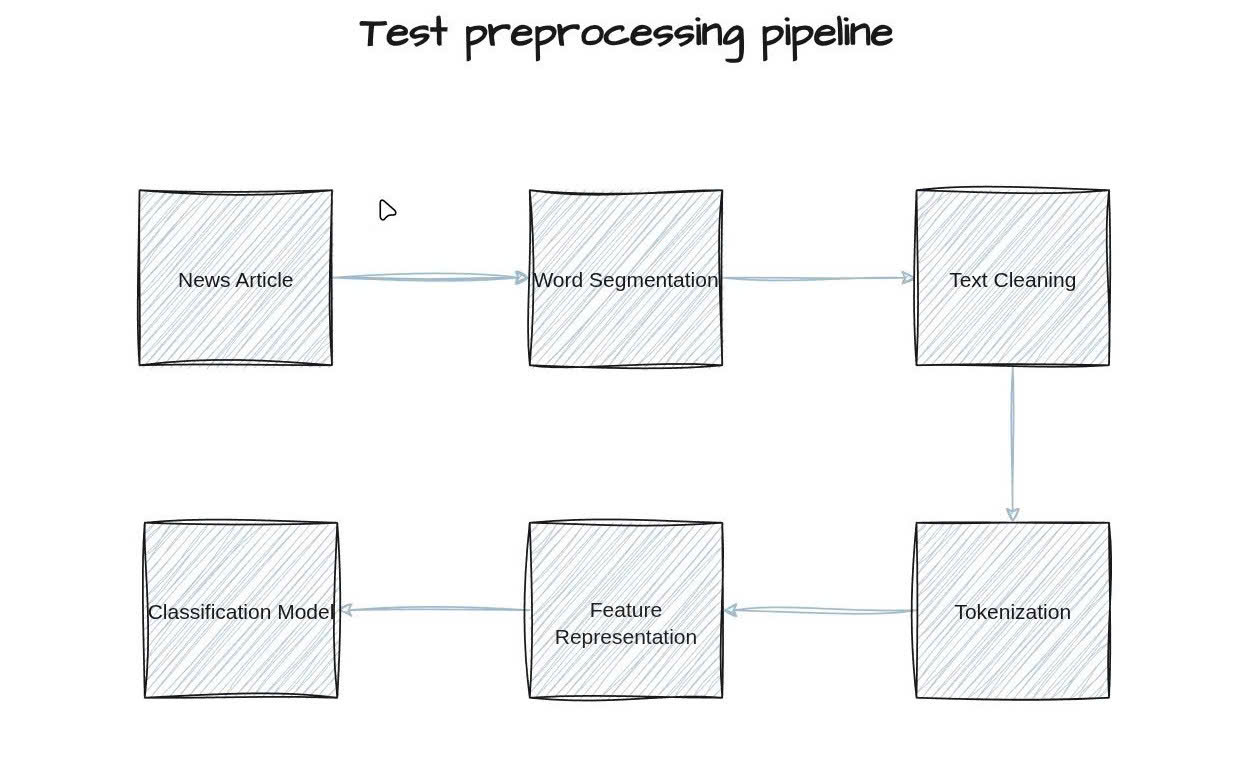
\includegraphics[width=0.95\textwidth]{textpreprocessing.jpg}
  \caption{Các bước tiền xử lý văn bản trước khi đưa vào mô hình học máy.}
  \label{fig:preprocessing}
\end{figure}

\subsection{Bài toán phân loại văn bản}
Phát hiện tin giả về bản chất là bài toán phân loại nhị phân trong đó mỗi văn bản được gán nhãn “thật” hoặc “giả”. Mô hình cần học một hàm ánh xạ từ không gian đặc trưng của văn bản sang tập nhãn, sao cho ranh giới quyết định phân tách tốt nhất hai lớp trên dữ liệu chưa quan sát.


\section{Xử lý ngôn ngữ tự nhiên tiếng Việt}

\subsection{Đặc điểm ngôn ngữ tiếng Việt}

Tiếng Việt là ngôn ngữ đơn lập, không biến hình, với các đặc điểm khác biệt so với tiếng Anh và nhiều ngôn ngữ châu Âu:

\begin{itemize}[leftmargin=2em]
  \item \textbf{Không có khoảng cách giữa các âm tiết:} Ranh giới từ và âm tiết trong tiếng Việt không trùng nhau. Ví dụ, ``thành phố'' là một từ nhưng được viết thành hai âm tiết riêng biệt.
  \item \textbf{Từ ghép và từ láy:} Nhiều khái niệm được biểu đạt bằng tổ hợp nhiều âm tiết, ví dụ từ ghép ``học\_sinh'', ``kinh\_tế'', hay từ láy ``lung\_linh''.
  \item \textbf{Thanh điệu:} Tiếng Việt có 6 thanh điệu, ảnh hưởng quan trọng đến ngữ nghĩa nhưng không ảnh hưởng đến cấu trúc hình thái học.
  \item \textbf{Ngôn ngữ cô lập:} Quan hệ ngữ pháp được biểu đạt qua trật tự từ và các hư từ, không qua biến đổi hình thái.
\end{itemize}

Những đặc điểm này của tiếng Việt đòi hỏi bước tiền xử lý đặc thù -- đặc biệt là \textit{phân đoạn từ} -- trước khi được dùng trong các mô hình học máy và học sâu.

\subsection{Phân đoạn từ (Word Segmentation)}

Phân đoạn từ là bước xác định ranh giới các từ trong câu. Đối với tiếng Việt hiện nay, các mô hình xử lý ngôn ngữ tự nhiên (Natural Language Processing -- NLP), đặc biệt là PhoBERT, được huấn luyện trên dữ liệu đã được phân đoạn.

\textbf{Ví dụ:}
\begin{quote}
\textit{Trước:} ``Thành phố Hồ Chí Minh là trung tâm kinh tế lớn nhất Việt Nam.''\\
\textit{Sau:} ``Thành\_phố Hồ\_Chí\_Minh là trung\_tâm kinh\_tế lớn nhất Việt\_Nam.''
\end{quote}

Trong nghiên cứu này, nhóm sử dụng \textbf{VnCoreNLP RDRSegmenter}~\cite{nguyen2018vncorenlp} thông qua thư viện \texttt{py\_vncorenlp}. Đây là bộ phân đoạn cùng với bộ tokenizer mà mô hình \phobert được tiền huấn luyện,do đó đảm bảo được sự nhất quán về từ vựng

\subsection{Biểu diễn văn bản số}

Để các mô hình có thể học được, dữ liệu cần phải được chuyển đổi sang dạng số. Nghiên cứu này sử dụng ba phương pháp:

\begin{enumerate}[leftmargin=2.5em]
  \item \textbf{TF-IDF:} Vectơ đặc trưng dựa trên tần suất từ, phương pháp này phù hợp cho LR và SVM.
  \item \textbf{Nhúng từ (Word Embedding):} Vectơ dày đặc học được~\cite{mikolov2013word2vec}, khởi tạo từ FastText tiếng Việt~\cite{bojanowski2017fasttext}, phù hợp cho BiLSTM.
  \item \textbf{Mã hóa cặp byte (Byte-Pair Encoding -- BPE):} Tách từ thành các đơn vị con, phương pháp này được dùng cho PhoBERT.
\end{enumerate}

\section{Học máy}

\subsection{Định nghĩa}

Với sự phát triển của khoa học công nghệ, các ứng dụng tự động ngày càng trởnên phổ biến hơn trong đời sống chúng ta, một phần là nhờ vào các thuật toán học máy. Học máy (Machine Learning – ML) là một nhánh của lĩnh vực trí tuệ nhân tạo (Artificial Intelligence – AI), chuyên nghiên cứu và phát minh các thuật toán cho phép máy tính có khả năng tự vận hành một công việc nhất định bằng các bộ dữ liệu đã có
mà không cần can thiệp nhiều từ lập trình viên.

Các thuật toán máy học thường được chia thành 2 loại chính, đó là:

Học có giám sát (Supervised Learning) gồm các thuật toán giúp máy tính xây dựng một hàm dựa trên dữ liệu có sẵn và đã được gán nhãn để có thể xác định nhãn của một dữ liệu mới.

Học không giám sát (Unsupervised Learning) gồm các thuật toán cho phép máy tính học từ các dữ liệu có sẵn nhưng chưa được gán nhãn. Từ đó, phân các dữ liệu này thành các cụm theo yêu cầu.

\subsection{Một số thuật toán học máy tiêu biểu}
\subsubsection{Hồi quy Logistic (Logistic Regression -- LR)}
Hồi quy Logistic (Logistic Regression)~\cite{cox1958regression} là một thuật toán học máy có giám sát được sử dụng phổ biến trong các bài toán phân lớp nhị phân. Thuật toán này mô hình hóa mối quan hệ giữa các đặc trưng đầu vào và xác suất thuộc về một lớp thông qua một hàm logistic (sigmoid). Cụ thể, dữ liệu huấn luyện được biểu diễn dưới dạng các vector đặc trưng trong không gian nhiều chiều. Thuật toán sẽ học các tham số của mô hình sao cho xác suất dự đoán phù hợp nhất với nhãn thực tế của dữ liệu huấn luyện.

Khi có một điểm dữ liệu mới (chưa có nhãn), mô hình sẽ tính toán giá trị tuyến tính của điểm đó dựa trên các trọng số đã học, sau đó đưa kết quả qua hàm sigmoid để thu được một giá trị xác suất trong khoảng từ 0 đến 1. Dựa trên một ngưỡng phân loại xác định trước (thường là 0.5), điểm dữ liệu mới sẽ được gán vào một trong hai lớp tương ứng. Nếu xác suất dự đoán lớn hơn hoặc bằng ngưỡng, điểm dữ liệu sẽ được gán vào lớp thứ nhất; ngược lại, nó sẽ được gán vào lớp còn lại. Nhờ cơ chế này, Logistic Regression cho phép thực hiện phân lớp một cách hiệu quả và dễ diễn giải trong nhiều bài toán thực tế.

\subsubsection{Máy vectơ hỗ trợ (Support Vector Machine -- SVM)}

Máy vectơ hỗ trợ (Support Vector Machine -- SVM)~\cite{cortes1995svm} là một thuật toán học máy có giám sát được sử dụng phổ biến trong các bài toán phân lớp nhị phân. Đối với bài toán phát hiện tin giả, SVM được sử dụng để phân loại văn bản thành hai lớp là “thật” và “giả”. Thuật toán hoạt động dựa trên việc tìm một siêu phẳng (hyperplane) trong không gian đặc trưng sao cho có thể phân tách hai lớp dữ liệu một cách tối ưu.

Cụ thể, các dữ liệu huấn luyện sau khi được biểu diễn dưới dạng vector đặc trưng (ví dụ như TF-IDF) sẽ được ánh xạ vào không gian nhiều chiều. Trong không gian này, SVM tìm một siêu phẳng sao cho khoảng cách từ siêu phẳng đến các điểm gần nhất của mỗi lớp là lớn nhất. Khoảng cách này được gọi là biên (margin). Những điểm dữ liệu nằm gần siêu phẳng nhất và quyết định vị trí của nó được gọi là các vector hỗ trợ (support vectors).

Khi đã xác định được siêu phẳng tối ưu, với một điểm dữ liệu mới, mô hình sẽ xác định vị trí của điểm đó so với siêu phẳng để gán nhãn tương ứng. Nếu điểm dữ liệu nằm về một phía của siêu phẳng, nó sẽ được gán vào lớp thứ nhất; nếu nằm về phía còn lại, nó sẽ được gán vào lớp thứ hai. Nhờ cơ chế tối đa hóa biên phân tách, SVM thường đạt hiệu quả cao trong các bài toán phân loại văn bản nhị phân như phát hiện tin giả.

\begin{figure}[H]
  \centering
  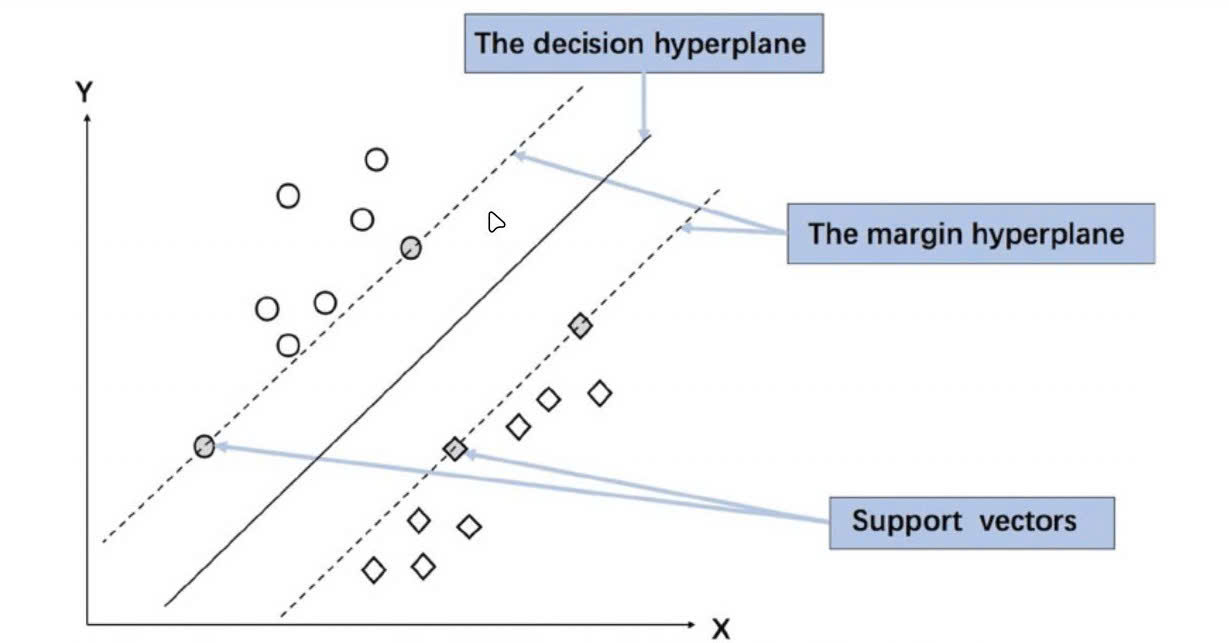
\includegraphics[width=0.95\textwidth]{svm.jpg}
  \caption{Minh họa thuật toán nhị phân SVM (phỏng theo \cite{cortes1995svm})}
  \label{fig:svm}
\end{figure}

\subsection{Biểu diễn đặc trưng cơ bản}
\subsubsection{Tần suất từ -- Tần suất tài liệu nghịch đảo (TF-IDF)}
TF-IDF (Term Frequency - Inverse Document Frequency)~\cite{sparkjones1972idf} là một trong những cách biểu diễn văn bản phổ biến trong các bài toán xử lý ngôn ngữ tự nhiên và phân loại văn bản. Phương pháp này đánh giá tính quan trọng của một từ trong một tài liệu nào đó theo tần suất xuất hiện của từ đó trong tài liệu và tính phổ biến của từ đó trong toàn bộ tập dữ liệu.

Term Frequency (TF) mô tả tần suất xuất hiện của một từ $t$ trong một tài liệu $d$. Để giảm thiên lệch do chiều dài tài liệu, TF thường được normal hóa theo tổng từ trong tài liệu:

\[
TF(t, d) = \frac{f_{t,d}}{\sum_{t' \in d} f_{t',d}}
\]

Trong đó, $f_{t,d}$ là số lần lặp lại của từ $t$ trong văn bản $d$.

Inverse Document Frequency (IDF) được sử dụng để giảm trọng số của từ có tần suất lặp lại nhiều trong nhiều văn bản và tăng trọng số của từ có tính phân biệt cao. Cụ thể, công thức tính IDF như sau:

\[
IDF(t) = \log \left( \frac{N}{df_t} \right)
\]

trong đó $N$ là tổng số tài liệu trong tập dữ liệu và $df_t$ là số tài liệu chứa từ $t$.

Giá trị TF-IDF của một từ $t$ trong tài liệu $d$ được xác định bằng tích của hai thành phần trên:

\[
TF\text{-}IDF(t, d) = TF(t, d) \times IDF(t)
\]

Kết quả đạt được là một trọng số thực đại diện cho độ quan trọng tương đối của từng từ trong tài liệu đó. Sau khi tính toán cho toàn bộ từ vựng, mỗi tài liệu sẽ được biểu diễn dưới hình thức một vector đặc trưng với độ dài bằng tổng số từ trong từ điển. Các vector này thường là thưa (sparse) và thường dùng như một đầu vào cho các mô hình học máy truyền thống như Hồi quy Logistic (Logistic Regression) và Máy vectơ hỗ trợ (Support Vector Machine) cho các ứng dụng phân loại văn bản, như phát hiện thông tin giả.

\section{Học sâu}

\subsection{Định nghĩa}
Học sâu (Deep Learning) là một phương pháp trong học máy sử dụng các mô hình mạng nơ-ron nhân tạo có nhiều lớp nơ-ron ẩn nhằm giúp các hệ thống có khả năng học các đặc trưng phức tạp từ dữ liệu đầu vào. So với các phương pháp học máy truyền thống, trong đó các đặc trưng được tạo ra một cách thủ công, học sâu có khả năng tự động trích xuất các đặc trưng từ dữ liệu thông qua quá trình huấn luyện trên dữ liệu lớn.

Mỗi mô hình học sâu được xây dựng bằng các lớp nơ-ron được kết nối với nhau theo từng tầng. Dữ liệu đầu vào được truyền thông qua các lớp nơ-ron này theo cơ chế lan truyền tiến (feedforward), trong đó dữ liệu được xử lý tại từng lớp bằng các phép biến đổi tuyến tính kết hợp với hàm kích hoạt phi tuyến nhằm đạt được biểu diễn tại mức trừu tượng cao. Trong quá trình huấn luyện, các tham số của mô hình được điều chỉnh thông qua thuật toán lan truyền ngược (backpropagation) ~\cite{rumelhart1986backprop} nhằm đạt được hàm mất mát tối thiểu.

Bên cạnh đó, nhờ có tính học nhiều tầng và khả năng học biểu diễn tự động, học sâu đã đạt được hiệu quả cao trong nhiều lĩnh vực như thị giác máy tính, xử lý ngôn ngữ tự nhiên, nhận dạng tiếng nói,... Đối với bài toán phát hiện tin giả, các mô hình học sâu như BiLSTM và PhoBERT có khả năng khai thác thông tin ngữ cảnh và mối quan hệ giữa các từ một cách hiệu quả hơn so với các phương pháp truyền thống.

\subsection{Mạng nơ-ron nhân tạo (Artificial Neural Network)}
Dựa trên cơ chế hoạt động của neuron trong cơ thể, các nhà khoa học đã xây dựng mô hình mạng nơ-ron nhân tạo nhằm mô phỏng hoạt động xử lý thông tin của bộ não người. Trong cơ thể, neuron là đơn vị cấu trúc cơ bản của hệ thần kinh. Mô hình neuron cơ bản gồm thân tế bào, sợi nhánh, và sợi trục. Thân tế bào neuron là nơi chứa nhân tế bào, sợi nhánh là nơi neuron nhận tín hiệu, và sợi trục là nơi neuron gửi tín hiệu cho neuron khác. Khi neuron nhận tín hiệu thông qua sợi nhánh, neuron sẽ thực hiện hoạt động xử lý và tổng hợp tín hiệu. Nếu tín hiệu sau khi xử lý lớn hơn ngưỡng nào đó, neuron sẽ gửi tín hiệu cho neuron khác thông qua sợi trục. Mô hình hoạt động của neuron đã được mô hình hóa trong mạng nơ-ron nhân tạo thông qua một hàm tính, trong đó nhiều tín hiệu đầu vào sẽ tạo nên tín hiệu đầu ra duy nhất. Vai trò của ngưỡng kích hoạt được mô phỏng thông qua hàm kích hoạt (Activation Function), quyết định xem neuron có phát tín hiệu hay không.

Mạng nơ-ron nhân tạo là một tập hợp các neuron nhân tạo được tổ chức thành nhiều lớp, bao gồm lớp đầu vào, một hoặc nhiều lớp ẩn và lớp đầu ra. Mỗi lớp ẩn có thể bao gồm một hoặc nhiều neuron nhân tạo. Các neuron trong một lớp được kết nối với các neuron ở lớp kế tiếp thông qua các trọng số, và không tồn tại kết nối giữa các neuron trong cùng một lớp.

Trong quá trình huấn luyện, mạng nơ-ron nhân tạo thực hiện cơ chế lan truyền tiến (Feedforward), trong đó dữ liệu đầu vào được truyền qua từng lớp và được biến đổi thông qua các trọng số tương ứng để tạo ra kết quả dự đoán ở đầu ra. Để đánh giá độ chính xác của dự đoán, một hàm mất mát (Loss Function) được sử dụng nhằm tính toán sai số giữa giá trị dự đoán và nhãn thực tế. Dựa trên sai số này, các tham số của mô hình sẽ được cập nhật thông qua thuật toán lan truyền ngược (Backpropagation) nhằm giảm thiểu sai số. Quá trình này được lặp lại nhiều lần cho đến khi mô hình đạt được trạng thái hội tụ.

Trong các kiến trúc mạng nơ-ron hiện đại, nhiều mô hình đã được phát triển nhằm xử lý các loại dữ liệu khác nhau. Đối với bài toán xử lý văn bản, các kiến trúc mạng nơ-ron hồi quy (Recurrent Neural Network -- RNN) và các mô hình dựa trên Transformer được sử dụng phổ biến.

\subsubsection{Một số thành phần cần chú ý}

Hàm kích hoạt (Activation Function) là một trong những thành phần quan trọng trong mô hình mạng nơ-ron nhân tạo, có ý nghĩa quyết định đến việc liệu một tín hiệu đã được tổng hợp tại một nơ-ron có được truyền đi đến nơ-ron trong lớp kế tiếp hay không. Sau khi thực hiện quá trình tính toán các giá trị đầu vào được nhân với các trọng số tương ứng rồi cộng lại tại từng nơ-ron trong mạng nơ-ron nhân tạo, ta sử dụng hàm kích hoạt để tạo tính phi tuyến trong mô hình mạng nơ-ron. Bởi vậy mà mô hình mạng nơ-ron có khả năng học được các mối quan hệ trong dữ liệu phức tạp. Một số hàm kích hoạt được sử dụng trong mạng nơ-ron nhân tạo là Sigmoid, Tanh, ReLU. Đối với các bài toán về phân loại dữ liệu, đặc biệt là bài toán phân loại nhị phân, hàm Sigmoid được sử dụng trong lớp output để dự đoán ra kết quả xác suất trong một khoảng giá trị từ 0 đến 1, trong khi hàm Softmax được sử dụng khi cần phân phối xác suất trên nhiều lớp.

Để xác định được độ chính xác của mô hình trong quá trình huấn luyện, người ta sử dụng hàm mất mát (Loss Function) với mục đích đo lường sai số giữa dự đoán và nhãn. Trong bài toán phân loại văn bản, hàm mất mát thường được sử dụng là hàm Cross-Entropy do có khả năng đo được sự chênh lệch giữa phân phối xác suất dự đoán và phân phối xác suất thực tế. Giá trị của hàm mất mát càng nhỏ thì mô hình càng đưa ra dự đoán gần với nhãn đúng.

Quá trình huấn luyện mạng nơ-ron nhân tạo diễn ra qua hai quá trình chính: lan truyền tiến và lan truyền ngược. Trong quá trình lan truyền tiến, dữ liệu đầu vào được truyền qua từng lớp của mạng nơ-ron nhân tạo. Trong quá trình truyền dữ liệu qua từng lớp của mạng nơ-ron nhân tạo, các phép biến đổi tuyến tính và phi tuyến được thực hiện. Sau khi tính được kết quả của hàm mất mát, thuật toán lan truyền ngược được thực hiện với mục đích tính đạo hàm của sai số với từng tham số của mạng nơ-ron nhân tạo. Các tham số của mạng nơ-ron nhân tạo được cập nhật với thuật toán tối ưu hóa phổ biến nhất là thuật toán Gradient Descent với mục đích giảm thiểu sai số.

Trong quá trình huấn luyện các mạng nhiều tầng, có thể xuất hiện các hiện tượng như mất mát hoặc bùng nổ gradient khi giá trị đạo hàm trở nên quá nhỏ hoặc quá lớn. Những vấn đề này ảnh hưởng đến tốc độ và độ ổn định của quá trình học. Các kiến trúc hiện đại như LSTM và Transformer được thiết kế nhằm hạn chế những hạn chế này, giúp mô hình học được các quan hệ dài hạn trong dữ liệu chuỗi, đặc biệt hiệu quả trong các bài toán xử lý ngôn ngữ tự nhiên như phát hiện tin giả.

\subsection{Mạng nơ-ron hồi quy (Recurrent Neural Network -- RNN)}

RNN là một mô hình học sâu được xây dựng nhằm xử lý dữ liệu tuần tự thông qua việc giữ lại thông tin từ các trạng thái trước đó ~\cite{elman1990rnn}. Nhờ đó, RNN có khả năng nhớ và sử dụng các mối liên hệ giữa các phần tử trong dữ liệu tuần tự để tạo ra các kết quả có ngữ cảnh và ý nghĩa hơn. 

Dữ liệu tuần tự có thể là văn bản, dữ liệu thời gian, hoặc các tín hiệu âm thanh trong đó các phần tử có sự liên kết với nhau dựa trên các ngữ nghĩa hoặc các quy luật xác định. So với các mạng nơ-ron truyền thống được sử dụng để xử lý các dữ liệu đầu vào độc lập với nhau, RNN được trang bị một vòng lặp nội tại để truyền thông tin trong từng bước thời gian.

Tuy nhiên, mặc dù có khả năng ghi nhớ thông tin thông qua các bước thời gian, RNN truyền thống vẫn tồn tại một số hạn chế. Khi chuỗi dữ liệu được trình bày theo một chuỗi có kích thước lớn, quá trình lan truyền ngược sai số qua nhiều bước thời gian có thể làm cho gradient trở nên cực kỳ nhỏ hoặc cực kỳ lớn. Lúc này gradient có xu hướng bị mất đi (vanishing gradient) hoặc bùng nổ gradient (exploding gradient)~\cite{bengio1994vanishing,pascanu2013gradient}. Khi gradient bị suy giảm quá mức, mô hình sẽ gặp khó khăn trong việc học và ghi nhớ các phụ thuộc dài hạn giữa các phần tử trong chuỗi. Điều này ảnh hưởng trực tiếp đến hiệu quả của RNN trong các bài toán xử lý văn bản, nơi mà ngữ nghĩa của một từ có thể phụ thuộc vào các từ xuất hiện ở vị trí xa trong câu hoặc đoạn văn. Để khắc phục những hạn chế này, các kiến trúc cải tiến như Bộ nhớ dài-ngắn hạn (Long Short-Term Memory -- LSTM) đã được đề xuất nhằm tăng cường khả năng ghi nhớ thông tin dài hạn và cải thiện hiệu suất của mô hình trên dữ liệu tuần tự.

\subsection{Bộ nhớ dài-ngắn hạn (Long Short-Term Memory -- LSTM)}
Bộ nhớ dài-ngắn hạn (Long Short-Term Memory - LSTM) ~\cite{hochreiter1997lstm} là một kiến trúc RNN được thiết kế để giải quyết một số hạn chế của RNN trong khả năng ghi nhớ thông tin dài hạn. Trong khi kiến trúc RNN đơn giản sử dụng một trạng thái ẩn đơn giản để truyền thông tin từ một bước thời gian sang một bước thời gian khác, kiến trúc LSTM được trang bị một bộ nhớ tế bào (memory cell) và ba cơ chế cổng kiểm soát, gồm cổng quên, cổng đầu vào, và cổng đầu ra.

\begin{figure}[H]
  \centering
  \includegraphics[width=0.95\textwidth]{LSTM.jpeg}
  \caption{Minh họa cấu trúc mạng LSTM~\cite{jm3}.}
  \label{fig:LSTM}
\end{figure}

Một đặc điểm nổi bật của mạng LSTM là khả năng học và nhớ phụ thuộc lâu dài (long-term dependencies) trong dữ liệu tuần tự. Điều này đặc biệt quan trọng trong những tình huống yêu cầu sự hiểu biết ngữ cảnh lâu dài, chẳng hạn như xử lý ngôn ngữ tự nhiên (NLP), dịch thuật máy, nhận dạng giọng nói, hoặc dự đoán thời gian.

Một cách đặc biệt, bằng việc giải quyết vấn đề gradient biến mất - một vấn đề lớn trong việc huấn luyện mạng lưới hồi tiếp sâu, mạng lưới hồi tiếp lâu dài không chỉ đảm bảo sự ổn định của quá trình học tập, mà đặc biệt phù hợp với những bài toán xử lý văn bản như phân loại tin tức.

Trong cấu trúc của LSTM, mỗi cell được quản lý bởi các cổng chính là: cổng quên (forget gate), cổng vào (input gate), và cổng ra (output gate). Cổng quên được định nghĩa là xác định những thông tin nào cần phải nhớ hay không. Cổng này đóng vai trò quan trọng trong việc loại bỏ những thông tin không cần thiết nữa trong bộ nhớ của LSTM. Từ đó, các thông tin không cần thiết không gây ra nhiễu trong quá trình học nhớ lâu dài. Kế tiếp đó là cổng vào xác định những thông tin nào cần phải học trong bộ nhớ hiện tại. Kết hợp giữa cổng quên và cổng vào là cách mà LSTM học nhớ lâu dài một cách chọn lọc. Cuối cùng là cổng ra xác định những thông tin nào cần phải sử dụng trong bộ nhớ để tạo ra trạng thái ẩn trong thời điểm hiện tại. Từ đó, nó ảnh hưởng đến đầu ra của mô hình. Thông qua các cổng trong cấu trúc của LSTM, nó đã học nhớ lâu dài các phụ thuộc trong chuỗi dữ liệu một cách hiệu quả so với RNN truyền thống.

Tuy nhiên, mạng LSTM thông thường chỉ khai thác thông tin trong một chiều, tức là từ quá khứ đến hiện tại. Đối với các bài toán xử lý ngôn ngữ tự nhiên, ngữ nghĩa của một từ không chỉ phụ thuộc vào các từ đứng trước mà có thể phụ thuộc cả về các từ đứng sau trong câu. Vì vậy, kiến trúc mạng LSTM hai chiều (Bidirectional LSTM - BiLSTM) được đề xuất để mở rộng khả năng biểu diễn của mạng LSTM trong các bài toán phân loại văn bản, như bài toán phát hiện tin giả.


\subsection{Mạng LSTM hai chiều (Bidirectional LSTM)}

Kiến trúc mạng LSTM hai chiều, còn được gọi là Bidirectional LSTM – BiLSTM, là một dạng mở rộng của mạng LSTM. Trong khi LSTM truyền thống chỉ xử lý chuỗi theo một chiều thời gian, thường là từ trái sang phải (từ quá khứ đến hiện tại), thì BiLSTM bao gồm hai mạng LSTM hoạt động song song. Một mạng xử lý chuỗi theo chiều thuận (forward), tức là từ phần tử đầu tiên đến phần tử cuối cùng; mạng còn lại xử lý chuỗi theo chiều ngược (backward), tức là từ cuối về đầu. Cụ thể, với mỗi thời điểm, mạng LSTM thuận sử dụng các phần tử xuất hiện trước đó trong chuỗi dữ liệu để tạo ra một trạng thái ẩn. Ngược lại, mạng LSTM ngược sử dụng các phần tử xuất hiện sau đó để tạo ra một trạng thái ẩn. Hai trạng thái ẩn này sau đó được kết hợp lại để tạo ra một trạng thái cuối cùng để tạo thành biểu diễn ngữ cảnh đầy đủ hơn cho từng phần tử trong chuỗi.

Trong các bài toán xử lý ngôn ngữ tự nhiên, không chỉ có nghĩa của một từ được quyết định bởi từ ngữ trước đó mà còn được quyết định một phần bởi từ ngữ sau đó. Vì vậy, BiLSTM cho phép mô hình nắm bắt được ngữ cảnh của một từ một cách toàn diện hơn so với phương pháp đơn giản của LSTM một chiều. Trong bài toán phát hiện tin giả, việc khai thác ngữ cảnh của một câu và một đoạn văn được cho là có lợi cho mô hình hiểu được nội dung và sắc thái của thông tin, từ đó nâng cao được khả năng phân loại được “thật” và “giả”.

\begin{figure}[H]
  \centering
  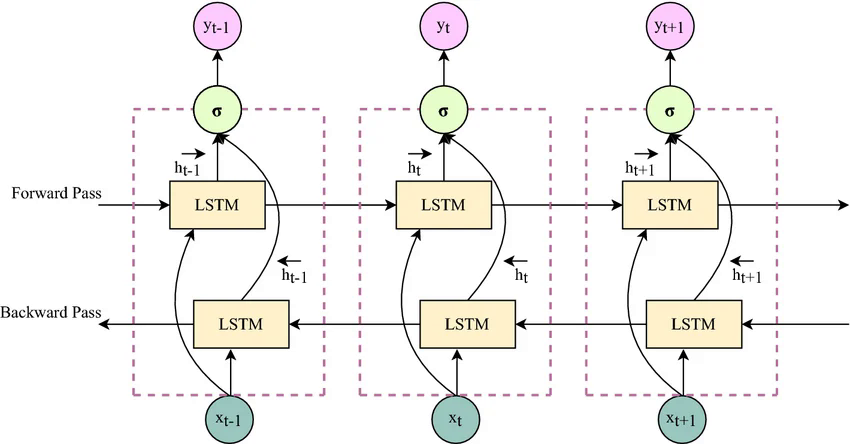
\includegraphics[width=0.95\textwidth]{bilstm.png}
  \caption{Minh họa cấu trúc mạng LSTM hai chiều~\cite{article}.}
  \label{fig:BiLSTM}
\end{figure}


\subsection{Cơ chế chú ý (Attention Mechanism)}


Cơ chế chú ý (Attention Mechanism) ~\cite{bahdanau2015attention} được đưa ra để cải thiện các nhược điểm của các mô hình xử lý chuỗi khi phải nén toàn bộ thông tin của một câu thành một vector. Thay vì mỗi phần tử trong chuỗi đều được tính là có độ quan trọng ngang nhau, cơ chế chú ý cho phép các mô hình tự động học được trọng số cho từng bước trong chuỗi, để tập trung nhiều hơn vào các phần tử quan trọng đối với các tác vụ dự đoán.

Giả sử $\{h_1, h_2, \dots, h_T\}$ là các trạng thái ẩn thu được từ mô hình LSTM hoặc BiLSTM. 
Tại mỗi bước thời gian $t$, một điểm số $e_t$ được tính để đo mức độ liên quan của trạng thái ẩn $h_t$ đối với đầu ra cuối cùng:
\begin{align}
  e_t &= \mathbf{v}^{\top} \tanh(\mathbf{W}_a \overleftrightarrow{\mathbf{h}}_t)
\end{align}

Các điểm số này sau đó được chuẩn hóa thông qua hàm softmax để tạo thành trọng số chú ý $\alpha_t$:
\begin{align}
  \alpha_t &= \frac{\exp(e_t)}{\sum_{k=1}^{T} \exp(e_k)}
\end{align}

Cuối cùng, vector ngữ cảnh $c$ được tính bằng tổng có trọng số của các trạng thái ẩn:
\begin{align}
  \mathbf{c} &= \sum_{t=1}^{T} \alpha_t \overleftrightarrow{\mathbf{h}}_t
\end{align}

Trong đó, $\alpha_t$ thể hiện mức độ mà từng từ hoặc từng bước trong thời gian đã đóng góp vào biểu diễn cuối cùng của câu. Từ quan trọng sẽ có trọng số cao hơn, còn từ không quan trọng có trọng số nhỏ hơn. Bằng cách này, mô hình có khả năng tập trung vào các thành phần quan trọng của văn bản, chứ không xử lý toàn bộ văn bản một cách đồng đều.

Trong trường hợp của bài toán phát hiện tin giả, cơ chế chú ý cho phép mô hình phát hiện ra từ hoặc cụm từ quan trọng có tác động lớn đến nội dung và ý nghĩa của thông tin, ví dụ, từ thể hiện quan điểm cực đoan, từ thể hiện thông tin gây hiểu lầm, từ thể hiện chi tiết bất thường. Điều này có thể giúp nâng cao khả năng phân biệt được giữa tin ``thật'' và ``giả''.

Đáng chú ý, cơ chế tự chú ý (self-attention) là nền tảng cốt lõi của kiến trúc Transformer. Thay vì chỉ tính trọng số dựa trên một trạng thái ẩn duy nhất, self-attention cho phép mỗi phần tử trong chuỗi tương tác trực tiếp với tất cả các phần tử khác, từ đó xây dựng biểu diễn ngữ cảnh toàn cục hiệu quả hơn. Đây chính là cơ sở cho các mô hình ngôn ngữ hiện đại như BERT và PhoBERT được trình bày ở phần tiếp theo.

\subsection{Mô hình Transformer và PhoBERT}

Transformer là một kiến trúc học sâu dựa trên cơ chế tự chú ý (self-attention)~\cite{vaswani2017attention}, được đề xuất nhằm giải quyết các hạn chế của các mô hình tuần tự như RNN và LSTM khi áp dụng trong xử lý phụ thuộc dài hạn. So với các mô hình xử lý dữ liệu theo từng bước thời gian,Transformer cho phép xử lý toàn bộ chuỗi dữ liệu đầu vào một cách đồng thời, từ đó tăng khả năng song song hóa và hiệu quả huấn luyện.

Kiến trúc ban đầu củaTransformer bao gồm các thành phần chính là encoder và decoder. Tuy nhiên, trong các mô hình ngôn ngữ tiền huấn luyện như BERT~\cite{devlin2019bert} và PhoBERT~\cite{phobert2020}, chỉ sử dụng phần encoder củaTransformer để xây dựng biểu diễn ngữ cảnh cho văn bản. Vì vậy, trong phạm vi đề tài nghiên cứu này, chúng tôi tập trung vào kiến trúc của Transformer encoder.

\begin{figure}[H]
  \centering
  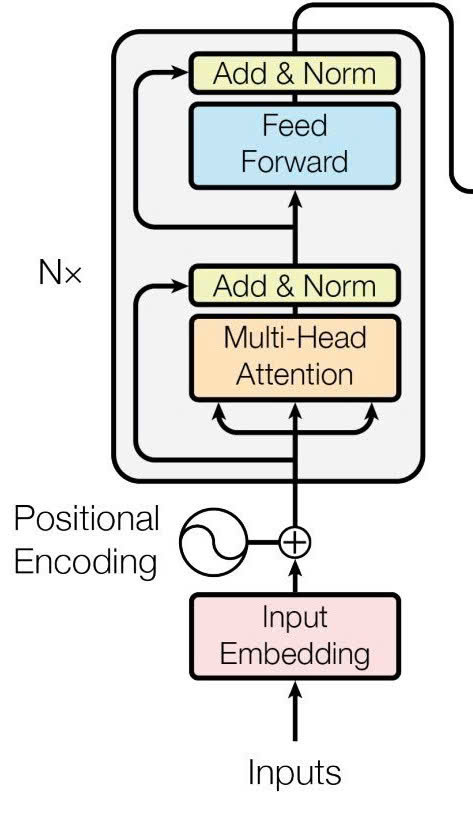
\includegraphics[width=0.5\textwidth]{encoder.jpg}
  \caption{Minh họa khối encoder của Transformer \cite{vaswani2017attention}.}
  \label{fig:encoder}
\end{figure}

Trong hình trên, có thể thấy được cấu trúc của một khối trong Transformer. Đầu vào của mô hình bao gồm các vector embedding của các từ trong câu và thông tin vị trí. Thông tin vị trí được thêm để đảm bảo thứ tự của các từ trong một câu. Cơ chế attention không xử lý các thông tin một cách tuần tự, vì vậy thông tin vị trí được thêm để đảm bảo thứ tự của các từ trong một câu.

Một khối trong mô hình Transformer được tạo thành từ hai phần. Phần đầu tiên là cơ chế attention multi-head, cho phép các từ trong một câu tương tác trực tiếp với các từ trong cùng một câu để tính toán độ liên quan. Bằng cơ chế attention, các quan hệ ngữ nghĩa trong một văn bản được tính toán mà không bị phụ thuộc vào khoảng cách vị trí. Kết quả của cơ chế attention được đưa đến một bước tính toán (Add \& Norm) nhằm ổn định quá trình huấn luyện.

Thành phần thứ hai là mạng truyền thẳng từng vị trí (Positionwise Feed-Forward Network - FFN), thực hiện các phép biến đổi phi tuyến trên từng vector đầu ra của lớp attention. Sau đó, một phép  Add \& Norm thứ hai được áp dụng. Các khối encoder được xếp chồng nhiều lần để tăng khả năng biểu diễn của mô hình.

Dựa trên khả năng học biểu diễn ngữ cảnh toàn cục thông qua self-attention và khả năng xử lý song song hiệu quả, Transformer đã trở thành nền tảng của các mô hình ngôn ngữ hiện đại. PhoBERT ~\cite{phobert2020} được xây dựng dựa trên kiến trúc của RoBERTa ~\cite{liu2019roberta}, một Transformer encoder nhiều tầng được tiền huấn luyện trên lượng lớn dữ liệu văn bản tiếng Việt.

Trong bài toán phát hiện tin giả, vector tương ứng với token đặc biệt \texttt{[CLS]} được tận dụng như một biểu diễn tổng quan của văn bản và được đi qua một lớp phân loại để dự đoán các nhãn ``thật'' hay ``giả''. Sử dụng biểu diễn ngữ cảnh sâu từ PhoBERT giúp mô hình hiểu rõ hơn nội dung cũng như sắc thái của văn bản, từ đó cải thiện khả năng phân loại.

\section{Kết luận chương}

Chương này đã trình bày nền tảng lý thuyết cho bốn mô hình so sánh trong nghiên cứu. Từ LR tuyến tính đến SVM phi tuyến, từ BiLSTM tuần tự đến Transformer song song, mỗi mô hình phản ánh một giai đoạn phát triển của NLP. Chương tiếp theo mô tả bộ dữ liệu và quy trình tiền xử lý.

\clearpage

% ============================================================
%  CHƯƠNG 2 -- BỘ DỮ LIỆU VÀ TIỀN XỬ LÝ
% ============================================================

\chapter{Bộ dữ liệu và tiền xử lý}

\section{Thu thập và mô tả bộ dữ liệu}

\subsection{Nguồn dữ liệu}

Bộ dữ liệu bao gồm các bài viết tiếng Việt được thu thập từ hai nguồn chính: các bài đăng công khai trên Facebook và một số bài báo cũ trong thời gian diễn ra COVID-19. Mỗi bản ghi chứa tối thiểu hai trường chính:

\begin{itemize}[leftmargin=2em]
  \item \texttt{text}: nội dung văn bản của bài viết.
  \item \texttt{label}: nhãn phân loại (0 = Thật, 1 = Giả).
\end{itemize}

Sau khi thực hiện bước phân đoạn từ (\textit{word segmentation}), dữ liệu được lưu lại và được sử dụng làm đầu vào cho quá trình làm sạch và chia tập.

Tổng số bản ghi ban đầu của bộ dữ liệu là \textbf{\nRaw{} mẫu}.

\subsection{Phân phối nhãn}

\begin{figure}[H]
  \centering
  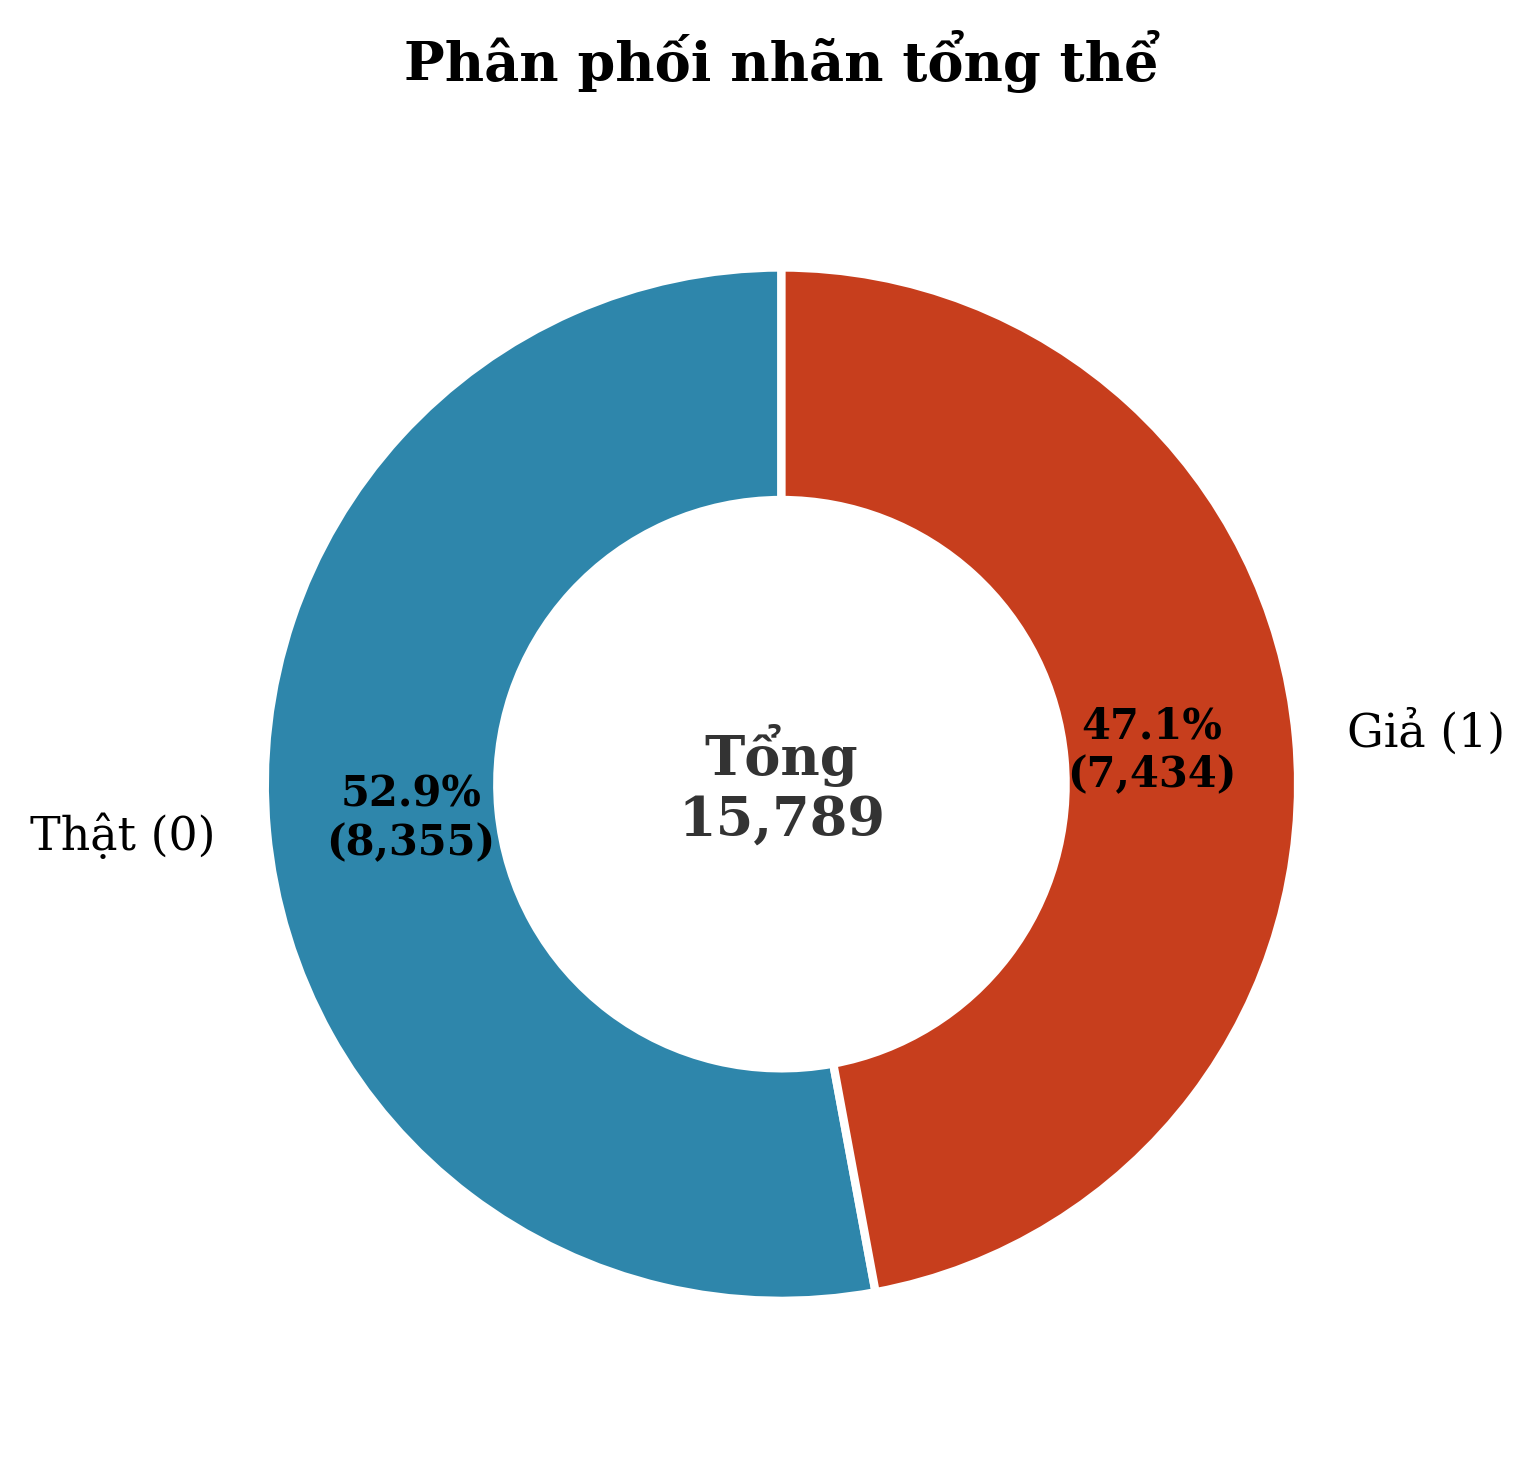
\includegraphics[width=0.5\textwidth]{fig0a_overall_distribution}
  \caption{Phân phối nhãn theo từng tập dữ liệu và tổng quan toàn bộ \nRaw{} mẫu}
  \label{fig:label_dist}
\end{figure}

\clearpage

Hình~\ref{fig:label_dist} minh họa phân phối nhãn tổng thể của toàn bộ tập dữ liệu. Có thể thấy, tỷ lệ tin thật và tin giả khá cân bằng, giúp đảm bảo mô hình không bị thiên lệch về một phía trong quá trình huấn luyện và đánh giá. Sự cân bằng này là yếu tố quan trọng để kết quả thực nghiệm phản ánh đúng hiệu quả của các phương pháp phân loại, đặc biệt trong bối cảnh dữ liệu thực tế thường có sự chênh lệch giữa các lớp.

\section{Tiền xử lý văn bản}

\subsection{Làm sạch và lọc dữ liệu}

Trước khi thực hiện bước chia tập huấn luyện, dữ liệu được tiến hành làm sạch 
nhằm loại bỏ nhiễu và hạn chế nguy cơ rò rỉ thông tin. Quy trình làm sạch bao gồm các bước sau:

\begin{enumerate}[leftmargin=2.5em]
  \item \textbf{Loại bỏ văn bản trùng lặp:} 
  Các bản ghi có nội dung \texttt{text} giống hệt nhau được loại bỏ, 
  chỉ giữ lại lần xuất hiện đầu tiên.

  \item \textbf{Loại bỏ văn bản rỗng hoặc giá trị thiếu:} 
  Các bản ghi có trường \texttt{text} bị thiếu (NaN) hoặc chuỗi rỗng 
  sau khi loại bỏ khoảng trắng được loại khỏi tập dữ liệu.

  \item \textbf{Loại bỏ văn bản quá ngắn:} 
  Những văn bản có ít hơn 10 từ bị loại bỏ do không cung cấp đủ 
  thông tin ngữ nghĩa cho bài toán phân loại. 
  Ngưỡng này được cấu hình thông qua tham số \texttt{min\_word\_count = 10}.

  \item \textbf{Đặt lại chỉ mục (index reset):} 
  Sau khi hoàn tất các bước trên, dữ liệu được đánh lại chỉ mục 
  nhằm đảm bảo tính nhất quán và thuận tiện cho quá trình xử lý tiếp theo.
\end{enumerate}

Sau quá trình làm sạch:

\begin{itemize}[leftmargin=2em]
  \item Số mẫu ban đầu: \nRaw
  \item Số mẫu bị loại bỏ: \nRemoved
  \item Số mẫu còn lại: \nClean
\end{itemize}

Quy trình làm sạch này giúp giảm nhiễu dữ liệu và đảm bảo rằng 
quá trình huấn luyện cũng như đánh giá mô hình không bị ảnh hưởng 
bởi các bản ghi trùng lặp hoặc không hợp lệ.

\subsection{Phân đoạn từ bằng VnCoreNLP}

Ngôn ngữ tiếng Việt được định nghĩa là một ngôn ngữ đơn lập, trong đó mỗi âm tiết được tách ra với khoảng trắng, mặc dù ranh giới từ không đồng nghĩa với ranh giới âm tiết. Ví dụ, cụm từ ``Việt Nam'' được định nghĩa là một đơn vị từ gồm hai âm tiết riêng biệt. Điều này tạo ra một thách thức quan trọng đối với xử lý ngôn ngữ tự nhiên vì định nghĩa của mỗi âm tiết là một từ đơn độc lập có thể gây ra sai lệch trong cấu trúc ngữ nghĩa của văn bản. Phân đoạn từ là một tiền xử lý quan trọng để đạt được chính xác trong biểu diễn và trích xuất đặc trưng.

Trong nghiên cứu này, quá trình phân đoạn từ được thư viện \texttt{py\_vncorenlp} thực hiện, dựa trên một bộ tách từ RDRSegmenter của VnCoreNLP~\cite{nguyen2018vncorenlp}. Quá trình này cũng được sử dụng trong phần tiền huấn luyện của mô hình PhoBERT. Sử dụng một bộ phân đoạn giống nhau trong việc xử lý dữ liệu đầu vào và từ vựng của mô hình ngôn ngữ trong phần tiền huấn luyện có khả năng tối đa hóa sự thống nhất, từ đó giảm thiểu độ sai lệch trong không gian biểu diễn và khả năng tổng quát hóa của mô hình.

Quy trình phân đoạn được triển khai theo các bước sau:

\begin{itemize}[leftmargin=2em]
  \item Tự động tải và lưu trữ mô hình VnCoreNLP tại thư mục cục bộ (\texttt{.vncorenlp}) nếu chưa tồn tại.
  \item Thực hiện phân đoạn đối với cả hai trường \texttt{title} và \texttt{text}.
  \item Chuẩn hóa văn bản trước khi phân đoạn, bao gồm:
  \begin{itemize}
    \item Loại bỏ dấu gạch dưới phát sinh từ các lần phân đoạn trước (nếu có).
    \item Chuẩn hóa khoảng trắng nhằm đảm bảo tính đồng nhất định dạng.
  \end{itemize}
\end{itemize}

Sau khi hoàn tất quá trình phân đoạn, các từ đa âm tiết được nối với nhau bằng dấu gạch dưới. Ví dụ:

\begin{quote}
\textit{Trước:} ``Chính phủ Việt Nam công bố chính sách mới'' \\
\textit{Sau:} ``Chính\_phủ Việt\_Nam công\_bố chính\_sách mới''
\end{quote}

Bước phân đoạn từ đóng vai trò then chốt trong việc cải thiện chất lượng biểu diễn đầu vào, đặc biệt đối với các mô hình dựa trên cơ chế \textit{subword tokenization} như PhoBERT. Nhờ đảm bảo sự tương thích giữa dữ liệu đã xử lý và từ điển tiền huấn luyện, quá trình này góp phần nâng cao độ ổn định và hiệu quả của mô hình trong giai đoạn huấn luyện và suy diễn.

\section{Chia tập dữ liệu}

\subsection{Chia phân tầng}
\label{sec:data_split}

Sau khi thực hiện phân đoạn từ, dữ liệu được chia thành ba tập: 
huấn luyện (train), kiểm định (validation) và kiểm tra (test). 
Quy trình này bao gồm bước làm sạch dữ liệu trước khi chia tập.

Việc chia tập được thực hiện theo chiến lược phân tầng 
(\textit{stratified split}) nhằm duy trì phân phối nhãn đồng đều 
trong cả ba tập. Cấu hình chia tập như sau:

\begin{itemize}[leftmargin=2em]
  \item Train: 70\%
  \item Validation: 15\%
  \item Test: 15\%
  \item \texttt{random\_state = 42}
\end{itemize}

Quy trình chia được thực hiện theo hai bước. 
Đầu tiên, 15\% dữ liệu được tách ra làm tập kiểm tra (test set). 
Sau đó, từ 85\% dữ liệu còn lại, tiếp tục tách một phần tương ứng 
15\% tổng dữ liệu ban đầu (xấp xỉ 17.6\% của phần còn lại) 
để tạo tập kiểm định (validation set).

Tham số \texttt{stratify = label} đảm bảo rằng phân phối nhãn 
được bảo toàn giữa các tập:

\[
P_{\text{train}}(y) \approx 
P_{\text{val}}(y) \approx 
P_{\text{test}}(y)
\]

Nhờ đó, sai lệch phân phối nhãn giữa các tập được hạn chế, 
giúp quá trình đánh giá mô hình phản ánh chính xác hơn 
khả năng tổng quát hóa.

Kết quả chia tập cuối cùng:

\begin{itemize}[leftmargin=2em]
  \item Train: \nTrain{} mẫu
  \item Validation: \nVal{} mẫu
  \item Test: \nTest{} mẫu
\end{itemize}

\begin{figure}[H]
  \centering
  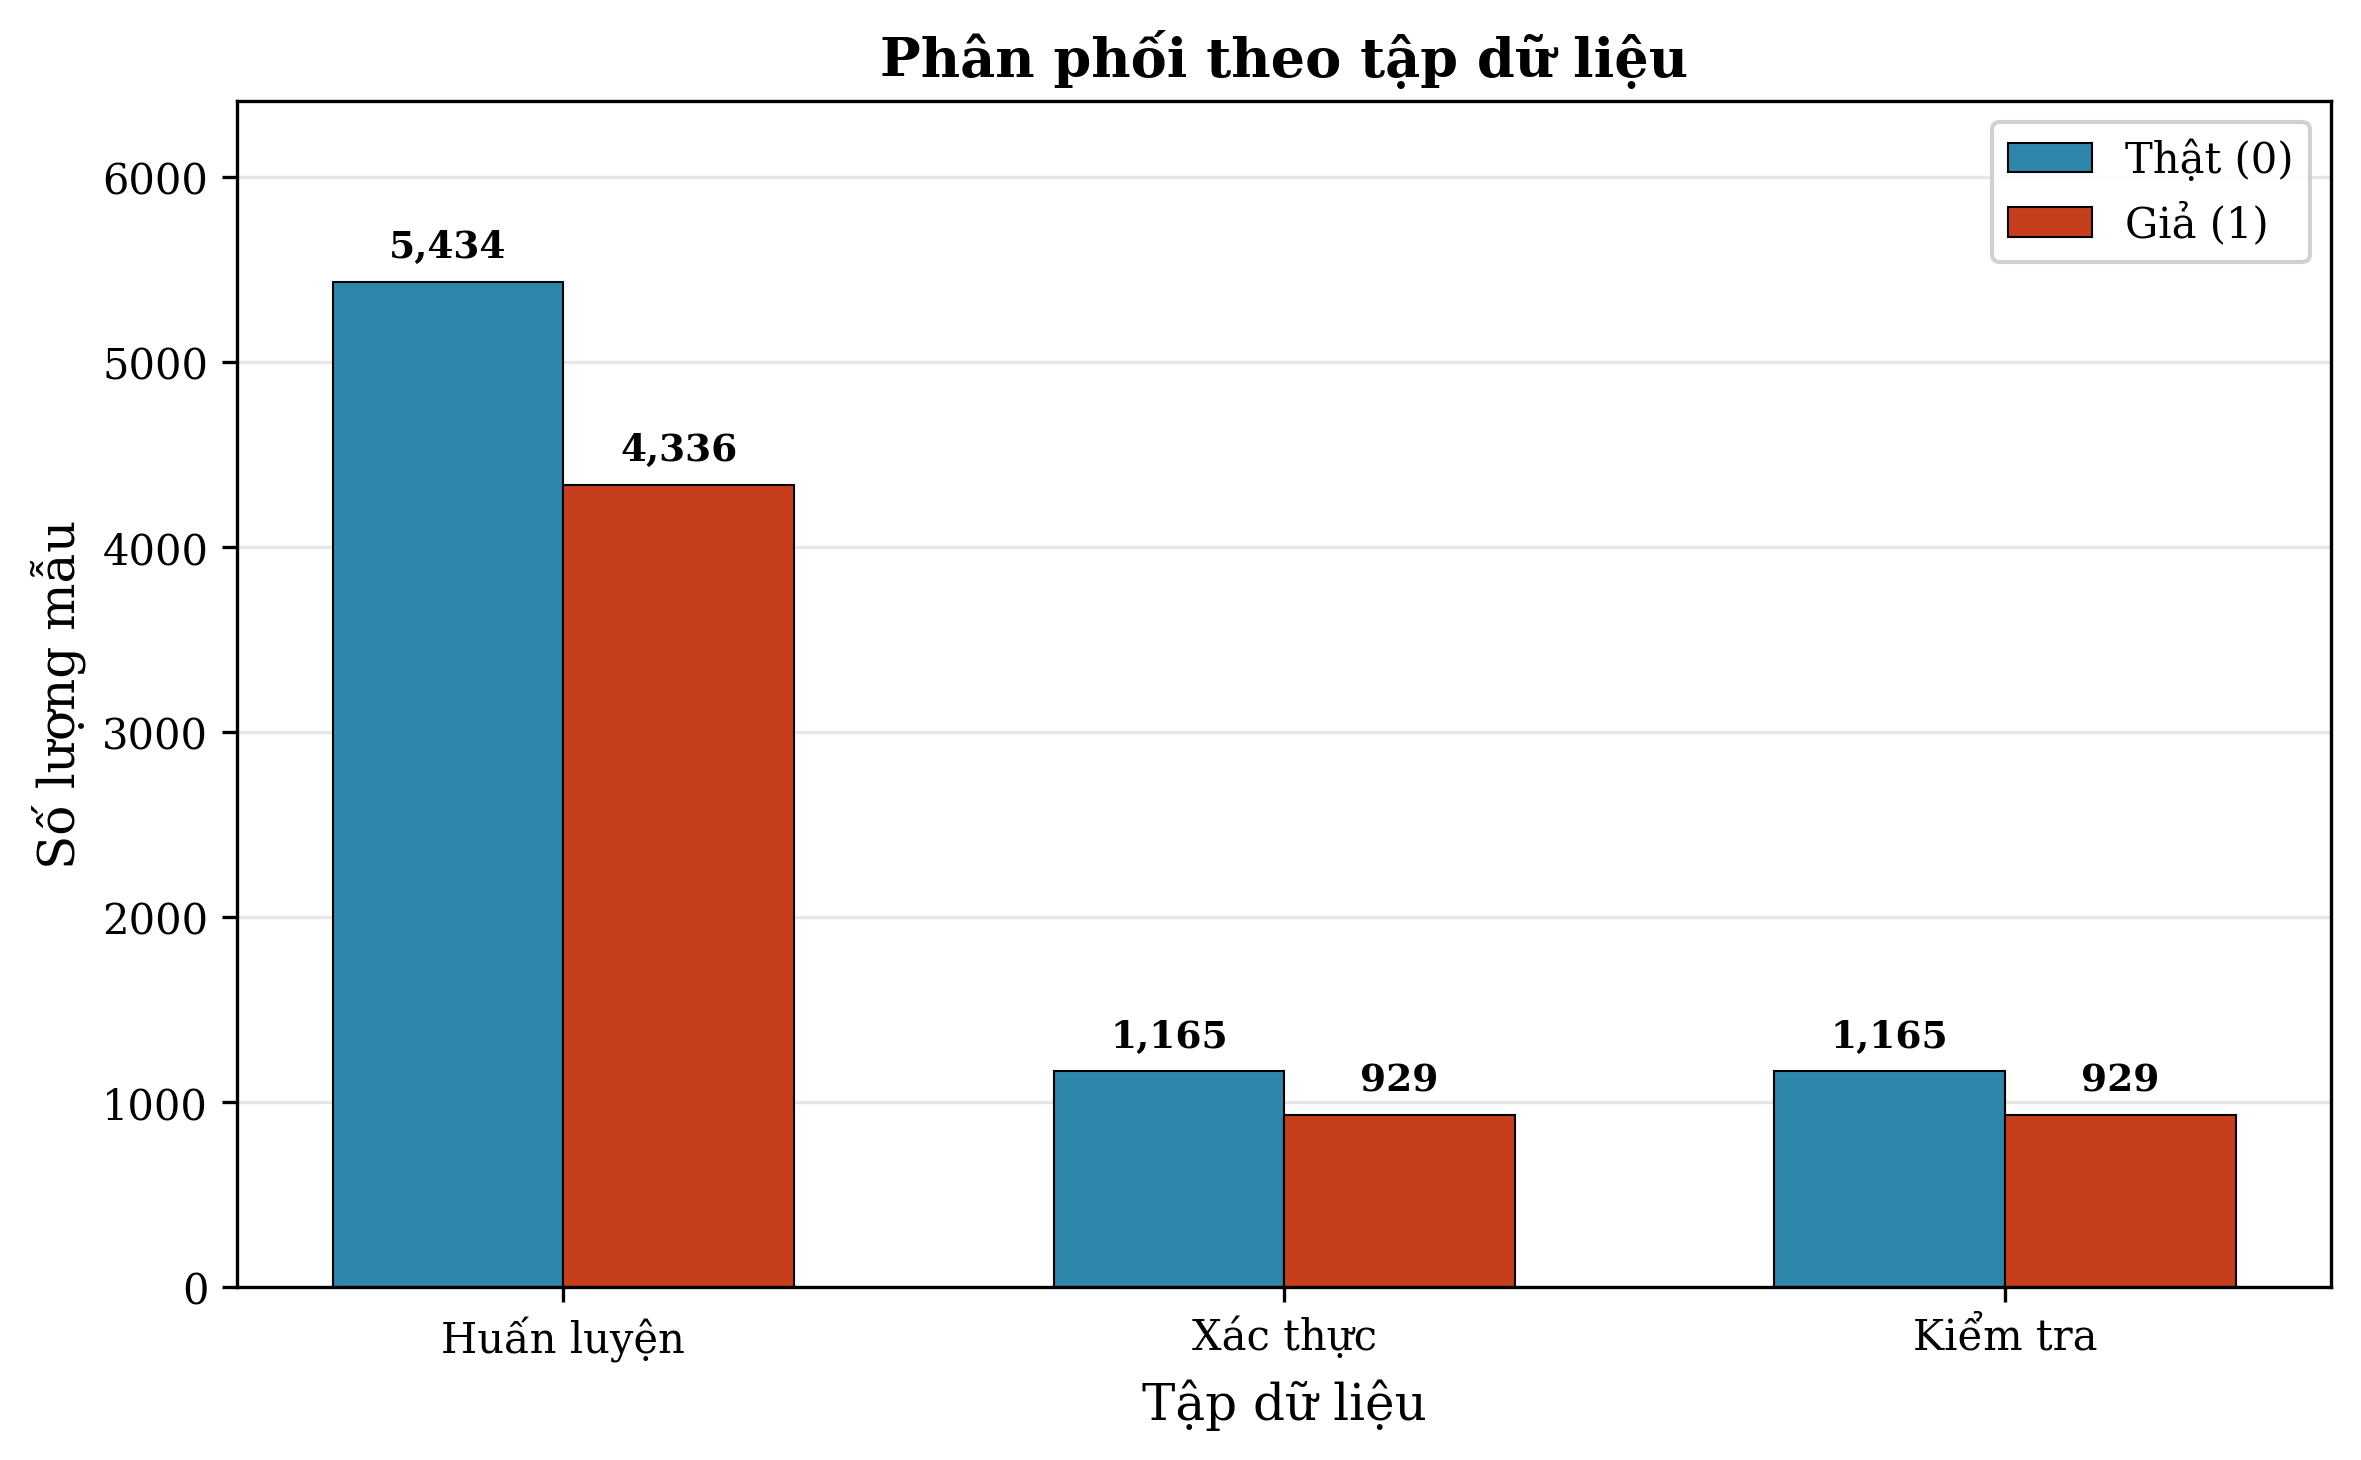
\includegraphics[width=0.92\textwidth]{fig0b_split_distribution}
  \caption{Phân phối nhãn trong các tập dữ liệu huấn luyện, kiểm định và kiểm tra}
  \label{fig:split_distribution}
\end{figure}


Bảng~\ref{tab:dataset} mô tả thống kê chi tiết sau khi chia tập:

\begin{table}[h]
\centering
\caption[Thống kê tập dữ liệu]{Thống kê tập dữ liệu}
\label{tab:dataset}
\begin{tabular}{lcccc}
\toprule
tập & tổng & \textit{tin thật} & \textit{tin giả} & độ dài tb \\
\midrule
huấn luyện & \ntrain & \ntrainreal (\pctreal\%) & \ntrainfake (\pctfake\%) & \avglentrain \\
xác thực & \nval & \nvalreal (\pctreal\%) & \nvalfake (\pctfake\%) & \avglenval \\
kiểm tra & \ntest & \ntestreal (\pctreal\%) & \ntestfake (\pctfake\%) & \avglentest \\
\bottomrule
\end{tabular}
\end{table}

Bảng~\ref{tab:dataset} thể hiện số lượng mẫu, số lượng phân phối nhãn và chiều dài trung bình của văn bản trong các tập dữ liệu. Có thể thấy, các văn bản thực và giả trong các tập huấn luyện, kiểm định và kiểm tra đều có số phần trăm tương ứng là \pctReal\% và \pctFake\%, cho thấy chiến lược chia dữ liệu theo phương pháp phân tầng (\textit{stratified split}) có thể bảo toàn số phân phối nhãn ban đầu của dữ liệu. Chiều dài trung bình của văn bản trong các tập dữ liệu kiểm định và kiểm tra (\avgLenVal\ từ trong tập dữ liệu kiểm định và \avgLenTest\ từ trong tập dữ liệu kiểm tra) cao hơn nhẹ so với chiều dài trung bình của văn bản trong tập huấn luyện (\avgLenTrain\ từ), cho thấy đa dạng cấu trúc văn bản trong các dữ liệu. Mặc dù có sự mất cân bằng lớp vừa phải trong các văn bản, số phần trăm này không quá nghiêm trọng và có thể xử lý theo cơ chế trọng số lớp (\textit{class weighting}) trong quá trình huấn luyện để giảm thiểu sai lệch dự đoán.

\subsection{Kiểm tra rò rỉ dữ liệu}
Để đảm bảo tính khách quan và độ tin cậy của quá trình đánh giá, nhóm thực hiện bước kiểm tra hiện tượng rò rỉ dữ liệu (\textit{data leakage}) giữa các tập huấn luyện, kiểm định và kiểm tra sau khi thực hiện bước chia dữ liệu.

Cụ thể, toàn bộ nội dung văn bản trong từng tập (Train, Validation, Test) được chuyển đổi thành các tập hợp (\textit{set}) dựa trên giá trị của trường \texttt{text}. Sau đó, phép giao được thực hiện giữa từng cặp tập dữ liệu để tìm ra các bản ghi trùng lặp:

\begin{itemize}
    \item Train và Validation
    \item Train và Test
    \item Validation và Test
\end{itemize}

Kết quả cho thấy:

\[
\text{Train} \cap \text{Validation} = \varnothing
\]
\[
\text{Train} \cap \text{Test} = \varnothing
\]
\[
\text{Validation} \cap \text{Test} = \varnothing
\]

Trước khi tiến hành kiểm tra rò rỉ dữ liệu, cần lưu ý rằng vấn đề này đặc biệt quan trọng trong các bài toán phân loại văn bản. Sự xuất hiện của mẫu trùng lặp giữa tập dữ liệu huấn luyện và tập dữ liệu kiểm tra có thể dẫn đến đánh giá thiên lệch (\textit{biased evaluation}). Trong trường hợp đó, năng suất cao của mô hình có thể đạt được một cách giả tạo nhờ ``ghi nhớ" nội dung của tập dữ liệu tập huấn, thay vì thực sự học được đặc trưng có khả năng tổng quát hóa.

\section{Kết luận chương}

Chương này đã trình bày quy trình hoàn chỉnh trong việc chuẩn bị dữ liệu cho bài toán 
phát hiện tin giả tiếng Việt. Các khâu trong quy trình này bao gồm khâu phân đoạn 
từ, khâu làm sạch dữ liệu, và khâu phân tập dữ liệu bằng chiến lược phân tầng. 
Dữ liệu được phân đoạn bằng thư viện RDRSegmenter để có khả năng tương thích với 
mô hình PhoBERT. Sau đó là khâu lọc bỏ dữ liệu có nội dung văn bản lặp đi lặp lại, 
rỗng hoặc quá ngắn để có thể tăng chất lượng đầu vào cho bài toán. 

Sau đó là khâu phân tập dữ liệu với tỷ lệ 70\%–15\%–15\% cho tập huấn luyện, tập 
kiểm định, tập kiểm tra của dữ liệu với \texttt{random\_state = 42}. Trong quá trình 
phân tập dữ liệu này, quy trình này sẽ thực hiện kiểm tra rò rỉ dữ liệu giữa tập huấn 
luyện và tập kiểm định để đảm bảo không tồn tại giao nhau về nội dung văn bản. 
Quy trình này đảm bảo tính nhất quán, khách quan và khả năng tái lập (\textit{reproducibility}).

\clearpage
% ============================================================
%  CHƯƠNG 3 -- PHƯƠNG PHÁP ĐỀ XUẤT
% ============================================================

\chapter{Xác định tin giả }

Trong chương này, sau phần trình bày một số lời giới thiệu về bài toán phát hiện tin giả tiếng Việt cũng như các ý tưởng trong việc tiếp cận bài toán này của nhóm, một số phương pháp trích chọn đặc trưng thủ công, cũng như các mô hình học sâu được áp dụng, bao gồm các mô hình truyền thống và các mô hình ngôn ngữ tiền huấn luyện, sẽ được trình bày thông qua lịch sử hình thành và nguyên lý của chúng.

\section{Phương pháp đề xuất}

Bài toán phát hiện tin giả được xem là một trong những bài toán quan trọng trong lĩnh vực xử lý ngôn ngữ tự nhiên, giữ vai trò rất quan trọng trong bối cảnh thông tin trực tuyến đang phát triển mạnh mẽ. Sự lan truyền nhanh chóng của các nội dung sai lệch có thể ảnh hưởng tiêu cực đến nhận thức của xã hội. Vì vậy, việc luôn luôn nghiên cứu và hoàn thiện các phương pháp phát hiện tin giả được xem là điều cần thiết. 

Cho tới nay, nhiều kỹ thuật trích xuất đặc trưng văn bản đã được các nhà nghiên cứu đề xuất và áp dụng hiệu quả, ví dụ như \textit{Bag-of-Words}, \textit{TF-IDF}~\cite{sparkjones1972idf} hay các kỹ thuật biểu diễn dựa trên word embedding~\cite{mikolov2013word2vec}. Ngoài ra, các mô hình học sâu, đặc biệt là các mạng nơ-ron hồi tiếp và các mô hình ngôn ngữ tiền huấn luyện như \textit{Transformer}~\cite{vaswani2017attention} cũng đã thể hiện được tính vượt trội của mình với những kết quả rất hứa hẹn.

Vì vậy, để có thể lựa chọn phương pháp thích hợp và hiệu quả nhất cho bài toán phát hiện tin giả tiếng Việt, nhóm quyết định thực hiện so sánh hiệu năng của các phương pháp trích chọn đặc trưng thủ công cùng các phương pháp truyền thống và hiện đại như các mô hình học sâu. Đối với các phương pháp trích chọn đặc trưng thủ công, nhóm thực hiện các thuật toán phân lớp như \textit{Logistic Regression}, \textit{SVM}, các mô hình học sâu như \textit{BiLSTM}, \textit{PhoBERT},...


\section{Lý do lựa chọn các nhóm mô hình}
\label{sec:model_selection}

Trong bài toán phân loại văn bản, đặc biệt là phát hiện tin giả,
việc lựa chọn mô hình cần cân bằng giữa ba yếu tố chính:

\begin{itemize}
    \item \textit{Khả năng diễn giải} của mô hình
    \item \textit{Chi phí tính toán}
    \item \textit{Năng lực biểu diễn ngữ nghĩa}
\end{itemize}

Dựa trên các tiêu chí này, nghiên cứu so sánh hai nhóm phương pháp chính:

\begin{enumerate}
    \item \textbf{Nhóm học máy truyền thống}

    Bao gồm:
    \begin{itemize}
        \item Logistic Regression
        \item Support Vector Machine
    \end{itemize}

    Đầu vào của các mô hình này là đặc trưng TF-IDF~\cite{sparkjones1972idf}.
    Hai mô hình có nền tảng lý thuyết vững chắc, hoạt động ổn định trên dữ
    liệu văn bản có đặc trưng chiều cao và thưa, đồng thời thuận lợi cho việc
    phân tích đóng góp của đặc trưng và kiểm soát hiện tượng quá khớp
    ~\cite{cortes1995svm}.

    Vì vậy, chúng được sử dụng như các \textit{strong baselines} nhằm đánh
    giá mức cải thiện thực sự của các phương pháp phức tạp hơn.

    \item \textbf{Nhóm học sâu}

    Bao gồm:
    \begin{itemize}
        \item BiLSTM
        \item PhoBERT
    \end{itemize}

    \textbf{BiLSTM} kế thừa khả năng ghi nhớ phụ thuộc dài hạn của
    LSTM~\cite{hochreiter1997lstm}. Khi kết hợp với cơ chế attention,
    mô hình có thể tập trung vào các thành phần thông tin quan trọng
    trong chuỗi văn bản~\cite{bahdanau2015attention}.

    \textbf{PhoBERT} là mô hình ngôn ngữ tiền huấn luyện dành riêng cho
    tiếng Việt, được xây dựng trên nền tảng Transformer/RoBERTa
    ~\cite{vaswani2017attention,liu2019roberta,phobert2020}. Mô hình này
    cho phép khai thác ngữ cảnh hai chiều ở mức sâu và thường đạt hiệu
    năng cao trong các tác vụ phân loại tiếng Việt.
\end{enumerate}

Việc đặt hai nhóm mô hình trong cùng một khung thực nghiệm giúp trả lời
ba câu hỏi nghiên cứu chính:

\begin{enumerate}
    \item Mức độ cạnh tranh của các mô hình truyền thống khi đặc trưng
    được thiết kế tốt.
    \item Lợi ích biên của học biểu diễn ngữ cảnh sâu so với đặc trưng
    TF-IDF.
    \item Giá trị gia tăng của tiền huấn luyện tiếng Việt (PhoBERT)
    đối với bài toán phát hiện tin giả trong điều kiện dữ liệu thực tế.
\end{enumerate}
\section{Tổng quan kiến trúc hệ thống}

Hệ thống được thiết kế theo ba giai đoạn chính:

\begin{enumerate}[leftmargin=3.3em]
  \item \textbf{Tiền xử lý}: Dữ liệu được làm sạch để loại bỏ các ký tự không mong muốn, đồng thời áp dụng phân đoạn từ cho tiếng Việt. Cuối cùng, dữ liệu được chia thành dữ liệu huấn luyện, kiểm định và kiểm tra với tỷ lệ tương ứng để có được kết quả khách quan trong phần đánh giá.

  \item \textbf{Trích xuất đặc trưng:} Nhóm áp dụng một số phương pháp biểu diễn văn bản khác nhau cho từng mô hình. Cụ thể, nhóm áp dụng phương pháp \textit{TF-IDF} cho hai mô hình là \textit{Logistic Regression} và \textit{SVM}; phương pháp \textit{Word Embedding} (FastText) cho mô hình \textit{BiLSTM}; phương pháp mã hóa \textit{BPE} (\textit{Byte-Pair Encoding}) cho mô hình \textit{PhoBERT} để khai thác thông tin ngữ cảnh ở mức độ sâu.

  \item \textbf{Phân loại:} Bốn mô hình là \textit{Logistic Regression}, \textit{SVM}, \textit{BiLSTM}, \textit{PhoBERT} được huấn luyện riêng biệt và đánh giá với các tiêu chí là \textit{Accuracy}, \textit{F1-score}, \textit{ROC-AUC}. Dựa trên kết quả thu được, nhóm so sánh và phân tích được hiệu năng của từng phương pháp.
\end{enumerate}

\section{Trích xuất đặc trưng}

\subsection{TF-IDF cho mô hình học máy truyền thống}

\subsubsection{Lý do lựa chọn TF-IDF}

Trong các bài toán phân loại văn bản, TF-IDF có thể được coi như một phương pháp biểu diễn đặc trưng cơ bản nhưng hiệu quả, đặc biệt là khi sử dụng kèm với các mô hình phân loại tuyến tính như Hồi quy Logistic (Logistic Regression) và Máy vectơ hỗ trợ (Support Vector Machine). Phương pháp này biểu diễn văn bản dưới dạng các vector thưa (\textit{sparse vectors}), trong đó mỗi chiều thể hiện mức độ quan trọng của một từ trong văn bản so với toàn bộ tập dữ liệu.

Cũng như nhiều phương pháp biểu diễn khác, mặc dù các phương pháp biểu diễn hiện đại như nhúng từ (\textit{word embedding}) và các mô hình Ngôn ngữ tiền huấn luyện có thể khai thác hiệu quả ngữ nghĩa sâu hơn, thì TF-IDF vẫn rất được ứng dụng trong nhiều nghiên cứu về phân loại văn bản. Cụ thể hơn, đối với các mô hình tuyến tính, biểu diễn TF-IDF có thể khai thác hiệu quả tín hiệu từ vựng (\textit{lexical cues}) có độ phân biệt cao.

Trong trường hợp bài toán phát hiện tin giả, các cụm từ giật tít, các mẫu ngôn ngữ gây chú ý hoặc các từ khóa đặc trưng thường đóng một vai trò quan trọng trong việc phân biệt tin thật và tin giả. Các tín hiệu này có thể nắm bắt một cách hiệu quả bằng các đặc trưng n-gram của TF-IDF. Vậy là TF-IDF đã có thể kết hợp với Logistic Regression và SVM như một baseline mạnh để so sánh với các phương pháp học sâu trong nghiên cứu này.

\subsubsection{Cấu hình TF-IDF}

Để đảm bảo hiệu quả biểu diễn đặc trưng cho các mô hình học máy truyền
thống, cấu hình TF-IDF được lựa chọn dựa trên kết quả \textit{ablation
study} (Mục~\ref{sec:ablation}) nhằm tối ưu hóa hiệu năng phân loại.
Cụ thể, các siêu tham số được xác định như sau:

\begin{itemize}[leftmargin=2em]

  \item \textbf{Kích thước từ điển:}
  Số lượng đặc trưng được giới hạn ở \tfidfMaxFeatures{} từ/ngữ phổ
  biến nhất. Điều này giúp giảm thiểu nhiễu và kiểm soát được sự phức tạp
  của mô hình.

  \item \textbf{N-gram:}
  Kết hợp giữa unigram và bigram (n-gram = (1, 2)) nhằm khai thác tối
  ưu cả thông tin ngữ nghĩa đơn lẻ và thông tin ngữ nghĩa lặp tiếp. Từ đó,
  nâng cao khả năng nhận diện được ngữ cảnh đặc trưng của tin giả.

  \item \textbf{Tần số tài liệu:}
  Những từ quá ít (\texttt{min\_df=5}) và quá phổ biến (\texttt{max\_df=0.95})
  đều bị loại khỏi danh sách đặc trưng. Như vậy, chỉ giữ lại danh sách đặc
  trưng có giá trị phân biệt cao.

  \item \textbf{TF sublinear:}
  Dựa trên phép biến đổi \[\text{TF} = 1 + \log f_{t,d}\] nhằm giảm bớt
  ảnh hưởng của sự lặp lại về mặt ngữ nghĩa. Điều này nhằm ưu tiên sự hiện
  diện của từ hơn là tần số tuyệt đối.

\end{itemize}

Việc lựa chọn các tham số này được thực hiện một cách hệ thống nhằm cân
bằng giữa khả năng biểu diễn đặc trưng và nguy cơ quá khớp, đồng thời
đảm bảo tính tổng quát hóa của mô hình trên các tập dữ liệu kiểm định
và kiểm tra.

\subsection{Nhúng từ (Word Embedding) cho BiLSTM}

Để phục vụ cho mô hình BiLSTM, biểu diễn văn bản được thực hiện thông qua kỹ thuật nhúng từ (word embedding) kết hợp giữa embedding tiền huấn luyện và học từ dữ liệu. Từ điển được xây dựng dựa trên toàn bộ tập train, loại bỏ các từ xuất hiện dưới 2 lần nhằm giảm nhiễu và kiểm soát kích thước không gian từ vựng, kết quả thu được \textbf{\bilstmVocab{}} từ.

Hai token đặc biệt được bổ sung: \texttt{<PAD>} (index 0) dùng để đệm các chuỗi ngắn và \texttt{<UNK>} (index 1) đại diện cho các từ ngoài từ điển. Mỗi văn bản sau tiền xử lý được chuyển đổi thành một chuỗi số nguyên với độ dài tối đa \bilstmMaxSeq, đảm bảo tính nhất quán về kích thước đầu vào cho mô hình tuần tự.

Các vector embedding có chiều \bilstmEmbDim{} được khởi tạo từ bộ embedding tiền huấn luyện FastText~\cite{bojanowski2017fasttext} phiên bản tiếng Việt (\texttt{cc.vi.300.bin}). FastText sử dụng thông tin n-gram ký tự để xây dựng biểu diễn từ, cho phép xử lý hiệu quả các từ ngoài từ điển bằng cách tổng hợp vector của các n-gram thành phần. Ma trận embedding tiền huấn luyện được nạp vào lớp embedding của mô hình và tiếp tục được tinh chỉnh trong quá trình huấn luyện thông qua lan truyền ngược, cho phép mô hình điều chỉnh biểu diễn ngữ nghĩa phù hợp với nhiệm vụ phân loại tin giả. Việc kết hợp embedding tiền huấn luyện với fine-tuning giúp tận dụng tri thức ngôn ngữ học được từ ngữ liệu lớn (Common Crawl), đồng thời thích ứng tốt với đặc thù dữ liệu tiếng Việt trong miền bài toán.

\subsection{Tokenization PhoBERT (BPE)}

Quá trình mã hóa đầu vào cho PhoBERT sử dụng thuật toán Byte-Pair Encoding (BPE)~\cite{sennrich2016bpe} với từ điển gồm 64.000 subword, cho phép mô hình xử lý hiệu quả các từ ngoài từ điển và hiện tượng đa hình trong tiếng Việt. Mỗi văn bản được tiền xử lý như sau:
\begin{itemize}[leftmargin=2em]
  \item Thêm token đặc biệt \texttt{[CLS]} ở đầu và \texttt{[SEP]} ở cuối chuỗi để đánh dấu ranh giới văn bản.
  \item Chuỗi token được cắt hoặc đệm về độ dài cố định \phobertMaxSeq{} nhằm đảm bảo tính nhất quán đầu vào.
  \item Sinh \texttt{attention\_mask} để phân biệt token thực (1) và token đệm (0), hỗ trợ quá trình attention trong mô hình.
\end{itemize}
Chiến lược này giúp PhoBERT tận dụng tối đa thông tin ngữ cảnh và đảm bảo khả năng tổng quát hóa trên dữ liệu tiếng Việt đa dạng.

\section{Các mô hình phân loại}

\subsection{Các mô hình học máy truyền thống}

\subsubsection{Hồi quy Logistic}

Mô hình hồi quy Logistic sử dụng điều chuẩn L2 nhằm hạn chế quá khớp và áp dụng cơ chế cân bằng lớp (\texttt{class\_weight=`balanced'}) để xử lý mất cân bằng nhãn. Các siêu tham số được lựa chọn thông qua GridSearchCV 5-fold, đảm bảo tính khách quan và tổng quát hóa:

\begin{itemize}[leftmargin=2em]
  \item Lưới tìm kiếm: $C \in \{0.5;\ 1;\ 5;\ 10;\ 20;\ 50\}$, solver $\in \{\text{liblinear},\ \text{saga}\}$
  \item Cấu hình tối ưu: $C = \lrBestC$, solver = saga, max\_iter = 3000
\end{itemize}

Việc lựa chọn này giúp mô hình đạt hiệu năng tốt nhất trên tập kiểm định mà không bị phụ thuộc vào phân phối nhãn.

\subsubsection{Máy vectơ hỗ trợ}

Mô hình máy vectơ hỗ trợ (SVM) sử dụng LinearSVC với trọng số lớp cân bằng để giảm thiểu ảnh hưởng của mất cân bằng nhãn. Quá trình tối ưu siêu tham số được thực hiện qua GridSearchCV với 5-fold cross-validation:

\begin{itemize}[leftmargin=2em]
  \item Lưới tìm kiếm: $C \in \{0.1;\ 0.5;\ 1;\ 2;\ 5;\ 10\}$
  \item Cấu hình tối ưu: $C = \svmBestC$, LinearSVC kết hợp hiệu chuẩn xác suất Platt~\cite{platt1999calibration} (calibration)
\end{itemize}

Chiến lược này đảm bảo SVM vừa tận dụng được đặc trưng TF-IDF vừa duy trì khả năng phân biệt tốt giữa các lớp.

\subsection{Các mô hình học sâu}

Như đã phân tích ở Mục~\ref{sec:model_selection}, BiLSTM và PhoBERT được lựa chọn lần lượt
làm đại diện cho nhóm mô hình tuần tự và nhóm mô hình ngôn ngữ tiền
huấn luyện. Phần này trình bày chi tiết kiến trúc và cấu hình huấn
luyện của hai mô hình.

\subsubsection{Mạng BiLSTM}

Kiến trúc BiLSTM được thiết kế gồm các thành phần chính sau:

\begin{enumerate}[leftmargin=2.5em]
  \item \textbf{Embedding:} Ma trận embedding kích thước $(V \times \bilstmEmbDim)$, cho phép học biểu diễn ngữ nghĩa từ dữ liệu.
  \item \textbf{BiLSTM \bilstmLayers{} tầng:} Mỗi tầng có hidden\_dim=\bilstmHiddenDim{} cho hai chiều (forward/backward), tổng đầu ra mỗi bước là $2\times\bilstmHiddenDim$.
  \item \textbf{Soft Attention:} Cơ chế soft attention tính trọng số $\alpha_t$ cho từng bước thời gian, giúp mô hình tập trung vào các từ/cụm từ quan trọng.
  \item \textbf{Classifier:} Hai lớp dropout~\cite{srivastava2014dropout} (0.3) xen kẽ với các lớp tuyến tính và ReLU~\cite{nair2010relu}, giúp giảm overfitting và tăng khả năng biểu diễn phi tuyến.
\end{enumerate}

Chiến lược huấn luyện sử dụng AdamW~\cite{loshchilov2019adamw}
($\eta = 10^{-3}$, weight\_decay=$10^{-4}$), hàm mất mát CrossEntropy
có trọng số lớp để xử lý mất cân bằng, batch=64, tối đa 20 epochs với
dừng sớm (patience=5). Ngoài ra, áp dụng ReduceLROnPlateau
(factor=0.5, patience=2) để điều chỉnh tốc độ học và gradient clipping~\cite{pascanu2013gradient}
(max\_norm=1.0) nhằm đảm bảo ổn định quá trình tối ưu.

\subsubsection{Tinh chỉnh PhoBERT}

Kiến trúc PhoBERT fine-tuning gồm hai thành phần chính:

\begin{enumerate}[leftmargin=2.5em]
  \item \textbf{Encoder PhoBERT:} 12 lớp Transformer encoder, đầu ra vector \texttt{[CLS]} 768 chiều đại diện toàn cục cho văn bản.
  \item \textbf{Classifier Head:} Hai lớp Dropout (0.1) xen kẽ với Linear (768→384→2) và ReLU~\cite{nair2010relu}, giúp tăng khả năng biểu diễn phi tuyến và giảm overfitting.
\end{enumerate}

Chiến lược huấn luyện sử dụng AdamW~\cite{loshchilov2019adamw}
($\eta = 3 \times 10^{-5}$, weight\_decay=0.01), Linear Warmup (10\%),
batch=16, tối đa 8 epochs, gradient accumulation steps=4, gradient
clipping~\cite{pascanu2013gradient} (max\_norm=1.0) và dừng sớm (patience=2).

\section{Chiến lược xử lý mất cân bằng nhãn}

Mặc dù tỷ lệ nhãn trong bộ dữ liệu (\pctReal\% Thật / \pctFake\% Giả) không quá chênh lệch, sự mất cân bằng vẫn có thể ảnh hưởng đến khả năng phân loại, đặc biệt đối với lớp thiểu số (tin giả). Để giảm thiểu tác động này, nhóm áp dụng hai chiến lược bổ trợ nhau:

\begin{itemize}[leftmargin=2em]
  \item \textbf{Chia phân tầng (\textit{stratified split}):} Dữ liệu được chia thành các tập huấn luyện, kiểm định và kiểm tra theo phương pháp phân tầng, đảm bảo tỷ lệ giữa các lớp được bảo toàn đồng đều trong từng tập. Cách tiếp cận này ngăn ngừa tình trạng mô hình bị thiên lệch do sự phân bố nhãn không đều giữa các tập.
  
  \item \textbf{Trọng số lớp trong hàm mất mát (\textit{class weighting}):} Mỗi lớp $c$ được gán trọng số nghịch đảo tỷ lệ với tần suất xuất hiện:
  \[
    w_c = \frac{N}{K \cdot N_c}
  \]
  trong đó $N$ là tổng số mẫu, $K$ là số lớp và $N_c$ là số mẫu thuộc lớp $c$. Trọng số này được tích hợp trực tiếp vào hàm mất mát CrossEntropy, tăng mức phạt cho các mẫu thuộc lớp thiểu số, từ đó cải thiện recall cho lớp tin giả. Đối với các mô hình truyền thống (LR, SVM), cơ chế tương đương được thực hiện thông qua tham số \texttt{class\_weight=`balanced'} trong scikit-learn~\cite{pedregosa2011sklearn}.
\end{itemize}

Sự kết hợp hai chiến lược trên giúp đảm bảo quá trình huấn luyện và đánh giá phản ánh đúng thực tế phân phối nhãn, đồng thời giảm thiểu nguy cơ mô hình bỏ sót các trường hợp thuộc lớp thiểu số.

\section{Kết luận chương}

Chương này đã trình bày đầy đủ từ trích xuất đặc trưng đến kiến trúc và tham số huấn luyện của bốn mô hình. Thiết kế cho phép so sánh công bằng trên cùng bộ dữ liệu và cùng quy trình đánh giá. Chương sau trình bày kết quả thực nghiệm.

\clearpage
% ============================================================
%  CHƯƠNG 4 -- KẾT QUẢ THỰC NGHIỆM
% ============================================================

\chapter{Kết quả thực nghiệm}

\section{Môi trường thực nghiệm}

% TODO: Verify software version numbers — Python 3.14.2 and PyTorch 2.10
% do not exist as of 2025. Replace with actual versions used in experiments.
Thực nghiệm được thực hiện trên hệ thống: GPU NVIDIA (CUDA 12.8), RAM 32~GB, Python 3.14.2, PyTorch 2.10, Transformers 4.44, scikit-learn~\cite{pedregosa2011sklearn} 1.8.


\begin{table}[h]
\centering
\small
\setlength{\tabcolsep}{2pt}
\caption[Siêu tham số các mô hình]{Siêu tham số các mô hình}
\label{tab:hyperparams}
\begin{tabular}{ll}
\toprule
mô hình & siêu tham số \\
\midrule
Logistic Regression & C=\lrbestc, solver=saga, class\_weight=balanced, max\_iter=3000 \\
\midrule
SVM & C=\svmbestc, linearsvc, class\_weight=balanced \\
\midrule
\multirow{4}{*}{BILSTM} & Embedding dim=\bilstmembdim, hidden dim=\bilstmhiddendim \\
 & num layers=\bilstmlayers, Dropout=0{,}3 \\
 & learning rate=0{,}001, batch size=64 \\
 & early stopping patience=5 \\
\midrule
\multirow{4}{*}{PhoBERT} & pre-trained: vinai/phobert-base \\
 & max length=\phobertmaxseq, weight decay=0{,}01 \\
 & learning rate=3e-05, batch size=16 \\
 & epochs=8, warmup ratio=0{,}1 \\
\bottomrule
\end{tabular}
\end{table}


Bảng~\ref{tab:hyperparams} tóm tắt siêu tham số cuối cùng sau tối ưu hoá.


\begin{table}[h]
\centering
\caption[Độ phức tạp và thời gian huấn luyện]{Độ phức tạp và thời gian huấn luyện}
\label{tab:complexity}
\begin{tabular}{llcc}
\toprule
mô hình & loại & tham số & thời gian huấn luyện \\
\midrule
Logistic Regression & ML truyền thống & \lrParams & 1.6 s \\
SVM & ML truyền thống & \svmParams & 3 min \\
BILSTM & Học sâu & \bilstmParamCount & 5 min \\
PhoBERT & Transformer & \phobertParamCount & 1.2 h \\
\bottomrule
\end{tabular}
\end{table}


Bảng~\ref{tab:complexity} so sánh số tham số và thời gian huấn luyện giữa các mô hình.

\section{So sánh hiệu năng các mô hình}
\label{sec:model_comparison}

\subsection{Kết quả tổng thể}

\begin{figure}[H]
  \centering
  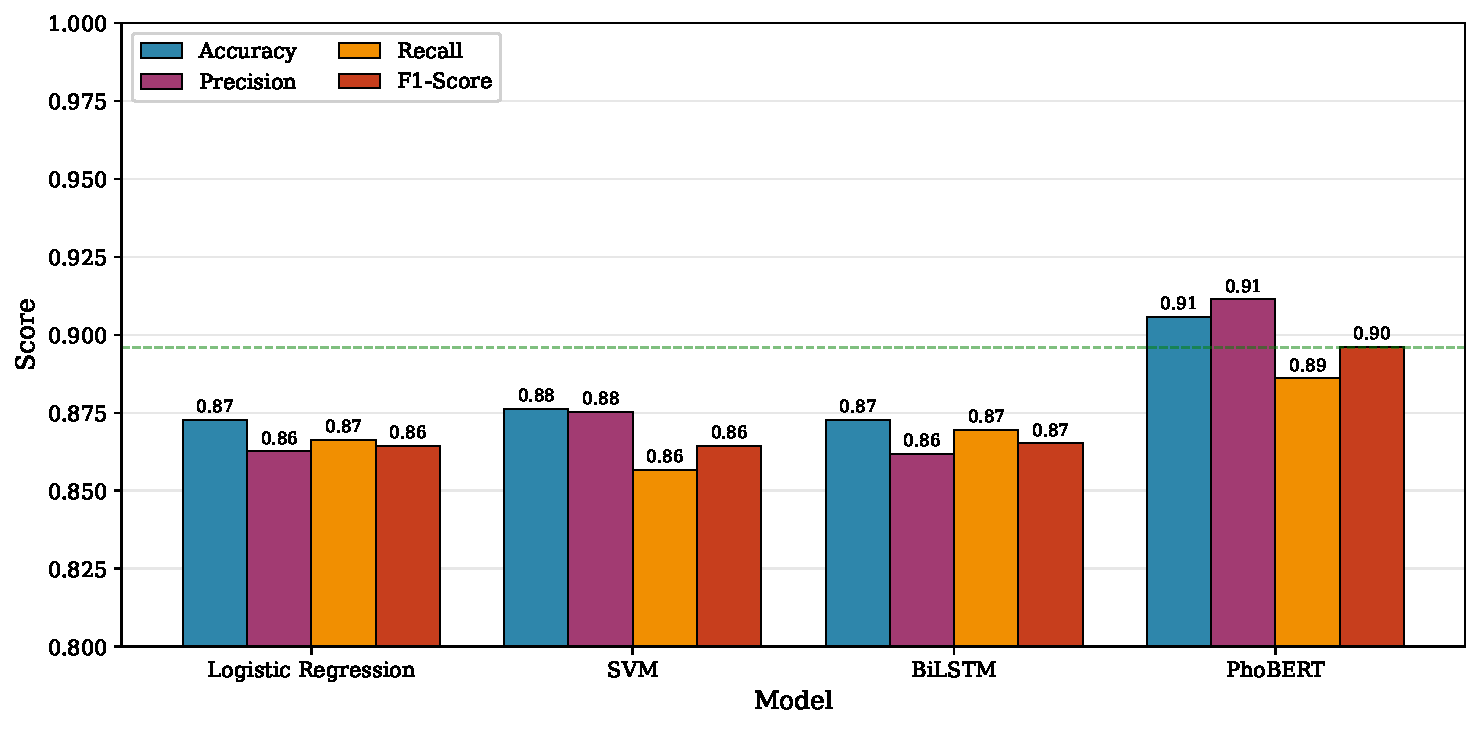
\includegraphics[width=0.92\textwidth]{fig1_model_comparison}
  \caption{So sánh các chỉ số hiệu năng (Accuracy, F1-Score, ROC-AUC) của bốn mô hình trên tập kiểm tra}
  \label{fig:model_comparison}
\end{figure}


\begin{table}[h]
\centering
\setlength{\tabcolsep}{3pt}
\small
\caption[So sánh hiệu suất các mô hình]{So sánh hiệu suất các mô hình trên tập kiểm tra}
\label{tab:results}
\begin{tabular}{lccccc}
\toprule
mô hình & độ chính xác & precision & recall & F1-Score & ROC-AUC \\
\midrule
Logistic Regression & \lrAccTab & \lrPrecTab & \lrRecTab & \lrFoneTab & \lrAUCTab \\
SVM & \svmAccTab & \svmPrecTab & \svmRecTab & \svmFoneTab & \svmAUCTab \\
BILSTM & \bilstmAccTab & \bilstmPrecTab & \bilstmRecTab & \bilstmFoneTab & \bilstmAUCTab \\
PhoBERT & \phobertAccTab & \phobertPrecTab & \phobertRecTab & \phobertFoneTab & \phobertAUCTab \\
\bottomrule
\end{tabular}
\end{table}


Bảng~\ref{tab:results} trình bày hiệu năng trên tập kiểm tra. \phobert đạt kết quả tốt nhất với \textbf{F1 = \phobertFone\%} và \textbf{AUC = \phobertAUC}, vượt trội LR (+\deltaLR\%), SVM (+\deltaSVM\%) và BiLSTM (+\deltaBiLSTM\%). Đáng chú ý, SVM vượt BiLSTM mặc dù kiến trúc đơn giản hơn, cho thấy đặc trưng TF-IDF chất lượng cao cạnh tranh được với học sâu khi dữ liệu giới hạn.

\subsection{Hiệu năng theo từng lớp}

\begin{figure}[H]
  \centering
  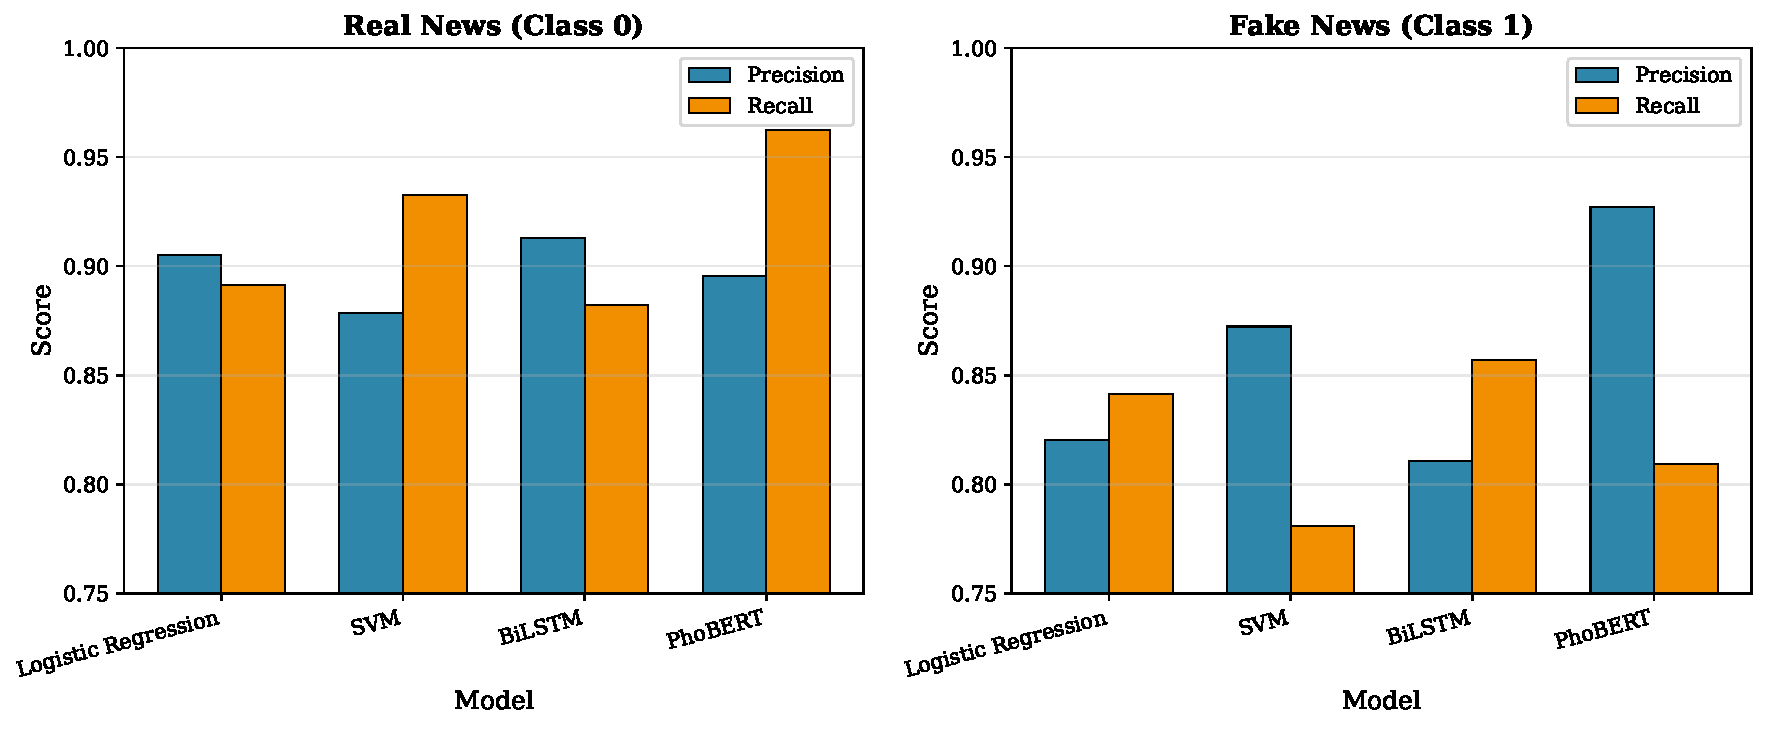
\includegraphics[width=0.92\textwidth]{fig5_per_class}
  \caption{Precision, Recall và F1-Score theo từng lớp (Thật / Giả) cho bốn mô hình}
  \label{fig:per_class}
\end{figure}


\begin{table}[h]
\centering
\caption[Chỉ số hiệu suất theo lớp]{Chỉ số hiệu suất theo từng lớp}
\label{tab:perclass}
\begin{tabular}{llccc}
\toprule
mô hình & lớp & precision & recall & F1-Score \\
\midrule
\multirow{2}{*}{Logistic Regression} & thật & \lrRealPrec & \lrRealRec & \lrRealFone \\
 & Giả & \lrFakePrec & \lrFakeRec & \lrFakeFone \\
\midrule
\multirow{2}{*}{SVM} & thật & \svmRealPrec & \svmRealRec & \svmRealFone \\
 & Giả & \svmFakePrec & \svmFakeRec & \svmFakeFone \\
\midrule
\multirow{2}{*}{BILSTM} & thật & \bilstmRealPrec & \bilstmRealRec & \bilstmRealFone \\
 & Giả & \bilstmFakePrec & \bilstmFakeRec & \bilstmFakeFone \\
\midrule
\multirow{2}{*}{PhoBERT} & thật & \phobertRealPrec & \phobertRealRec & \phobertRealFone \\
 & Giả & \phobertFakePrec & \phobertFakeRec & \phobertFakeFone \\
\bottomrule
\end{tabular}
\end{table}


Từ Bảng~\ref{tab:perclass}:
\begin{itemize}[leftmargin=2em]
  \item \phobert: Recall = \phobertRecallFake\% cho lớp Giả -- phát hiện tin giả tốt nhất trong bốn mô hình.
  \item BiLSTM: Recall = \bilstmRecallFake\% cho lớp Giả -- bỏ sót nhiều tin giả nhất (nguy hiểm trong thực tế).
  \item SVM đạt Recall = \svmRecallFake\% cho lớp Giả, cao hơn LR (\lrRecallFake\%) và BiLSTM.
\end{itemize}

\subsection{Ma trận nhầm lẫn}

\begin{figure}[H]
  \centering
  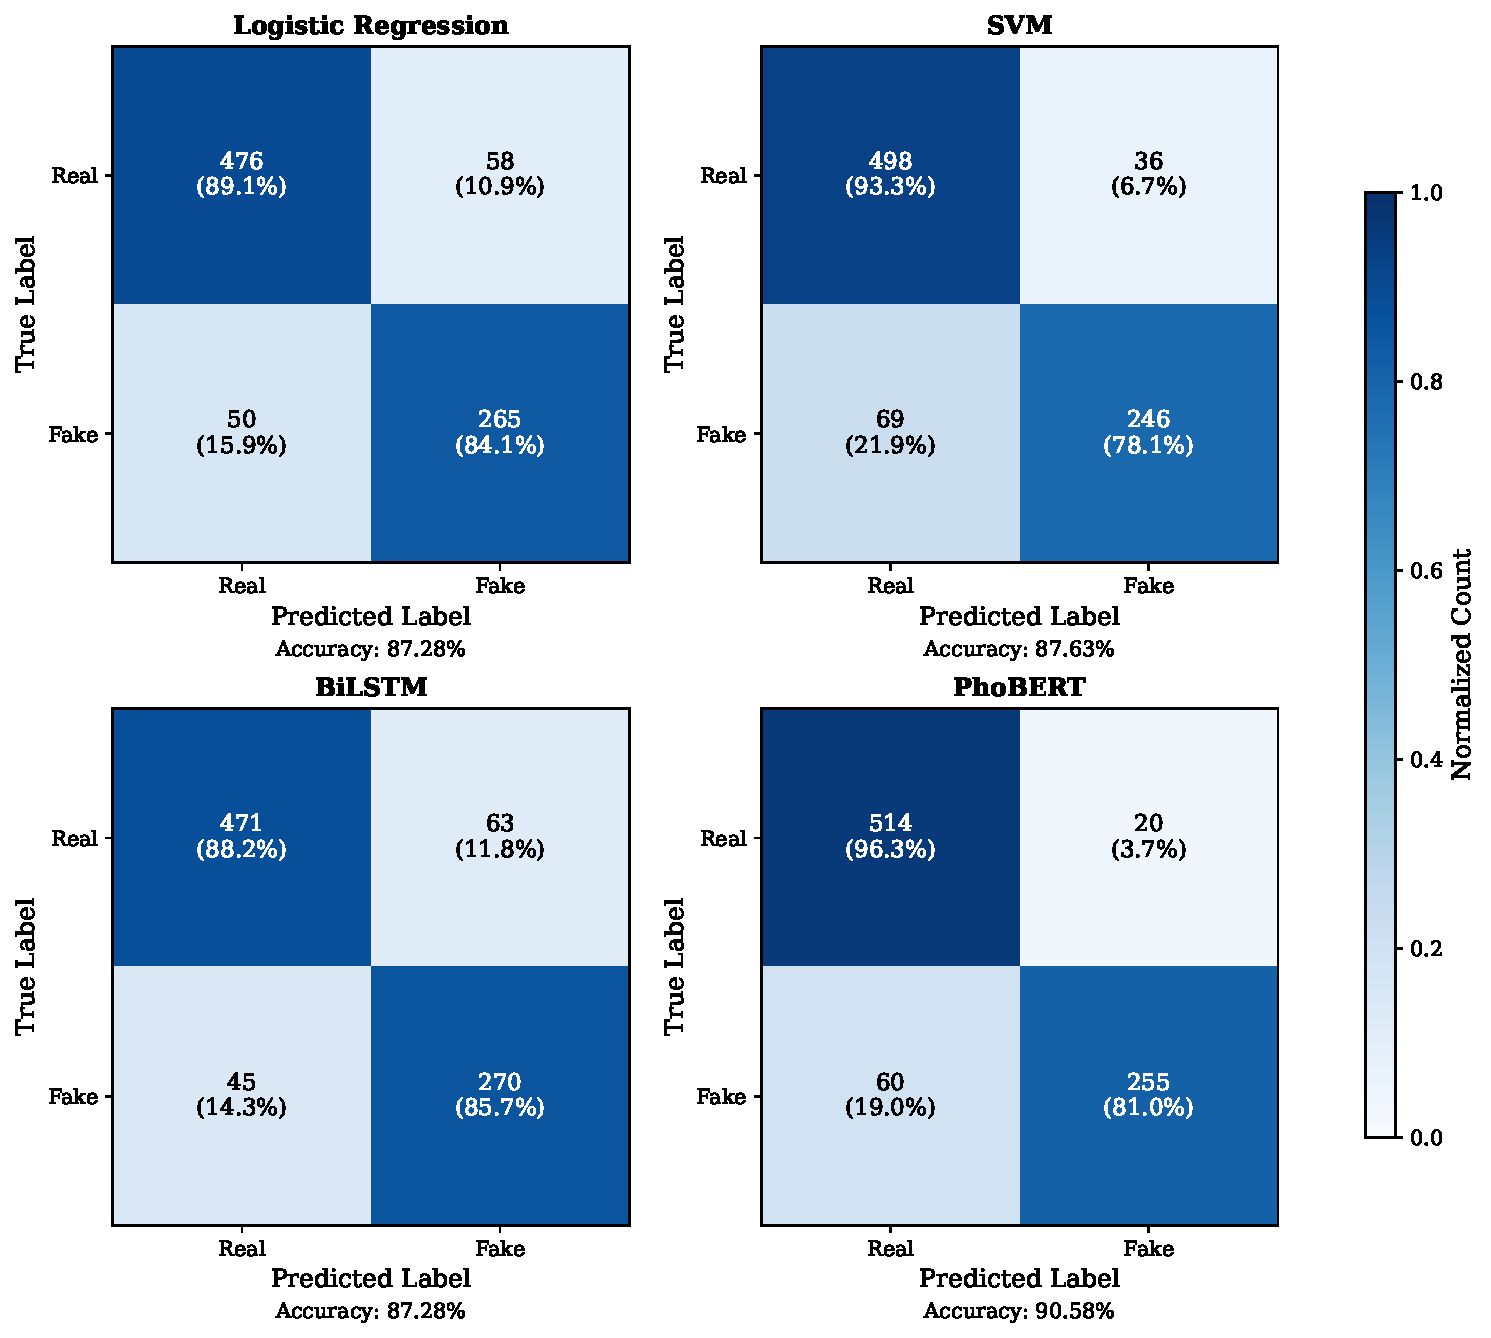
\includegraphics[width=0.95\textwidth]{fig2_confusion_matrices}
  \caption{Ma trận nhầm lẫn của bốn mô hình trên tập kiểm tra (\nTest{} mẫu)}
  \label{fig:confusion}
\end{figure}

\phobert: \phobertTN~âm tính thật (True Negative -- TN), \phobertTP~dương tính thật (True Positive -- TP), \phobertFP~dương tính giả (False Positive -- FP), \phobertFN~âm tính giả (False Negative -- FN) trên \nTest{} mẫu test. BiLSTM có nhiều lỗi nhất (\bilstmErrors~lỗi, FP=\bilstmFPcount, FN=\bilstmFNcount), trong khi \phobert ít lỗi nhất (\phobertErrors~lỗi).

\subsection{Đường cong ROC và Precision-Recall}

\begin{figure}[H]
  \centering
  \begin{subfigure}[b]{0.48\textwidth}
    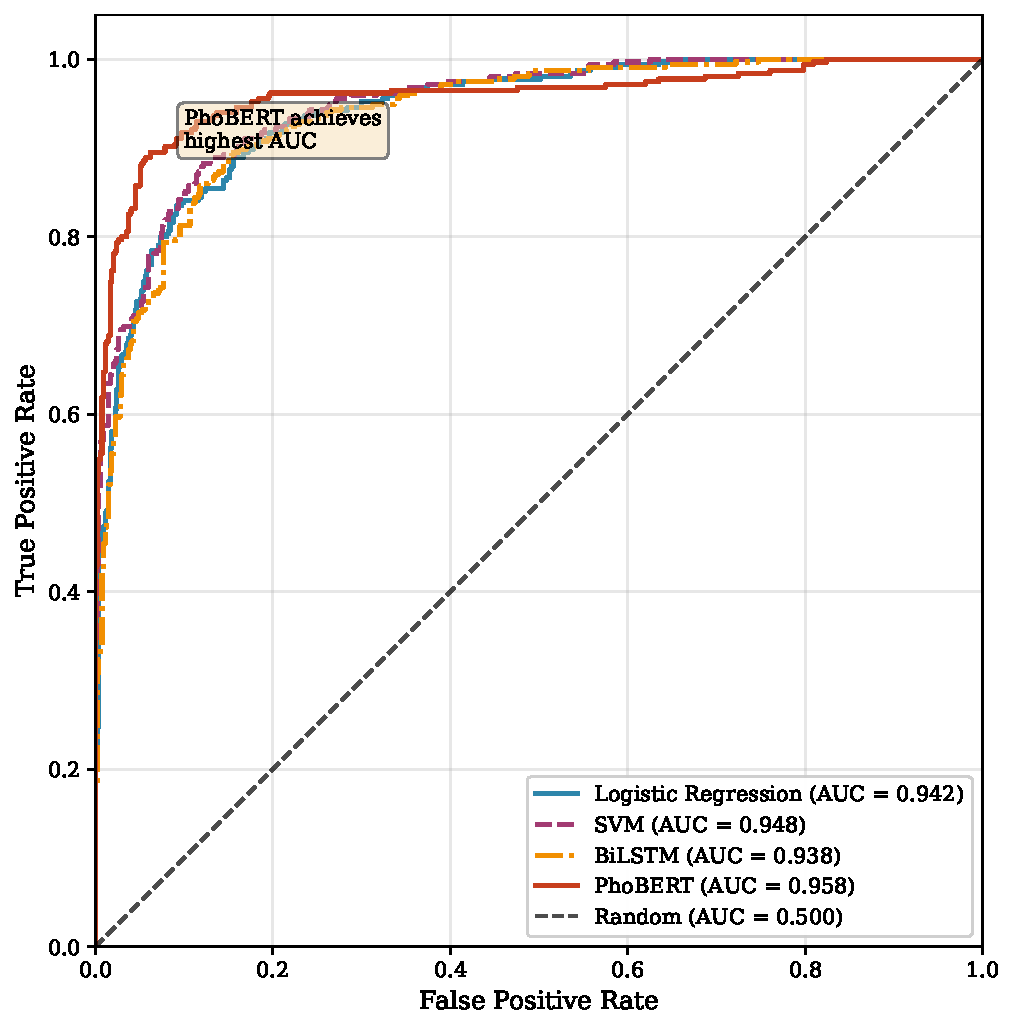
\includegraphics[width=\textwidth]{fig3_roc_curves}
    \caption{Đường cong ROC}
    \label{fig:roc}
  \end{subfigure}\hfill
  \begin{subfigure}[b]{0.48\textwidth}
    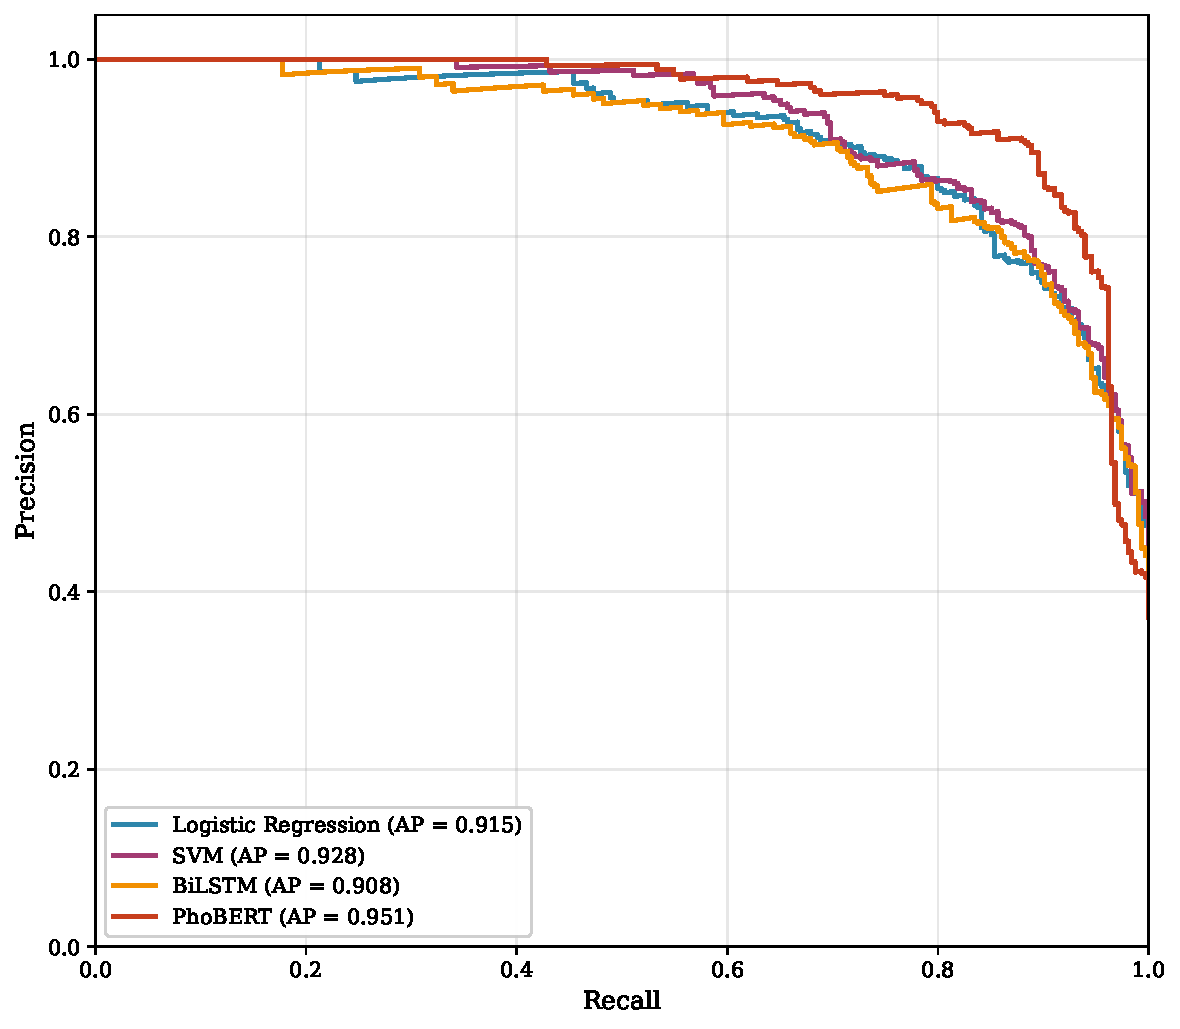
\includegraphics[width=\textwidth]{fig4_pr_curves}
    \caption{Đường cong Precision-Recall}
    \label{fig:pr}
  \end{subfigure}
  \caption{Đường cong ROC và Precision-Recall của bốn mô hình trên tập kiểm tra}
  \label{fig:curves}
\end{figure}

\phobert (AUC = \phobertAUC) áp đảo so với SVM (\svmAUC), LR (\lrAUC) và BiLSTM (\bilstmAUC).

\subsection{Phân tích hiệu chuẩn xác suất (Calibration Analysis)}
\label{sec:calibration}

Bên cạnh các chỉ số phân loại truyền thống, việc đánh giá chất lượng xác suất dự đoán của mô hình cũng đóng vai trò quan trọng trong các ứng dụng thực tế. Một mô hình được coi là có hiệu chuẩn tốt (\textit{well-calibrated}) khi xác suất dự đoán phản ánh đúng tỷ lệ dương tính thực tế: nếu mô hình dự đoán xác suất 80\% cho một nhóm mẫu, thì khoảng 80\% số mẫu đó phải thực sự thuộc lớp dương.

Điều này đặc biệt quan trọng trong bài toán phát hiện tin giả, vì người dùng hoặc hệ thống downstream cần biết mức độ tin cậy thực sự của mỗi dự đoán để quyết định hành động phù hợp (ví dụ: đánh dấu cảnh báo, chuyển sang kiểm tra thủ công, hoặc tự động loại bỏ).

Nghiên cứu sử dụng ba chỉ số đánh giá hiệu chuẩn~\cite{naeini2015ece}:

\begin{itemize}[leftmargin=2em]
  \item \textbf{Expected Calibration Error (ECE):} Sai số hiệu chuẩn kỳ vọng, đo mức chênh lệch trung bình có trọng số giữa xác suất dự đoán và tỷ lệ dương tính thực tế trên các nhóm mẫu (bin):
  \[
    \text{ECE} = \sum_{b=1}^{B} \frac{|B_b|}{N} \cdot |\text{acc}(B_b) - \text{conf}(B_b)|
  \]
  trong đó $B_b$ là tập mẫu trong bin thứ $b$, $\text{acc}(B_b)$ là tỷ lệ dự đoán đúng và $\text{conf}(B_b)$ là xác suất dự đoán trung bình trong bin đó.

  \item \textbf{Maximum Calibration Error (MCE):} Sai số hiệu chuẩn cực đại, phản ánh bin có độ lệch lớn nhất:
  \[
    \text{MCE} = \max_{b} |\text{acc}(B_b) - \text{conf}(B_b)|
  \]

  \item \textbf{Brier Score:} Trung bình bình phương sai số giữa xác suất dự đoán và nhãn thực:
  \[
    \text{BS} = \frac{1}{N} \sum_{i=1}^{N} (p_i - y_i)^2
  \]
  Brier Score kết hợp cả khả năng phân loại và hiệu chuẩn trong một chỉ số duy nhất.
\end{itemize}

Cả ba chỉ số đều có giá trị càng thấp càng tốt (0 = hoàn hảo).

\begin{figure}[H]
  \centering
  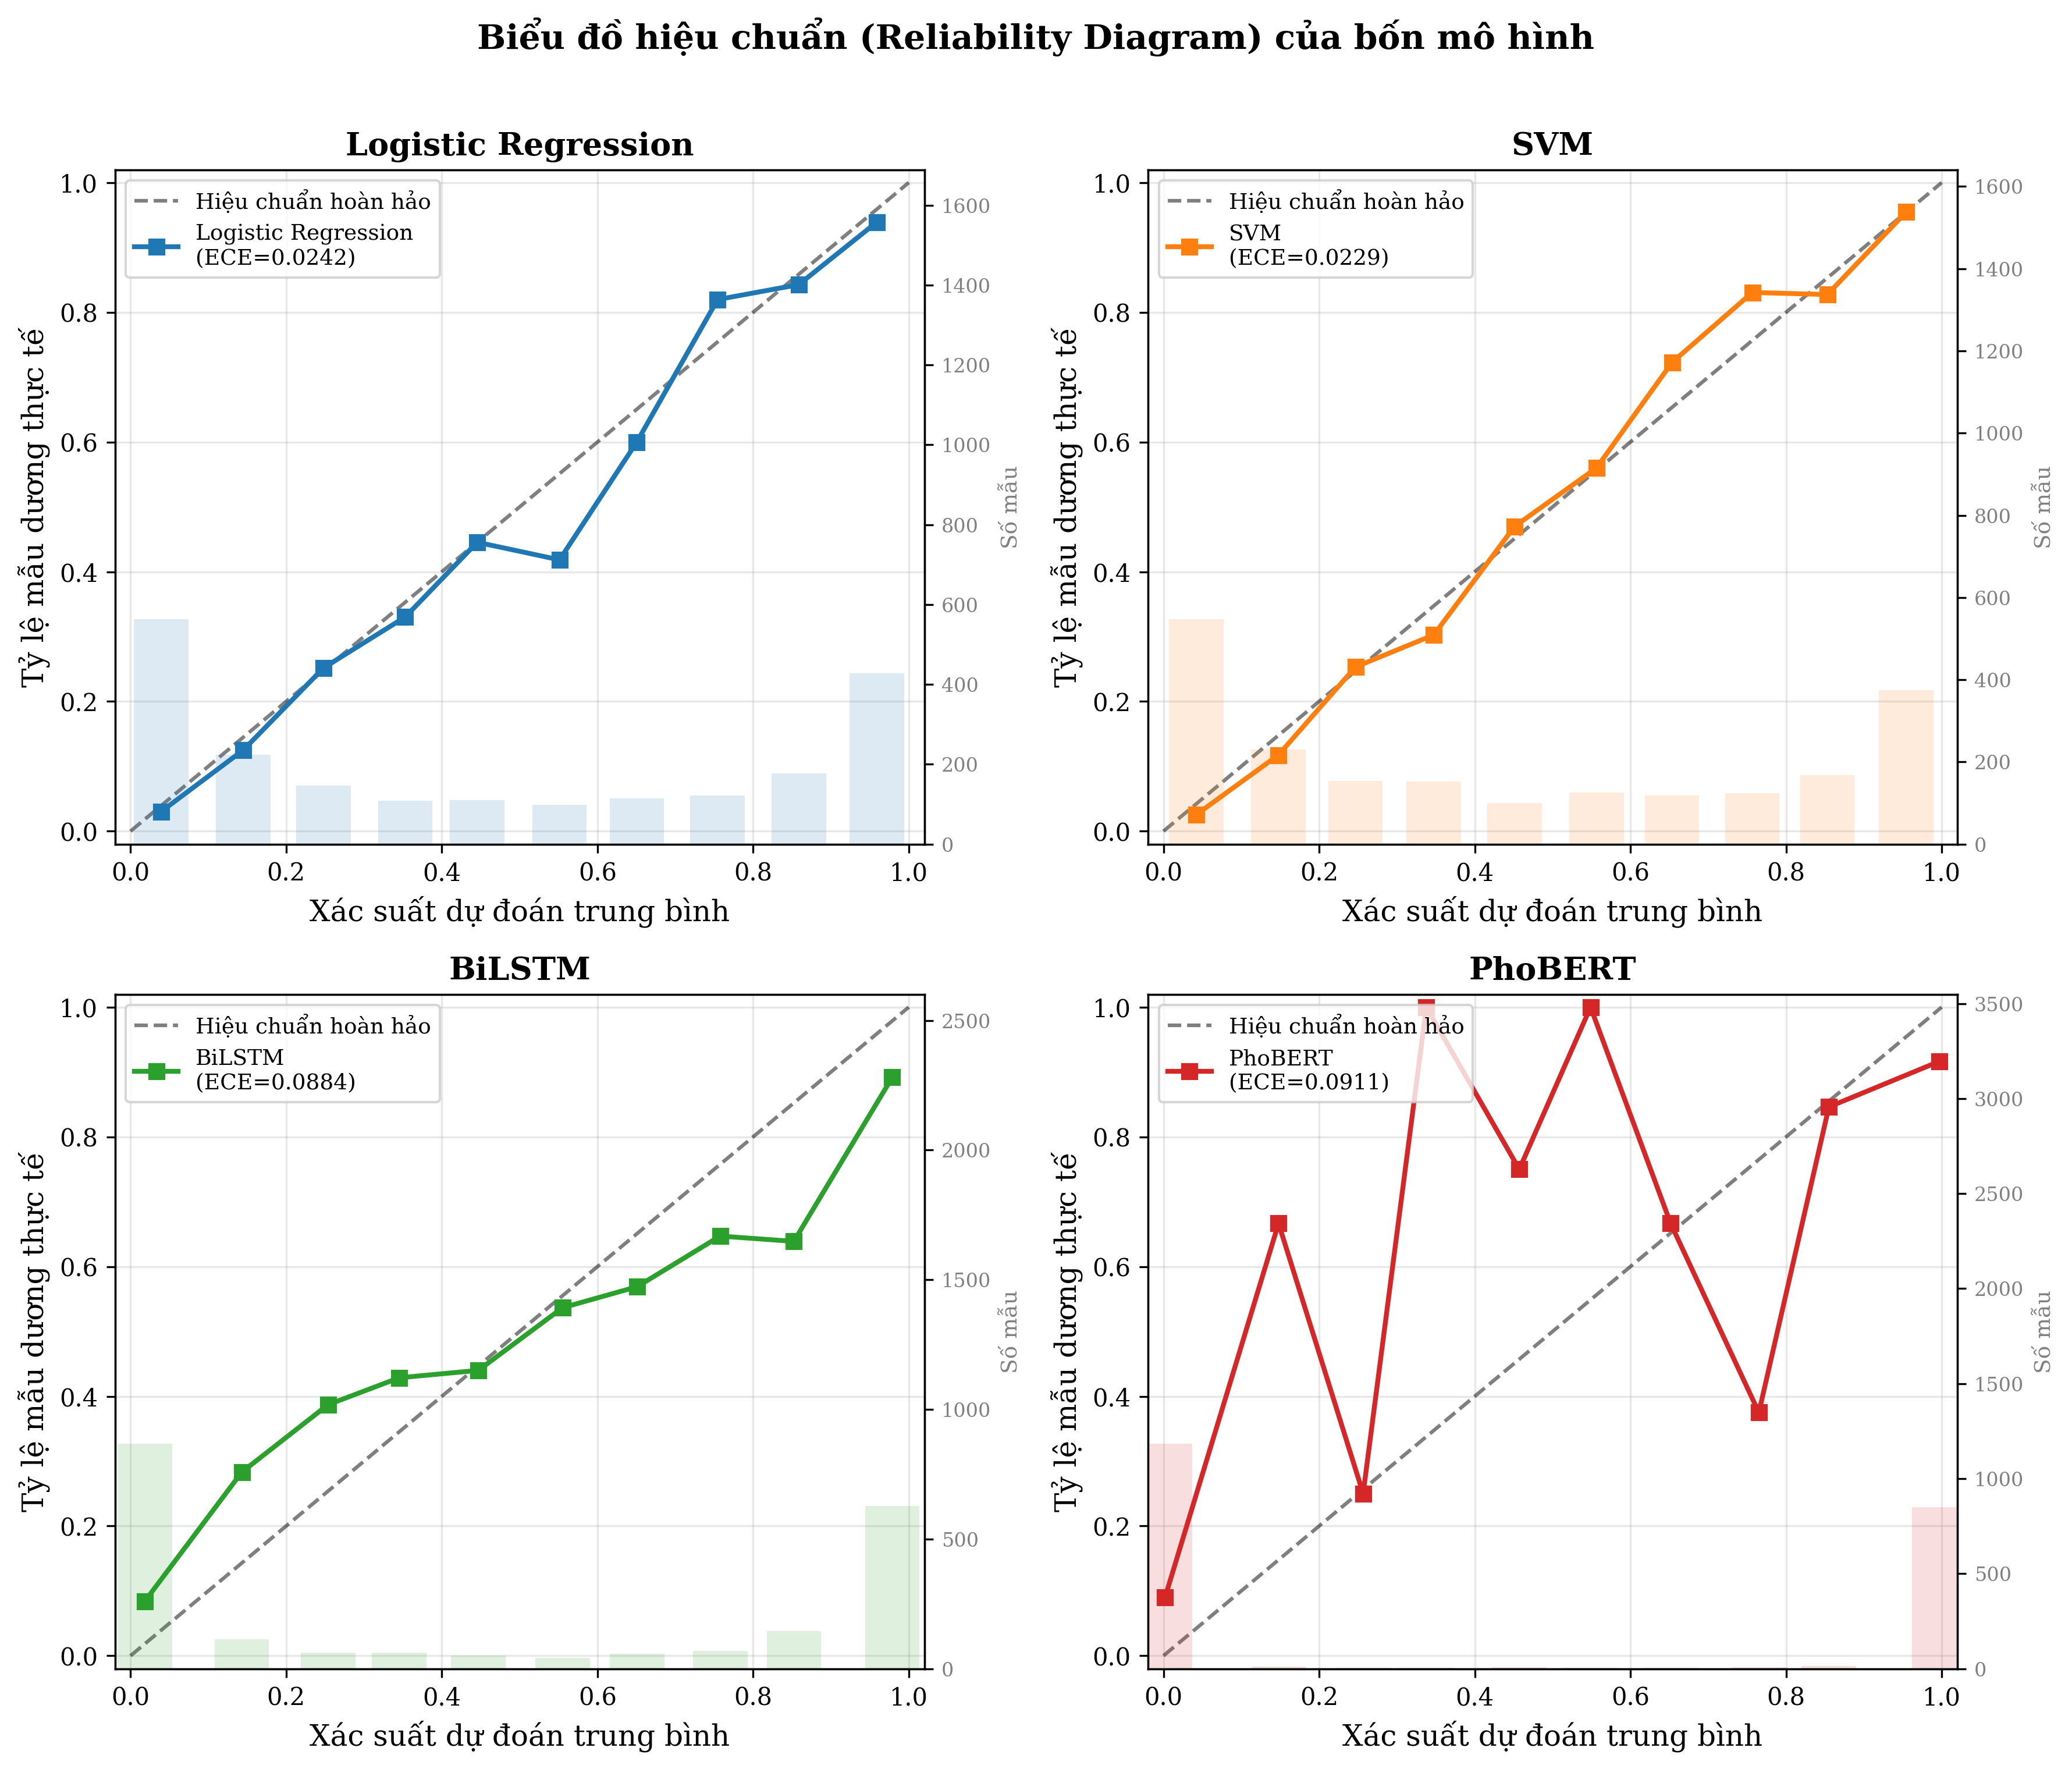
\includegraphics[width=0.95\textwidth]{fig_calibration_curves}
  \caption{Biểu đồ hiệu chuẩn (Reliability Diagram) của bốn mô hình trên tập kiểm tra. Đường chéo nét đứt biểu diễn hiệu chuẩn hoàn hảo; các điểm vuông biểu diễn tỷ lệ dương tính thực tế trong mỗi bin xác suất.}
  \label{fig:calibration}
\end{figure}

\begin{table}[H]
\centering
\caption{Chỉ số hiệu chuẩn xác suất của bốn mô hình trên tập kiểm tra}
\label{tab:calibration}
\begin{tabular}{lccc}
\toprule
\textbf{Mô hình} & \textbf{ECE} $\downarrow$ & \textbf{MCE} $\downarrow$ & \textbf{Brier Score} $\downarrow$ \\
\midrule
Logistic Regression & \lrECE & \lrMCE & \lrBrier \\
SVM & \textbf{\svmECE} & \textbf{\svmMCE} & \svmBrier \\
BiLSTM & \bilstmECE & \bilstmMCE & \bilstmBrier \\
PhoBERT & \phobertECE & \phobertMCE & \textbf{\phobertBrier} \\
\bottomrule
\end{tabular}
\end{table}

Từ Bảng~\ref{tab:calibration} và Hình~\ref{fig:calibration}, có thể rút ra một số quan sát đáng chú ý:

\begin{itemize}[leftmargin=2em]
  \item \textbf{Các mô hình học máy truyền thống có hiệu chuẩn tốt nhất:} SVM đạt ECE thấp nhất (\svmECE) và MCE thấp nhất (\svmMCE), theo sau là LR (ECE = \lrECE). Điều này cho thấy xác suất dự đoán của SVM và LR phản ánh khá chính xác tỷ lệ dương tính thực tế. Kết quả này phù hợp với lý thuyết, vì Logistic Regression được thiết kế để ước lượng xác suất trực tiếp, và SVM sử dụng hiệu chuẩn Platt~\cite{platt1999calibration} (CalibratedClassifierCV) trong quá trình huấn luyện.

  \item \textbf{PhoBERT có Brier Score tốt nhất nhưng MCE cao:} PhoBERT đạt Brier Score thấp nhất (\phobertBrier), phản ánh khả năng phân loại vượt trội. Tuy nhiên, MCE rất cao (\phobertMCE) cho thấy mô hình có xu hướng \textit{overconfident} -- đưa ra xác suất rất cao (gần 0 hoặc 1) ngay cả khi dự đoán sai. Hiện tượng này là đặc trưng phổ biến của các mô hình Transformer, đặc biệt sau quá trình fine-tuning trên tập dữ liệu nhỏ~\cite{guo2017calibration}.

  \item \textbf{BiLSTM có hiệu chuẩn kém nhất:} Với ECE = \bilstmECE\ và Brier Score = \bilstmBrier, BiLSTM cho thấy xác suất dự đoán không phản ánh tốt độ chính xác thực tế, nhất quán với hiệu năng phân loại thấp nhất trong bốn mô hình.
\end{itemize}

\textbf{Hàm ý thực tế.} Phân tích hiệu chuẩn cho thấy trong các hệ thống triển khai thực tế, \textit{không nên sử dụng trực tiếp} xác suất thô (raw probability) của PhoBERT làm mức độ tin cậy. Thay vào đó, cần áp dụng kỹ thuật hiệu chuẩn hậu xử lý (\textit{post-hoc calibration}) như Temperature Scaling~\cite{guo2017calibration} hoặc Platt Scaling~\cite{platt1999calibration} để cải thiện chất lượng xác suất trước khi đưa vào hệ thống ra quyết định. Ngược lại, xác suất từ SVM và LR có thể được sử dụng trực tiếp với độ tin cậy cao hơn.

\section{Kiểm định thống kê}
\label{sec:statistics}

\subsection{Kiểm định McNemar}

Kiểm định McNemar~\cite{mcnemar1947} được sử dụng để so sánh hiệu năng của hai mô hình phân loại trên cùng một tập kiểm thử, dựa trên các dự đoán theo từng mẫu (paired predictions). Kiểm định này đặc biệt phù hợp trong bối cảnh hai mô hình được đánh giá trên cùng dữ liệu và cần xác định liệu sự khác biệt quan sát được có mang ý nghĩa thống kê hay chỉ do ngẫu nhiên.

Giả thuyết kiểm định được thiết lập như sau:

\begin{itemize}
    \item $H_0$: Không tồn tại sự khác biệt có ý nghĩa thống kê giữa xác suất dự đoán đúng của hai mô hình.
    \item $H_1$: Tồn tại sự khác biệt có ý nghĩa thống kê giữa xác suất dự đoán đúng của hai mô hình.
\end{itemize}

Thống kê kiểm định được tính theo công thức:

$$\chi^2 = \frac{(|b - c| - 1)^2}{b + c}$$

Hai đại lượng $b$ và $c$ đại diện cho các trường hợp bất đồng (discordant pairs) giữa hai mô hình. 
Các trường hợp cả hai cùng đúng hoặc cùng sai không ảnh hưởng đến thống kê kiểm định 
vì không phản ánh sự khác biệt tương đối.

Giá trị $\chi^2$ càng lớn cho thấy mức độ chênh lệch giữa $b$ và $c$ càng cao, 
tức là sự khác biệt có xu hướng mang tính hệ thống thay vì ngẫu nhiên. 
Giá trị $p$-value được tính dựa trên phân phối Chi-square với $1$ bậc tự do. 
Nếu $p < \alpha$ (với $\alpha = 0.05$), giả thuyết $H_0$ bị bác bỏ và có thể kết luận 
sự khác biệt giữa hai mô hình là có ý nghĩa thống kê.

Hệ số điều chỉnh $(-1)$ trong tử số là hiệu chỉnh liên tục 
(\textit{continuity correction}), giúp giảm sai số loại I 
khi kích thước mẫu không quá lớn.

Do nghiên cứu thực hiện sáu phép so sánh cặp mô hình, việc tiến hành nhiều kiểm định 
đồng thời có thể làm gia tăng xác suất sai loại I. 
Để kiểm soát mức sai số toàn cục (\textit{family-wise error rate}), 
phương pháp hiệu chỉnh Holm--Bonferroni được áp dụng.

Cụ thể, các $p$-value được sắp xếp theo thứ tự tăng dần và so sánh tuần tự 
với các ngưỡng hiệu chỉnh tương ứng, bảo đảm rằng xác suất xuất hiện ít nhất 
một kết luận sai không vượt quá mức ý nghĩa $\alpha$ đã lựa chọn.

Với hiệu chỉnh Holm-Bonferroni~\cite{holm1979} cho 6 phép so sánh:

\begin{table}[H]
\centering
\caption{Kết quả kiểm định McNemar (sau hiệu chỉnh Holm-Bonferroni)}
\label{tab:mcnemar}
\begin{tabular}{llrrl}
\toprule
\textbf{Mô hình 1} & \textbf{Mô hình 2} & \textbf{$\chi^2$} & \textbf{$p$-value} & \textbf{Kết luận} \\
\midrule
LR      & SVM     & \mcnLrSvmChi  & \mcnLrSvmP    & Không có ý nghĩa \\
LR      & BiLSTM  & \mcnLrBilstmChi  & \mcnLrBilstmP    & Không có ý nghĩa \\
LR      & PhoBERT & \mcnLrPhobertChi & $<$0.001  & Có ý nghĩa (***) \\
SVM     & BiLSTM  & \mcnSvmBilstmChi  & \mcnSvmBilstmP    & Không có ý nghĩa \\
SVM     & PhoBERT & \mcnSvmPhobertChi & $<$0.001  & Có ý nghĩa (***) \\
BiLSTM  & PhoBERT & \mcnBilstmPhobertChi & $<$0.001  & Có ý nghĩa (***) \\
\bottomrule
\end{tabular}
\end{table}

\phobert vượt trội có ý nghĩa thống kê so với cả ba mô hình còn lại ($p < 0.001$). LR, SVM và BiLSTM không khác biệt đáng kể với nhau ($p \geq 0.05$ sau hiệu chỉnh Holm-Bonferroni) dù kiến trúc khác nhau hoàn toàn.

\subsection{Khoảng tin cậy Bootstrap}
Bên cạnh kiểm định McNemar, nghiên cứu tiếp tục sử dụng phương pháp 
Bootstrap nhằm ước lượng độ ổn định của chỉ số F1-score và đánh giá 
độ tin cậy của sự khác biệt giữa các mô hình.

Bootstrap là kỹ thuật lấy mẫu lặp lại có hoàn lại 
(\textit{resampling with replacement}) từ tập kiểm thử ban đầu 
để tạo ra nhiều tập mẫu giả lập. Trong nghiên cứu này, quá trình 
lấy mẫu được thực hiện 10,000 lần. Với mỗi lần lấy mẫu, 
F1-score được tính lại, từ đó xây dựng phân phối thực nghiệm 
của chỉ số này.

Khoảng tin cậy 95\% (95\% Confidence Interval -- CI) được xác định 
từ phân vị 2.5\% và 97.5\% của phân phối Bootstrap. 
Khoảng này biểu diễn miền giá trị mà tham số thực 
(F1-score kỳ vọng trên tổng thể) có khả năng nằm trong đó 
với mức tin cậy 95\%.

Việc sử dụng Bootstrap mang ý nghĩa quan trọng trong đánh giá 
thực nghiệm vì:

\begin{itemize}
    \item Không giả định phân phối chuẩn của F1-score.
    \item Phản ánh mức độ dao động của mô hình khi dữ liệu thay đổi.
    \item Cho phép so sánh mức độ chồng lấp giữa các khoảng tin cậy, 
    từ đó hỗ trợ xác nhận sự khác biệt có tính hệ thống.
\end{itemize}

Kết quả khoảng tin cậy 95\% cho các mô hình được trình bày 
trong bảng ~\ref{tab:ci}.

\begin{table}[H]
\centering
\caption{Khoảng tin cậy 95\% Bootstrap~\cite{efron1979bootstrap} cho F1-Score (10,000 lần lấy mẫu lại)}
\label{tab:ci}
\begin{tabular}{lcc}
\toprule
\textbf{Mô hình} & \textbf{F1-Score} & \textbf{95\% CI} \\
\midrule
LR      & \lrFone  & \lrFoneCI{} \\
SVM     & \svmFone & \svmFoneCI{} \\
BiLSTM  & \bilstmFone & \bilstmFoneCI{} \\
PhoBERT & \textbf{\phobertFone} & \textbf{\phobertFoneCI{}} \\
\bottomrule
\end{tabular}
\end{table}

Từ Bảng~\ref{tab:ci} có thể quan sát rằng:

\begin{itemize}
    \item PhoBERT đạt F1-score trung bình cao nhất (\phobertFone  \%)
    với khoảng tin cậy 95\% là {\phobertFoneCI{}}.
    
    \item Khoảng tin cậy của PhoBERT không chồng lấp với bất kỳ 
    mô hình nào còn lại.
    
    \item Các mô hình LR, SVM và BiLSTM có khoảng tin cậy tương đối 
    gần nhau và tồn tại hiện tượng chồng lấp.
\end{itemize}

Sự không chồng lấp khoảng tin cậy giữa PhoBERT và các mô hình khác 
củng cố kết luận từ kiểm định McNemar rằng sự vượt trội của PhoBERT 
không phải do dao động ngẫu nhiên mà mang tính ổn định thống kê. 
Ngược lại, sự chồng lấp giữa LR, SVM và BiLSTM cho thấy sự khác biệt 
hiệu năng giữa ba mô hình này chưa đủ mạnh để kết luận tồn tại 
ưu thế rõ ràng.

Như vậy, Bootstrap đóng vai trò bổ sung cho kiểm định McNemar: 
nếu McNemar kiểm tra sự khác biệt ở mức dự đoán từng mẫu 
(\textit{instance-level comparison}), thì Bootstrap đánh giá 
độ ổn định của chỉ số tổng hợp (F1-score) dưới biến thiên dữ liệu 
(\textit{metric-level stability}). Việc kết hợp cả hai phương pháp 
giúp tăng độ tin cậy và tính thuyết phục cho kết luận thực nghiệm.

\subsection{Kiểm tra chéo (Cross-Validation)}

Bên cạnh việc đánh giá trên tập kiểm thử cố định, nghiên cứu tiếp tục 
thực hiện kiểm tra chéo phân tầng (\textit{Stratified Cross-Validation}) 
nhằm đánh giá tính ổn định của mô hình dưới các cách chia dữ liệu khác nhau.

Cụ thể, phương pháp 5-fold cross-validation được áp dụng với 3 seed 
ngẫu nhiên khác nhau, tạo thành tổng cộng 15 lần huấn luyện và đánh giá. 
Việc lặp lại trên nhiều seed giúp giảm ảnh hưởng của tính ngẫu nhiên 
trong quá trình chia dữ liệu và cung cấp ước lượng ổn định hơn 
về hiệu năng trung bình.

Trong mỗi lần lặp, mô hình được huấn luyện trên 4 folds và kiểm tra 
trên fold còn lại. Các chỉ số Accuracy và F1-score được ghi nhận 
cho từng lần chạy, sau đó tính giá trị trung bình và độ lệch chuẩn.

Độ lệch chuẩn ($\pm$) phản ánh mức độ dao động của hiệu năng 
giữa các lần chia dữ liệu. Giá trị này càng nhỏ cho thấy mô hình 
càng ổn định và ít phụ thuộc vào cách phân chia tập dữ liệu.
Do hạn chế về tài nguyên tính toán và thời gian huấn luyện đáng kể của các mô hình học sâu như BiLSTM và PhoBERT, quy trình kiểm tra chéo 5-fold với 3 seed (tổng 15 lần chạy) chỉ được áp dụng cho các mô hình học máy truyền thống (Logistic Regression và SVM). Việc mở rộng quy trình này cho các mô hình học sâu sẽ đòi hỏi chi phí tính toán rất lớn và vượt quá phạm vi thực nghiệm của nghiên cứu.

Kết quả kiểm tra chéo được trình bày trong Bảng~\ref{tab:cv}.

\begin{table}[H]
\centering
\caption{Kết quả kiểm tra chéo 5-fold (3 seeds)}
\label{tab:cv}
\begin{tabular}{lcc}
\toprule
\textbf{Mô hình} & \textbf{Accuracy} & \textbf{F1-Score} \\
\midrule
Logistic Regression & $\cvLrAcc \pm \cvLrAccStd$ & $\cvLrFone \pm \cvLrFoneStd$ \\
SVM                 & $\cvSvmAcc \pm \cvSvmAccStd$ & $\cvSvmFone \pm \cvSvmFoneStd$ \\
\bottomrule
\end{tabular}
\end{table}

Từ Bảng~\ref{tab:cv} có thể quan sát rằng:

\begin{itemize}
    \item SVM đạt hiệu năng trung bình cao hơn Logistic Regression 
    ở cả Accuracy và F1-score.
    
    \item Độ lệch chuẩn của cả hai mô hình đều nhỏ ($\leq 0.010$), 
    cho thấy hiệu năng ổn định qua các lần chia dữ liệu.
    
    \item Mức dao động thấp xác nhận rằng kết quả không phụ thuộc 
    đáng kể vào một cấu hình phân chia cụ thể.
\end{itemize}

So với kiểm định McNemar và Bootstrap, Cross-Validation bổ sung 
một góc nhìn khác trong đánh giá thực nghiệm: nếu McNemar kiểm tra 
sự khác biệt ở mức dự đoán từng mẫu (\textit{instance-level comparison}) 
và Bootstrap đánh giá độ ổn định của chỉ số trên tập kiểm thử cố định, 
thì Cross-Validation kiểm tra khả năng tổng quát hóa của mô hình 
khi dữ liệu huấn luyện thay đổi.

Việc kết hợp ba phương pháp đánh giá (McNemar, Bootstrap và 
Cross-Validation) giúp đảm bảo rằng kết luận về hiệu năng mô hình 
không chỉ dựa trên một lần thử nghiệm duy nhất, mà được xác nhận 
dưới nhiều góc độ thống kê khác nhau.

\section{Nghiên cứu triệt bỏ (Ablation Study)}
\label{sec:ablation}
Ablation Study là phương pháp thực nghiệm nhằm đánh giá mức độ 
đóng góp của từng thành phần trong một hệ thống bằng cách thay đổi 
hoặc loại bỏ từng yếu tố riêng lẻ trong khi giữ nguyên các thành phần còn lại. 
Mục tiêu của phương pháp này không chỉ là tìm cấu hình tốt nhất, 
mà còn xác định thành phần nào thực sự tạo ra cải thiện hiệu năng.

Trong nghiên cứu này, Ablation Study được thực hiện trên pipeline 
TF-IDF + Logistic Regression bằng cách lần lượt thay đổi các yếu tố sau:

\begin{itemize}
    \item Kích thước từ điển
    \item Cấu hình $n$-gram
    \item Phương pháp phân đoạn từ
    \item Tham số điều chuẩn $C$
    \item Phương pháp chuẩn hóa TF
\end{itemize}

Mỗi yếu tố được thay đổi độc lập trong khi giữ nguyên các thành phần còn lại, 
nhằm đảm bảo có thể đánh giá riêng tác động của từng thành phần 
lên các chỉ số Accuracy và F1-score. 
Cách tiếp cận này cho phép xác định mức độ nhạy cảm của mô hình 
đối với từng cấu hình và làm rõ yếu tố nào đóng vai trò quyết định 
trong việc cải thiện hiệu năng.

Do cấu trúc pipeline TF-IDF + Logistic Regression cho phép 
tách biệt rõ ràng từng thành phần (kích thước từ điển, cấu hình $n$-gram, 
tham số điều chuẩn $C$, phương pháp chuẩn hóa TF), phương pháp 
ablation study được áp dụng chủ yếu cho mô hình này nhằm phân tích 
đóng góp riêng lẻ của từng yếu tố.

Đối với các mô hình học sâu như BiLSTM và PhoBERT, biểu diễn đặc trưng 
và quá trình học được tích hợp chặt chẽ trong kiến trúc mạng, 
khiến việc loại bỏ hoặc thay đổi từng thành phần riêng lẻ 
trở nên phức tạp và khó diễn giải. 
Việc điều chỉnh một thành phần (ví dụ: embedding, số tầng, 
chiều ẩn hoặc cơ chế attention) thường kéo theo thay đổi 
trong toàn bộ động học huấn luyện, do đó không đảm bảo tính 
so sánh độc lập như trong pipeline tuyến tính.

Bên cạnh đó, chi phí tính toán và thời gian huấn luyện lớn 
cũng hạn chế khả năng thực hiện ablation toàn diện cho các mô hình này 
trong phạm vi nghiên cứu. 
Vì vậy, ablation study được tập trung vào mô hình truyền thống 
nhằm đảm bảo tính minh bạch, khả năng diễn giải và hiệu quả thực nghiệm.

Kết quả thực nghiệm được trình bày trong Bảng~\ref{tab:ablation}.
\begin{table}[H]
\centering
\caption{Kết quả Ablation Study trên tập kiểm tra}
\label{tab:ablation}
\begin{tabular}{llcc}
\toprule
\textbf{Thành phần} & \textbf{Cấu hình} & \textbf{Accuracy} & \textbf{F1-Score} \\
\midrule
\multirow{5}{*}{Kích thước từ điển}
  & 1,000 từ   & \ablVocOneKAcc & \ablVocOneKF \\
  & 5,000 từ   & \ablVocFiveKAcc & \ablVocFiveKF \\
  & 10,000 từ  & \ablVocTenKAcc & \ablVocTenKF \\
  & 20,000 từ  & \ablVocTwentyKAcc & \ablVocTwentyKF \\
  & 50,000 từ  & \ablVocFiftyKAcc & \ablVocFiftyKF \\
\midrule
\multirow{4}{*}{N-gram}
  & Unigram only   & \ablNgUniAcc & \ablNgUniF \\
  & Uni + Bigram   & \ablNgUniBiAcc & \ablNgUniBiF \\
  & Uni+Bi+Trigram & \ablNgUniTriAcc & \ablNgUniTriF \\
  & Bigram only    & \ablNgBiAcc & \ablNgBiF \\
\midrule
\multirow{2}{*}{Phân đoạn từ}
  & Có phân đoạn    & \ablWsOnAcc & \ablWsOnF \\
  & Không phân đoạn & \ablWsOffAcc & \ablWsOffF \\
\midrule
\multirow{5}{*}{Giá trị $C$ (LR)}
  & $C = 0.01$ & \ablCaAcc & \ablCaF \\
  & $C = 0.1$  & \ablCbAcc & \ablCbF \\
  & $C = 1$      & \textbf{\ablCcAcc} & \textbf{\ablCcF} \\
  & $C = 10$     & \ablCdAcc & \ablCdF \\
  & $C = 100$    & \ablCeAcc & \ablCeF \\
\midrule
\multirow{2}{*}{TF Scaling}
  & Standard TF  & \ablTfStdAcc & \ablTfStdF \\
  & Sublinear TF & \textbf{\ablTfSubAcc} & \textbf{\ablTfSubF} \\
\bottomrule
\end{tabular}
\end{table}

\textbf{Phân tích và ý nghĩa}

\begin{enumerate}
    \item \textbf{Kích thước từ điển}

    Khi tăng kích thước từ điển từ 1,000 lên 10,000 từ, 
    F1-score cải thiện khoảng +\ablVocDelta\%, cho thấy việc mở rộng 
    không gian đặc trưng giúp mô hình khai thác tốt hơn thông tin ngữ nghĩa. 
    Tuy nhiên, sau ngưỡng 10,000 từ, mức cải thiện giảm dần, 
    phản ánh hiện tượng lợi ích biên giảm dần (\textit{diminishing returns}).  

    Điều này giúp xác định ngưỡng tối ưu giữa độ biểu diễn và độ phức tạp.

    \item \textbf{Cấu hình $n$-gram}

    Cấu hình Uni + Bigram đạt hiệu năng tốt nhất. 
    Việc bổ sung bigram giúp mô hình nắm bắt quan hệ ngữ cảnh cục bộ 
    mà unigram đơn lẻ không thể biểu diễn đầy đủ. 
    Tuy nhiên, thêm trigram không mang lại cải thiện đáng kể, 
    có thể do hiện tượng thưa dữ liệu (\textit{sparsity}) tăng cao.  

    Ablation cho thấy bigram là thành phần đóng góp quan trọng.

    \item \textbf{Phân đoạn từ}

    Phân đoạn từ không tạo khác biệt lớn đối với TF-IDF + Logistic Regression 
    ($\Delta \approx \ablWsDelta\%$), cho thấy mô hình tuyến tính ít phụ thuộc 
    vào cấu trúc ngữ cảnh sâu. 
    Điều này khác với các mô hình ngữ cảnh như PhoBERT, 
    nơi phân đoạn từ có vai trò quan trọng hơn.  

    Kết quả giúp làm rõ đặc tính từng nhóm mô hình.

    \item \textbf{Tham số điều chuẩn $C$}

    Trong phép ablation riêng cho thành phần điều chuẩn ở Bảng~\ref{tab:ablation}, giá trị $C = 1$ cho hiệu năng tốt nhất.

    \begin{itemize}
        \item $C$ nhỏ $\rightarrow$ regularization mạnh $\rightarrow$ nguy cơ underfitting.
        \item $C$ lớn $\rightarrow$ regularization yếu $\rightarrow$ nguy cơ overfitting.
    \end{itemize}

    Ablation xác định điểm cân bằng giữa bias và variance trong bối cảnh thí nghiệm đơn biến này. Tuy nhiên, cấu hình LR cuối cùng dùng cho so sánh mô hình vẫn là $C=\lrBestC$ (Mục mô tả Logistic Regression), theo kết quả GridSearchCV trên pipeline hoàn chỉnh.

    \item \textbf{Chuẩn hóa TF}

    Sublinear TF nhỉnh hơn Standard TF (+\ablTfDelta\% F1), 
    cho thấy log-scaling mang lại lợi ích nhẹ 
    trên tập dữ liệu hiện tại.
\end{enumerate}

\textbf{Vậy Ablation Study đã giúp cải tiến gì?}

\begin{enumerate}
    \item Xác định cấu hình tối ưu cho pipeline TF-IDF + Logistic Regression.
    \item Loại bỏ các thành phần không đóng góp đáng kể.
    \item Chứng minh cải thiện hiệu năng đến từ lựa chọn thiết kế cụ thể, 
    không phải dao động ngẫu nhiên.
    \item Cung cấp cơ sở thực nghiệm cho cấu hình sử dụng trong so sánh mô hình ở Mục~\ref{sec:model_comparison}.
\end{enumerate}

Nói cách khác, Ablation Study không chỉ tối ưu tham số, 
mà còn giải thích vì sao cấu hình cuối cùng được lựa chọn là hợp lý.

\section{Phân tích lỗi}

\subsection{Thống kê lỗi tổng quan}

\subsubsection{So sánh FP và FN}

\begin{figure}[H]
\centering
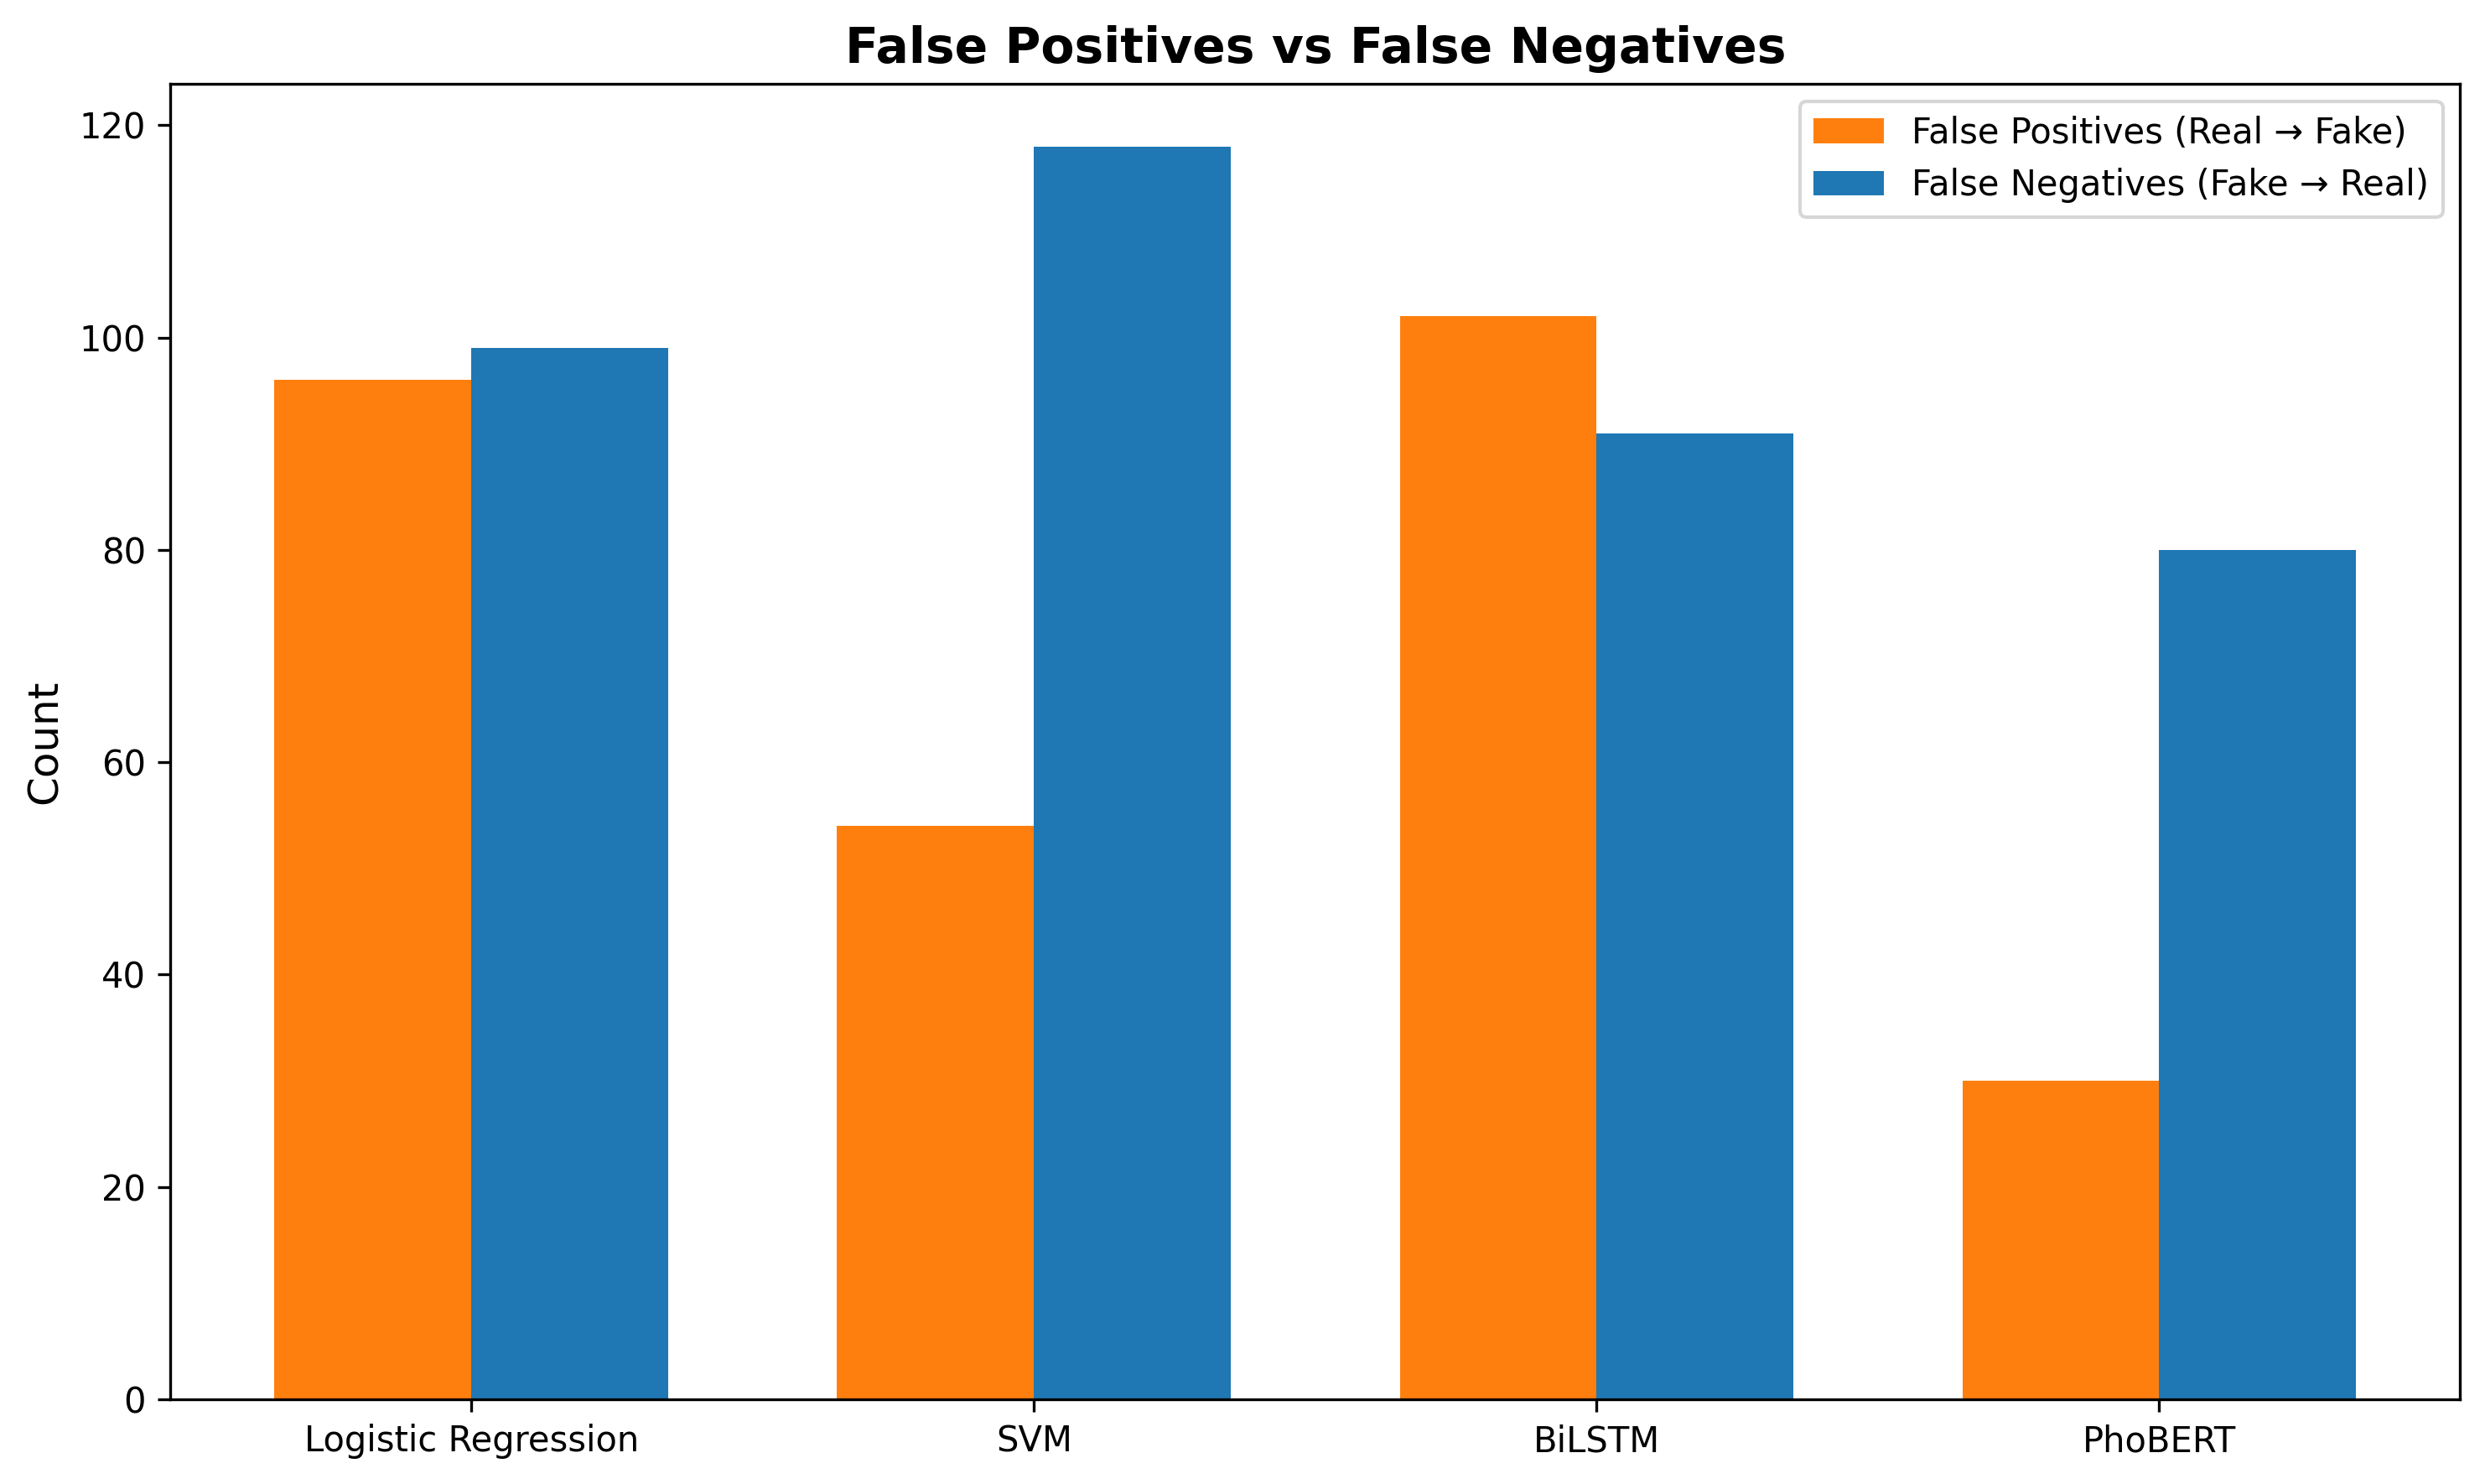
\includegraphics[width=0.6\textwidth]{fig_fp_fn_comparison}
\caption{So sánh số lượng False Positive (FP) và False Negative (FN) trong quá trình phân loại}
\label{fig:fpfn}
\end{figure}

Trong Hình~\ref{fig:fpfn}, số lượng \textit{false positive} (FP) và \textit{false negative} (FN) của từng mô hình được so sánh nhằm làm rõ các kiểu lỗi phổ biến trong bài toán phát hiện tin giả. Có thể quan sát rằng các mô hình khác nhau thể hiện xu hướng lỗi khác nhau. Logistic Regression tạo ra số lượng FP và FN khá cân bằng, trong khi SVM có xu hướng tạo ra nhiều FN hơn FP. Điều này cho thấy SVM thường bỏ sót một số trường hợp tin giả, đặc biệt khi các mẫu này không chứa các từ khóa đặc trưng rõ ràng.

Đối với BiLSTM, số lượng lỗi tổng thể cao hơn so với các mô hình còn lại, với cả FP và FN đều ở mức tương đối lớn. Điều này cho thấy mô hình tuần tự này chưa khai thác được đầy đủ thông tin ngữ nghĩa trong văn bản, có thể do kích thước dữ liệu huấn luyện chưa đủ lớn để học các biểu diễn ngữ cảnh phức tạp. Ngược lại, PhoBERT đạt số lượng lỗi thấp nhất trong bốn mô hình, phản ánh khả năng khai thác ngữ cảnh tốt hơn nhờ được tiền huấn luyện trên lượng lớn dữ liệu tiếng Việt.

Phân tích FP và FN cũng cho thấy một số đặc điểm của bài toán. Các FP thường xuất hiện ở những bài viết có tiêu đề mang tính giật gân hoặc chứa các từ khóa thường xuất hiện trong tin giả, khiến mô hình nhầm lẫn và dự đoán sai. Trong khi đó, các FN chủ yếu xảy ra ở những tin giả được viết theo phong cách trung lập hoặc có cấu trúc tương tự các bài báo chính thống, khiến mô hình khó phân biệt.

\subsubsection{Phân phối lỗi theo độ dài văn bản}

\begin{figure}[H]
\centering
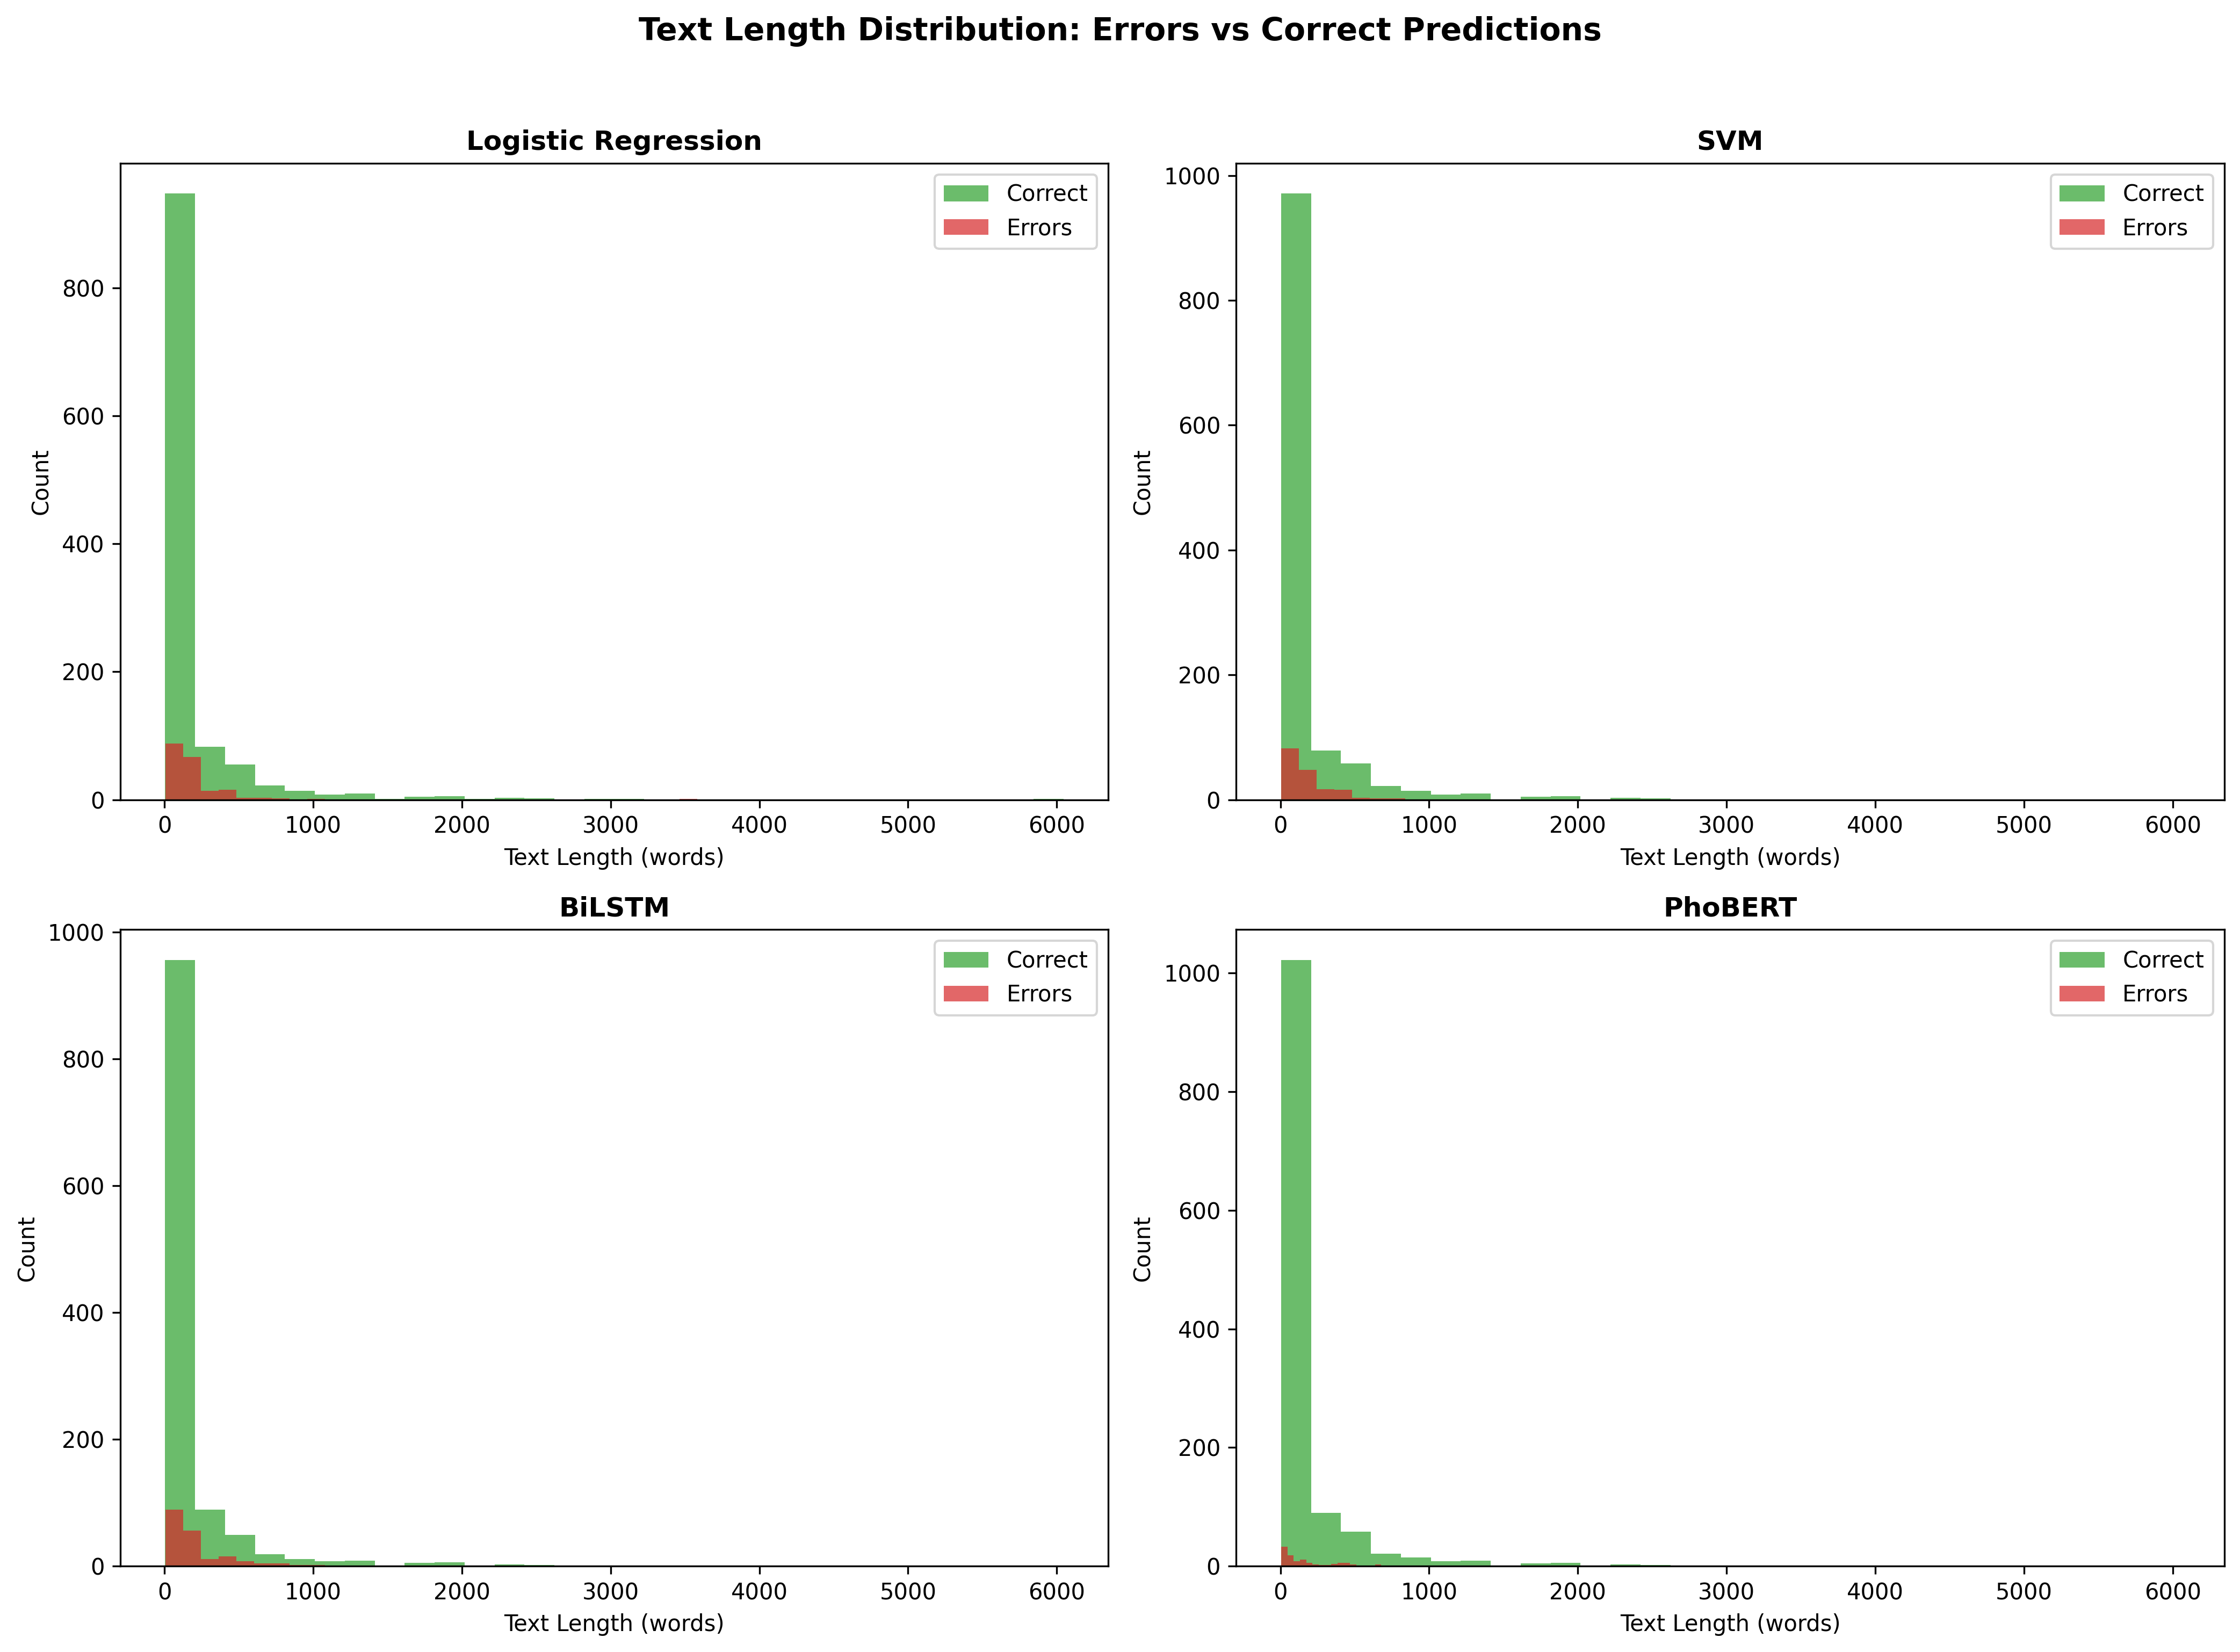
\includegraphics[width=0.9\textwidth]{fig_text_length_analysis}
\caption{Phân phối lỗi phân loại theo độ dài văn bản}
\label{fig:textlen}
\end{figure}

Hình~\ref{fig:textlen} minh họa phân phối các lỗi dự đoán theo độ dài văn bản đối với từng mô hình. Có thể thấy rằng phần lớn các lỗi xảy ra ở các văn bản có độ dài tương đối ngắn. Những văn bản ngắn thường thiếu ngữ cảnh và thông tin bổ sung cần thiết để mô hình có thể xác định chính xác tính xác thực của nội dung. Do đó, cả các mô hình học máy truyền thống và mô hình học sâu đều gặp khó khăn khi xử lý các mẫu này.

Ngược lại, khi độ dài văn bản tăng lên, tỷ lệ lỗi có xu hướng giảm. Các văn bản dài thường chứa nhiều thông tin ngữ nghĩa hơn, giúp mô hình nhận diện các mẫu đặc trưng liên quan đến tin thật hoặc tin giả một cách rõ ràng hơn. Xu hướng này đặc biệt rõ rệt đối với PhoBERT, khi mô hình tận dụng tốt hơn thông tin ngữ cảnh dài nhờ kiến trúc Transformer.

Phân tích này cho thấy độ dài văn bản là một yếu tố ảnh hưởng đáng kể đến hiệu năng của mô hình. Trong các ứng dụng thực tế, các bài viết ngắn hoặc tiêu đề đơn lẻ có thể cần được xử lý bằng các kỹ thuật bổ sung, chẳng hạn như kết hợp thông tin ngữ cảnh từ nguồn dữ liệu khác hoặc sử dụng các đặc trưng bổ sung ngoài nội dung văn bản.

\subsubsection{Hàm ý cải tiến mô hình}

\begin{table}[H]
\centering
\caption{Phân tích lỗi trên tập kiểm tra}
\label{tab:errors}
\begin{tabular}{lcccc}
\toprule
\textbf{Mô hình} & \textbf{Tổng lỗi} & \textbf{Tỉ lệ lỗi} & \textbf{FP} & \textbf{FN} \\
\midrule
Logistic Regression & \lrErrors & \lrErrorRate\% & \lrFPcount & \lrFNcount \\
SVM & \svmErrors & \svmErrorRate\% & \svmFPcount & \svmFNcount \\
BiLSTM & \bilstmErrors & \bilstmErrorRate\% & \bilstmFPcount & \bilstmFNcount \\
PhoBERT & \phobertErrors & \phobertErrorRate\% & \phobertFP & \phobertFN \\
\bottomrule
\end{tabular}
\end{table}

Bảng~\ref{tab:errors} tổng hợp số lượng lỗi và phân bố FP/FN của từng mô hình trên tập kiểm tra.

Từ các kết quả phân tích lỗi trên, có thể rút ra một số hướng cải tiến tiềm năng cho hệ thống phát hiện tin giả. Thứ nhất, việc kết hợp các đặc trưng ngữ nghĩa sâu với các đặc trưng bề mặt như từ khóa hoặc cụm từ đặc trưng có thể giúp giảm các trường hợp \textit{false positive} trong các mô hình học máy truyền thống. Thứ hai, các mô hình học sâu có thể được cải thiện bằng cách bổ sung thêm dữ liệu huấn luyện hoặc áp dụng các chiến lược tăng cường dữ liệu nhằm giúp mô hình học tốt hơn các mẫu tin giả được viết theo phong cách trung lập.

Ngoài ra, phân tích cũng cho thấy các văn bản ngắn là một nguồn gây lỗi phổ biến. Điều này gợi ý rằng các phương pháp khai thác ngữ cảnh mở rộng, chẳng hạn như kết hợp tiêu đề với nội dung bài viết hoặc tích hợp thông tin từ nguồn bên ngoài, có thể giúp cải thiện khả năng dự đoán đối với các trường hợp khó.

\subsubsection{Phân tích các trường hợp khó (Hard Examples)}

Mặc dù các phân tích trên đã chỉ ra một số nguyên nhân phổ biến gây ra lỗi phân loại, kết quả thực nghiệm cho thấy vẫn tồn tại một nhóm trường hợp đặc biệt khó mà tất cả các mô hình đều thất bại. Những trường hợp này phản ánh các giới hạn hiện tại của các phương pháp chỉ dựa trên nội dung văn bản và cung cấp thêm góc nhìn sâu hơn về những thách thức của bài toán phát hiện tin giả.

Trong quá trình phân tích lỗi, nhóm phát hiện \textbf{\nHardExamples{} mẫu khó} (\textit{hard examples}) mà tất cả bốn mô hình đều dự đoán sai. Việc kiểm tra thủ công nội dung của các mẫu này cho thấy chúng thường thuộc một số dạng đặc trưng, phản ánh những thách thức phổ biến trong bài toán phát hiện tin giả. Cụ thể, các trường hợp này có thể được chia thành ba nhóm chính: \textit{semantic reasoning}, \textit{knowledge verification}, và \textit{dataset ambiguity}.

Trước hết, một số mẫu yêu cầu suy luận ngữ nghĩa (\textit{semantic reasoning}) để xác định mối quan hệ giữa hai câu. Trong các trường hợp này, hai văn bản có thể không liên quan về mặt nội dung nhưng lại có phong cách viết tương tự, khiến mô hình khó phân biệt. Ví dụ, trong một mẫu dữ liệu, câu ``Uống đủ nước mỗi ngày hỗ trợ quá trình trao đổi chất của cơ thể.'' được ghép với câu ``Tỷ phú Phạm Nhật Vượng đã quyết định tặng 1000 xe VinFast VF9 cho các y bác sĩ chống dịch Covid-19.'' Hai câu này không có quan hệ ngữ nghĩa trực tiếp nhưng đều mang phong cách thông tin trung lập giống các bản tin, dẫn đến việc mô hình nhầm lẫn khi phân loại.

Thứ hai, một số trường hợp thuộc nhóm \textit{knowledge verification}, trong đó việc xác định tính đúng sai của thông tin đòi hỏi kiến thức thực tế ngoài văn bản. Ví dụ, câu ``Máy tính cá nhân đầu tiên được bán ra thị trường vào thế kỷ 18.'' là một khẳng định sai về mặt lịch sử công nghệ. Tuy nhiên, nếu chỉ dựa vào đặc trưng ngôn ngữ trong văn bản, mô hình khó có thể nhận biết được tính sai lệch của thông tin này. Điều này cho thấy các mô hình hiện tại chủ yếu học các mẫu ngôn ngữ bề mặt và chưa thể thực hiện kiểm chứng tri thức.

Cuối cùng, một số lỗi xuất phát từ \textit{dataset ambiguity}, tức là những trường hợp mà nội dung văn bản không cung cấp đủ ngữ cảnh để xác định nhãn một cách rõ ràng. Chẳng hạn, câu ``Hà Nội: học sinh từ cấp 2 trở lên dự kiến đi học trở lại từ 4/5.'' có hình thức giống một bản tin chính thống và không chứa dấu hiệu rõ ràng của thông tin sai lệch. Trong các trường hợp như vậy, việc phân loại có thể phụ thuộc vào bối cảnh thời gian hoặc nguồn tin, điều mà các mô hình chỉ dựa trên văn bản không thể khai thác.

Những quan sát này cho thấy các lỗi còn lại không chỉ xuất phát từ hạn chế của mô hình mà còn phản ánh độ phức tạp của bài toán phát hiện tin giả. Các hệ thống trong tương lai có thể được cải thiện bằng cách tích hợp thêm nguồn tri thức bên ngoài hoặc các cơ chế suy luận ngữ nghĩa sâu hơn.
\subsection{Phân tích khả năng giải thích}

\begin{figure}[H]
  \centering
  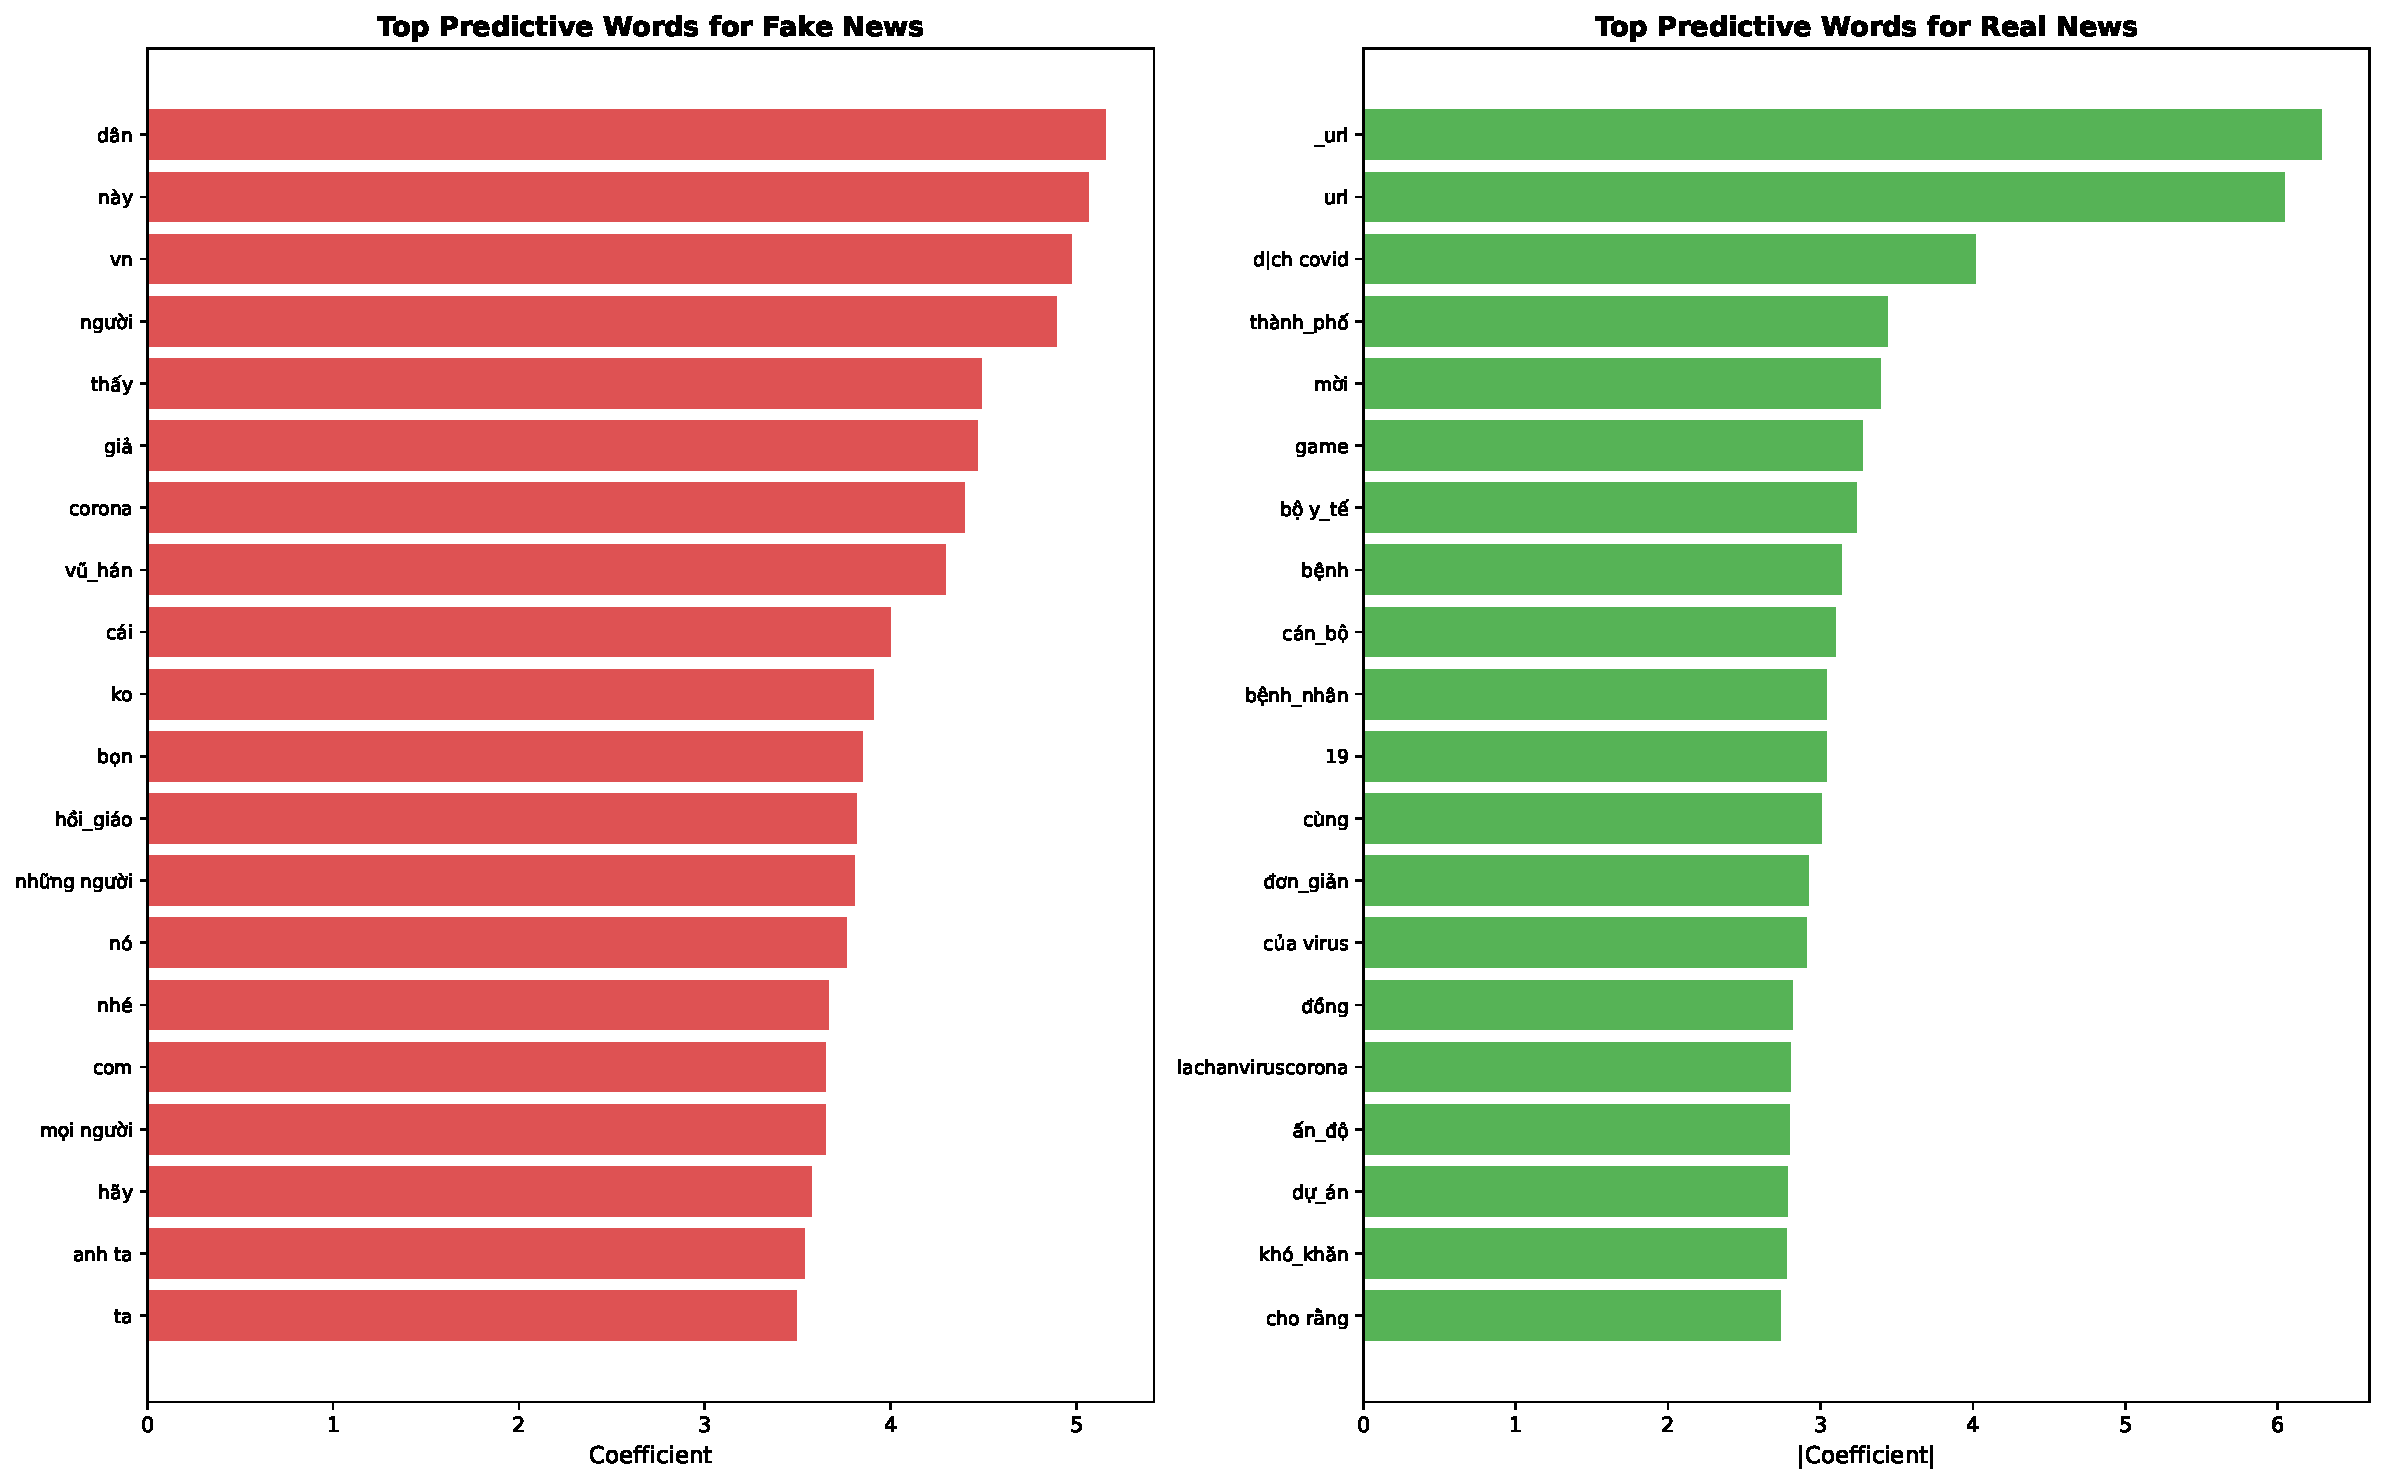
\includegraphics[width=0.95\textwidth]{feature_importance}
  \caption{Top 15 đặc trưng TF-IDF có hệ số LR cao nhất (dương = chỉ điểm Giả, âm = chỉ điểm Thật)}
  \label{fig:feature_importance}
\end{figure}

Hình~\ref{fig:feature_importance} minh họa 15 đặc trưng TF-IDF có hệ số lớn nhất trong mô hình Logistic Regression. 
Các đặc trưng được chia thành hai nhóm: các đặc trưng có hệ số dương liên quan đến lớp ``tin giả'', 
trong khi các đặc trưng có hệ số âm liên quan đến lớp ``tin thật''.

Có thể quan sát rằng nhiều từ khóa liên quan đến tin giả thường mang tính giật gân hoặc gây chú ý, 
ví dụ các cụm từ mang sắc thái khẳng định mạnh hoặc gây tò mò. 
Ngược lại, các từ khóa liên quan đến tin thật thường xuất hiện trong văn phong báo chí chính thống, 
chẳng hạn như các từ liên quan đến cơ quan nhà nước, tổ chức hoặc thuật ngữ chính sách.

Kết quả này cho thấy mô hình Logistic Regression không chỉ học các đặc trưng tần suất đơn thuần 
mà còn khai thác được những mẫu ngôn ngữ đặc trưng của từng loại tin. 
Điều này giúp tăng tính minh bạch của mô hình, 
vì các quyết định phân loại có thể được giải thích trực tiếp thông qua các trọng số đặc trưng.

\begin{figure}[H]
  \centering
  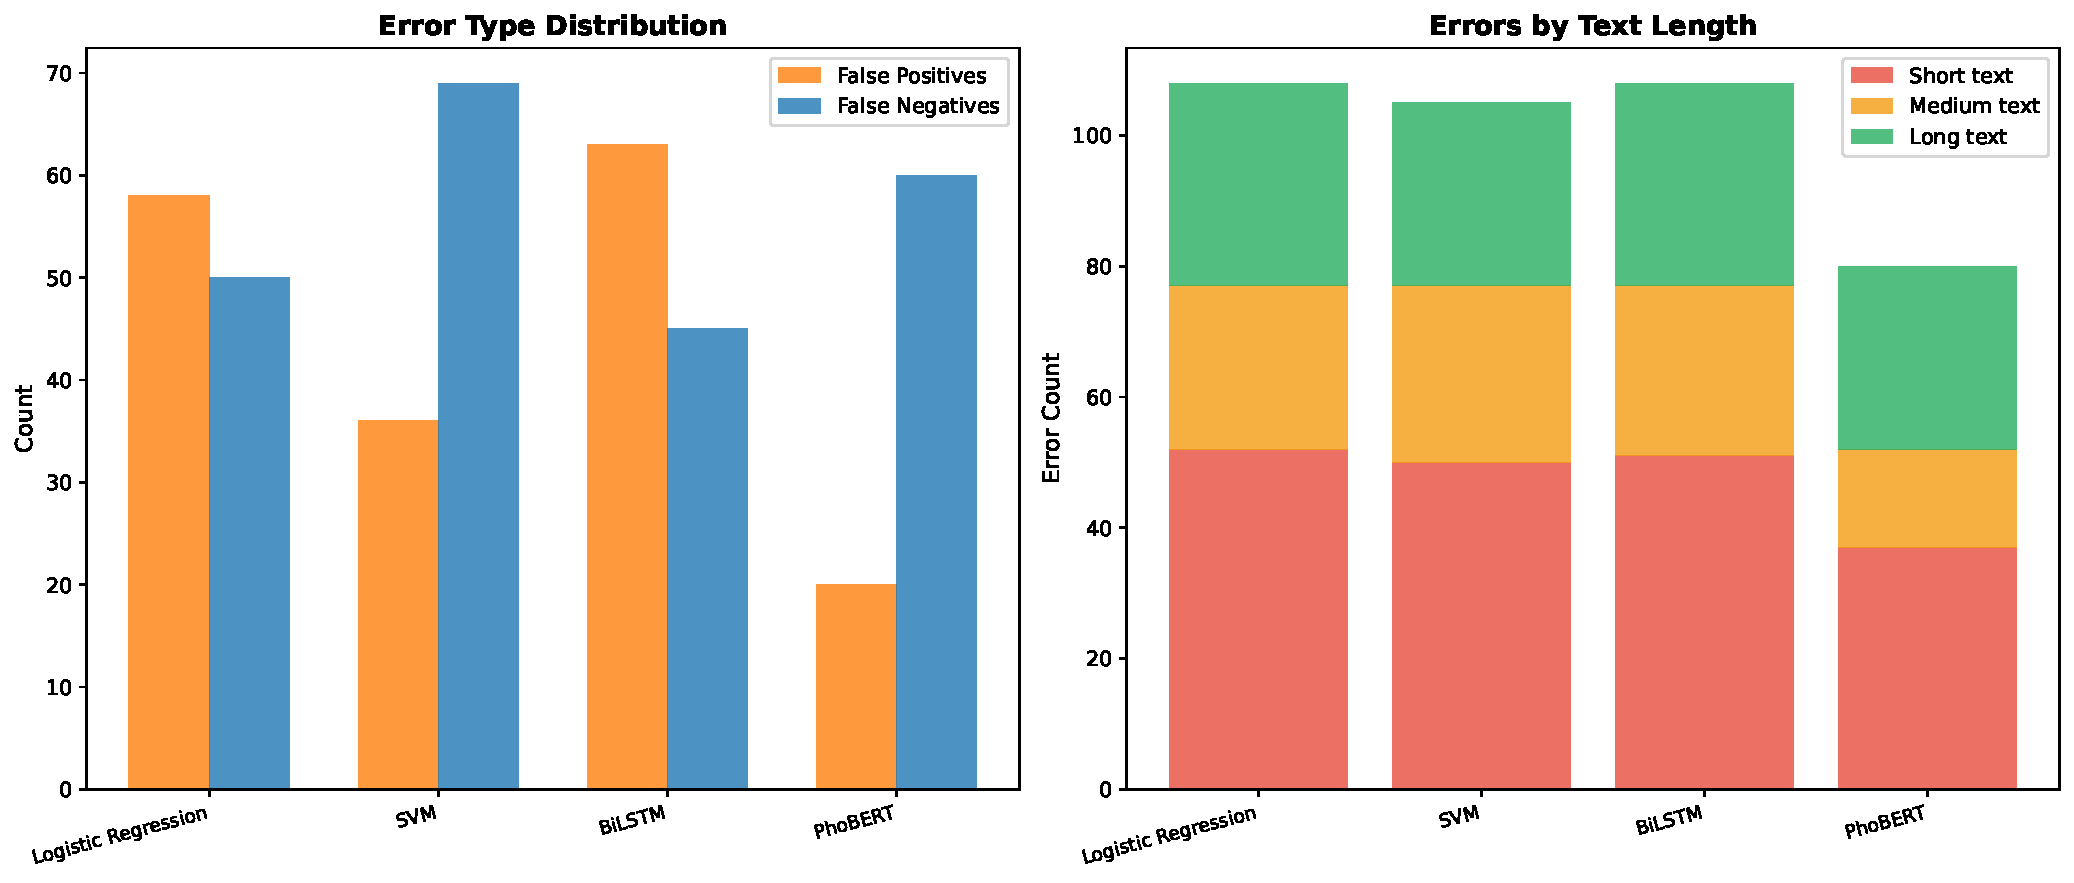
\includegraphics[width=0.85\textwidth]{error_taxonomy}
  \caption{Phân loại lỗi theo độ dài văn bản và mức độ tin cậy dự đoán}
  \label{fig:error_taxonomy}
\end{figure}

Hình~\ref{fig:error_taxonomy} trình bày phân tích lỗi theo độ dài văn bản 
và mức độ tin cậy của dự đoán.

Ở biểu đồ bên trái, có thể quan sát rằng số lượng lỗi cao hơn đối với các văn bản ngắn. Điều này có thể được giải thích bởi việc các văn bản ngắn thường thiếu ngữ cảnh 
và chứa ít đặc trưng TF-IDF hơn, khiến mô hình khó phân biệt giữa tin thật và tin giả.

Biểu đồ bên phải cho thấy phần lớn các lỗi xảy ra ở các dự đoán có mức độ tin cậy thấp hoặc trung bình. 
Trong khi đó, các dự đoán có độ tin cậy cao hiếm khi bị sai. 
Kết quả này cho thấy xác suất dự đoán của mô hình có tương quan tốt với độ chính xác thực tế.

Phân tích này gợi ý rằng trong các ứng dụng thực tế, 
những dự đoán có độ tin cậy thấp có thể được chuyển sang bước kiểm tra thủ công 
hoặc kết hợp với các hệ thống fact-checking để tăng độ tin cậy tổng thể của hệ thống.

\section{Kết luận chương}

Thực nghiệm toàn diện xác nhận \phobert là mô hình tốt nhất (F1 = \phobertFone\%) và vượt trội có ý nghĩa thống kê. Tiền huấn luyện trên ngữ liệu tiếng Việt là yếu tố quyết định, không phải kiến trúc phức tạp. SVM vượt BiLSTM là minh chứng rõ ràng cho vai trò của đặc trưng chất lượng trong học máy truyền thống.

% ============================================================
%  KẾT LUẬN
% ============================================================
\chapter*{Kết luận}
\addcontentsline{toc}{chapter}{Kết luận}

\section*{Tóm tắt đóng góp}

Nghiên cứu xây dựng và so sánh bốn phương pháp phát hiện tin giả tiếng Việt trên bộ dữ liệu \nClean{} mẫu. Kết quả chính:

\begin{itemize}[leftmargin=2em]
  \item \textbf{PhoBERT} đạt hiệu năng tốt nhất: Accuracy = \phobertAcc\%, F1 = \phobertFone\%, AUC = \phobertAUC.
  \item Cải thiện \textbf{+\deltaLR\%} F1 so với baseline Logistic Regression.
  \item Kiểm định McNemar xác nhận sự vượt trội \textbf{có ý nghĩa thống kê} ($p < 0.001$).
  \item SVM vượt BiLSTM, minh chứng cho tầm quan trọng của chất lượng đặc trưng hơn độ phức tạp kiến trúc.
  \item Tiền huấn luyện trên tiếng Việt là nhân tố quyết định; phân đoạn từ ảnh hưởng ít với TF-IDF nhưng quan trọng với PhoBERT.
  \item Phân tích lỗi xác định \nHardExamples{} mẫu khó và cho thấy tin giả hay giả mạo phong cách thông tấn quốc tế.
\end{itemize}

\section*{Hạn chế}

\begin{itemize}[leftmargin=2em]
  \item Tập dữ liệu có thể chưa bao phủ đầy đủ tất cả các thể loại và chiến thuật lan truyền tin giả trong thực tế, đặc biệt là các nội dung mới xuất hiện hoặc có tính chuyên biệt theo từng miền.
  
  \item Mô hình có thể suy giảm hiệu năng khi áp dụng trên dữ liệu ngoài miền huấn luyện (domain shift), đặc biệt đối với các hình thức ngụy trang tinh vi hoặc biến thể ngôn ngữ mới.
  
  \item Mô hình PhoBERT yêu cầu tài nguyên tính toán tương đối lớn, điều này có thể gây hạn chế khi triển khai trong môi trường thực tế quy mô lớn hoặc thời gian thực.
\end{itemize}
\section*{Hướng phát triển}

\begin{itemize}[leftmargin=2em]
  \item Thu thập thêm dữ liệu đa dạng thể loại tin giả tiếng Việt.
  \item Tích hợp thông tin đa phương thức (hình ảnh, đồ thị lan truyền mạng xã hội).
  \item Xây dựng hệ thống phát hiện thời gian thực với PhoBERT được nén nhỏ (knowledge distillation)~\cite{hinton2015distilling}.
  \item Kết hợp kiểm chứng thực tế (fact-checking) với phân loại tự động.
\end{itemize}

% ============================================================
%  TÀI LIỆU THAM KHẢO
% ============================================================
\bibliographystyle{IEEEtran}
\bibliography{references}

\end{document}
